\chapter{基于多方联邦的半监督学习方法} % 定义章节,章节标题为“图表、公式格式和印制要求Abc”

\thispagestyle{others} % 设置当前页面的页眉页脚样式为“others”,该样式需要用户自行定义

\pagestyle{others} % 设置后续页面的页眉页脚样式为“others”,该样式同样需要用户自行定义

\xiaosi % 可能是自定义的命令,通常用于调整字体大小或格式,需要在前文定义


\section{本章引言}
联邦学习(Federated Learning, FL)作为一种新兴的分布式机器学习方法,为多方协作数据隐私保护问题提供了一种解决方案\textsuperscript{\cite{mcmahan2017communication}}。联邦学习允许多个数据所有者(客户端)在不共享原始数据的前提下,通过交换模型参数或梯度实现联合训练。现有联邦学习方法主要集中在监督学习场景,但在现实中,由于标注成本高、领域专家稀缺或资源受限等原因,数据往往并不完全标记。因此,近年来研究者开始探索半监督学习(Semi-Supervised Learning, SSL)在联邦学习场景下的应用,特别是仅包含正样本和未标记数据的PU(Positive and Unlabeled)学习问题。目前已有一些代表性方法被提出,如:FedPU算法\textsuperscript{\cite{lin2022federated}}通过PU学习策略提高有限标记数据的联邦学习性能;RSCFed算法\textsuperscript{\cite{liang2022rscfed}}通过聚合多个子共识模型以处理本地客户端的非独立同分布(Non-IID)问题;FedMatch算法\textsuperscript{\cite{jeong2020federated}}优化客户端间参数一致性与分解策略,改善有限标记数据下的联邦学习效果;AdaFedSemi算法\textsuperscript{\cite{wang2022enhancing}}则借助多臂赌博机优化客户端参与度与伪标签质量,提升半监督联邦学习的性能。

上述场景属于HFL,即多个数据所有者共享相同的特征空间,但样本ID空间不同。尽管VFL在隐私保护机器学习领域具有重要的应用价值,但当前针对VFL场景下的半监督学习研究仍然较为稀少,尤其是在PU学习问题上的探索几乎处于空白状态。

在纵向联邦学习的实际应用中,往往存在这样一种特殊的PU学习问题:数据分布方面,不同的数据所有者(机构)拥有部分重叠的样本ID,但特征空间不重合且各方数据具有专有性;数据类型方面,通常目标方仅持有标记为正类的数据,其他参与方则仅持有未标记数据,并且所有方之间无法直接访问对方的原始数据;在这种情形下,各方希望联合训练一个有效的机器学习模型,用于从未标记数据中精准识别出可靠的正样本,同时保证各自数据的隐私安全。

此类特殊的PU学习场景在多个重要行业领域有着广泛的实际应用背景。在医疗健康领域,某医疗机构(目标方)拥有确诊患有特定疾病的患者记录(正样本),包含患者ID及其诊断结果;而合作的医学检验机构、影像中心等(参与方)拥有更多患者的各类检测数据,但缺乏确诊标签。在保护患者隐私的前提下,各方希望通过联合建模来从未确诊人群中识别潜在的高风险患者。类似地,在金融风控领域,银行(目标方)掌握已确认的欺诈交易记录(正样本),而支付平台、电商平台等合作方(参与方)拥有大量未标记的交易行为数据。由于数据合规要求,各方无法直接共享数据,但希望协作构建模型以识别可疑交易。这些现实场景清晰地展示了一个共同特点:目标方仅掌握正类样本,而参与方则持有大量未标记数据,但各方出于隐私保护和数据合规的考虑无法直接共享原始数据。这种数据分布模式恰好对应了PU学习问题的典型特征,即需要仅凭正样本和未标记数据来构建有效的分类模型。

这些场景中,目标方只拥有正样本,而其他方仅拥有未标记数据,恰好对应了PU学习问题的典型特征,即仅凭正样本和未标记数据来构建有效的分类模型。然而,现有的PU学习方法\textsuperscript{\cite{mordelet2014bagging, liu2003building, liu2015classification, xu2017multi}} 一般都默认正样本和未标记数据在训练过程中可以同时访问,而在VFL场景下,由于数据分布于不同的机构之间并且无法直接共享,这种传统PU学习框架无法直接适用于该场景。这导致了一个全新的挑战,即未标记数据缺失的PU学习问题(Unlabeled-Data-Deficient PU, UDD-PU)。

为应对这一挑战,本章提出了基于正样本和未标记数据的纵向联邦学习方法(Vertical Federated Learning with Positive and Unlabeled data, VFPU)。VFPU允许多个数据所有者在不暴露自身原始数据的前提下,通过协作训练一个联合模型,实现在未标记数据中有效识别正样本。VFPU方法在保障数据隐私的基础上,仅通过交换加密后的中间计算结果完成联邦训练过程;同时,该方法融合了PU学习策略,能够在纵向联邦学习场景下充分利用未标记数据,提升模型的分类性能。此外,VFPU具备广泛的应用前景,能够有效应对金融、医疗、智能制造等多个领域的数据孤岛问题,满足实际应用中日益严格的数据隐私保护要求。

本章后续的结构安排为:3.2节对问题进行分析与定义。3.3节介绍方法的核心内容,包括数据预处理与加密样本对齐,以及VFPU算法的执行。3.4节详细说明实验设计、数据集准备及实验结果分析。最后,3.5节对本章内容进行总结。


\section{问题分析与定义}
在本章节讨论的语境中,首先探讨一个分布式数据场景:K个独立的数据所有者各自掌控着大型数据集的不同部分,并存在一个中央服务器作为协作协调者。每个数据所有者持有的数据被系统地组织成矩阵形式,具体记作${{\mathsf{\mathcal{D}}}_{k}}$(下标k表示第k个数据所有者)。该矩阵中,每行对应一个独立样本(即具体的数据实例或观测值),每列对应特定特征(即样本的可测量属性或特性)。从全局视角,整个分布式数据集可抽象为结构化三元组$(\mathsf{\mathcal{I}}, \mathsf{\mathcal{X}}, \mathsf{\mathcal{Y}})$,其中:$\mathsf{\mathcal{I}}$为样本ID空间,包含所有样本的唯一标识符;$\mathsf{\mathcal{X}}$为特征空间,涵盖所有样本的全部特征维度;$\mathsf{\mathcal{Y}}$为标签空间:包含所有可能的分类标签或类别。

在传统纵向联邦学习(Vertical Federated Learning, VFL)框架中,通常存在一个关键假设:至少有一个参与方持有其数据部分的完整标签集,从而能够实现有监督的预测模型训练。然而,这一假设在大量现实场景中往往难以成立,因为获取全量标注数据集面临严峻挑战。这种挑战主要源于实际商业环境中的多重约束,包括但不限于:隐私保护法规对数据使用的限制、高昂的人工标注成本、行业竞争导致的数据孤岛现象、敏感信息共享的法律风险以及动态数据更新带来的标注滞后问题。

为了更清晰、更具体地理解这一问题,现在考虑一个具体的示例场景,其中涉及三位不同的数据拥有者,将其分别称为 A 方、B 方和 C 方。这三方各自持有敏感数据——这些信息对其业务至关重要,但由于隐私和安全方面的考虑,他们不愿直接公开。因此,他们需要在确保数据隐私严格保护的前提下,以安全的方式进行合作,充分利用各自的数据资源。

在该场景中,所涉及的数据样本可以被划分为两大基本类别:正类(positive)和负类(negative),这可以对应于某些应用场景中的理想(或期望)行为与非理想(或不期望)行为。一个值得注意的特点是,这三方在样本标识符(ID)上存在一定程度的重叠,即某些样本可能同时出现在多个参与方的数据集中,但每一方所收集或观察到的特征可能有所不同。

具体而言,A 方持有一个样本集合,记作 $ P $,该集合的独特之处在于它仅包含正类样本——即被明确标记为正类的数据实例,不包含任何负类或不确定的样本。而 B 方和 C 方共同持有一个未标注数据集,记作 $ U $,其中的样本类别(正类或负类)未知。需要特别强调的是,$ U $ 不包含 A 方数据集 $ P $ 中的任何样本,即 $ U $ 是一个独立的数据集,不与 A 方的正类样本重叠。

这三方的主要目标是通过合作共同训练一个推荐模型,该模型的作用是分析未标注数据集 $ U $,并从中识别出可以被可靠归类为正类的样本。这一过程的输出结果记作 $ R $,即从 $ U $ 中成功提取出的可靠正类样本集合。一旦这些样本被识别出来,$ R $ 将被提供给 A 方,使其能够基于这些推断出的正类实例向客户或用户提供精准的产品推荐,从而提升其业务能力和市场竞争力。

该问题设置引入了一个挑战,使得传统的纵向联邦学习(VFL)算法在其标准形式下无法适用。核心问题在于,参与的各方——A 方、B 方和 C 方——都不拥有完整的标签数据。在传统的 VFL 方案中,至少需要有一方持有完整的标注数据,以便模型能够从监督信号中学习,并在联邦系统中传播。然而,在本问题中,A 方仅拥有正类样本的标签(即数据集 $ P $),而 B 方和 C 方的数据集 $ U $ 完全没有标签,这导致了一个关键的缺口,使得标准的 VFL 技术无法直接应用。

为了应对这一挑战,可以考虑采用半监督学习(semi-supervised learning)策略,该策略专门用于处理包含部分标注数据和未标注数据的场景。在本问题背景下,一个特别相关的方法是PU 学习(Positive and Unlabeled learning,正类与未标注学习)。PU 学习是一种特殊的半监督学习技术,它利用一组带有正类标签的样本($ P $)和一组未标注样本($ U $)进行训练,目标是在未标注数据集中识别出正类实例。PU 学习特别适用于缺少负类标签或负类标签不可靠的情况,因此在本问题中具有较大的应用潜力。

然而,PU 学习在本场景下的直接应用存在一个关键限制:传统的 PU 学习方法假设学习者可以同时访问 $ P $ 和 $ U $,从而能够直接对比正类样本和未标注样本,并进行有效的训练。然而,在本联邦学习场景中,这一假设并不成立,因为 A 方仅持有 $ P $,而 $ U $ 分布在 B 方和 C 方手中。由于隐私保护的要求,各方无法简单地将数据汇总到一个集中存储库,也不能自由共享数据给 A 方,这使得传统 PU 学习方法难以直接应用,成为本问题的一个重要挑战。

在这种情况下,A 方希望将推荐服务集成到其业务运营中,但面临一个全新的复杂挑战,将其称为“未标记数据缺失的 PU 学习问题”(Unlabeled-Data-Deficient PU, UDD-PU)。该问题的核心特征在于,A 方仅能访问正类样本集 $ P $,但无法直接获取未标注数据 $ U $,这使得传统的 PU 学习方法无法直接应用。此外,由于数据在联邦学习环境下分布——即 $ U $ 分散存储在 B 方和 C 方手中——并且所有参与方都施加了严格的隐私保护要求,现有的 PU 学习方法若不进行改进,无法直接适用于该场景。

UDD-PU 问题代表了联邦学习、半监督学习和隐私保护计算的独特交汇点,需要创新性的解决方案,以便在这些约束条件下实现有效的协作和模型训练。


\section{基于多方联邦的半监督学习方法}
在推荐系统中,有效利用多个参与方的数据,同时应对特定挑战至关重要。在某些场景下,会出现 UDD-PU 学习问题,即某一方(在本例中为 A 方)缺乏足够的未标记样本,导致无法使用传统的PU学习技术来有效训练推荐模型。这种未标记数据的不足会影响模型的泛化能力,导致性能下降和推荐结果不够准确。为了解决这一问题,本章提出了 VFPU 算法,这是一种结合了纵向联邦学习框架与 PU 学习技术的新方法。VFPU 旨在解决 A 方未标记样本不足的问题,通过更好地利用分布式数据资源,提升推荐模型的性能。

在本章中,基于 VFPU 的推荐过程主要包括三个核心步骤:数据预处理、加密样本对齐以及 VFPU 算法的执行。这些步骤共同构成了一个稳健的流程,以在隐私保护的协作环境中提升推荐的准确性。VFPU 的主要目标是在多个参与方持有的未标记数据集中识别可靠的正例样本。通过精准定位这些可靠的正例样本,模型能够更好地区分正例和负例,即便在缺乏明确标注的负例数据的情况下——这是 PU 学习场景中的常见挑战。

这一能力在推荐系统中尤为关键,因为用户偏好通常是通过交互隐式表达的,而非通过显式标签标注。因此,模型需要从有限或噪声较大的数据中推断用户偏好。通过识别这些可靠的正例样本,模型能够更深入地理解正向实例的特征,例如用户偏好或产品相关性,从而最终生成更准确、更个性化的产品推荐,以满足 A 方的需求。

对于 A 方而言,由于数据资源有限,其推荐模型的性能可能受到约束。然而,通过这一联邦学习方法,A 方可以利用 B 方和 C 方的丰富数据集,从而显著增强推荐模型的稳健性。同时,确保数据隐私的保护,并促进多个参与方之间的无缝协作,严格遵循联邦学习的核心原则。在整个过程中,数据隐私得到了精心维护,每个参与方的原始数据始终保持本地化,仅共享模型更新或聚合后的信息,而不会泄露敏感的个人记录。

这种隐私保护的协作方式在 图 \ref{fig:VFPU} 中得到了展示,该图详细说明了推荐过程的具体流程。本章的后续章节将对这一过程中的各个步骤进行深入探讨,以提供对该方法的全面理解。

\vspace{-0.1cm}
\begin{figure}[h]
	\centering
	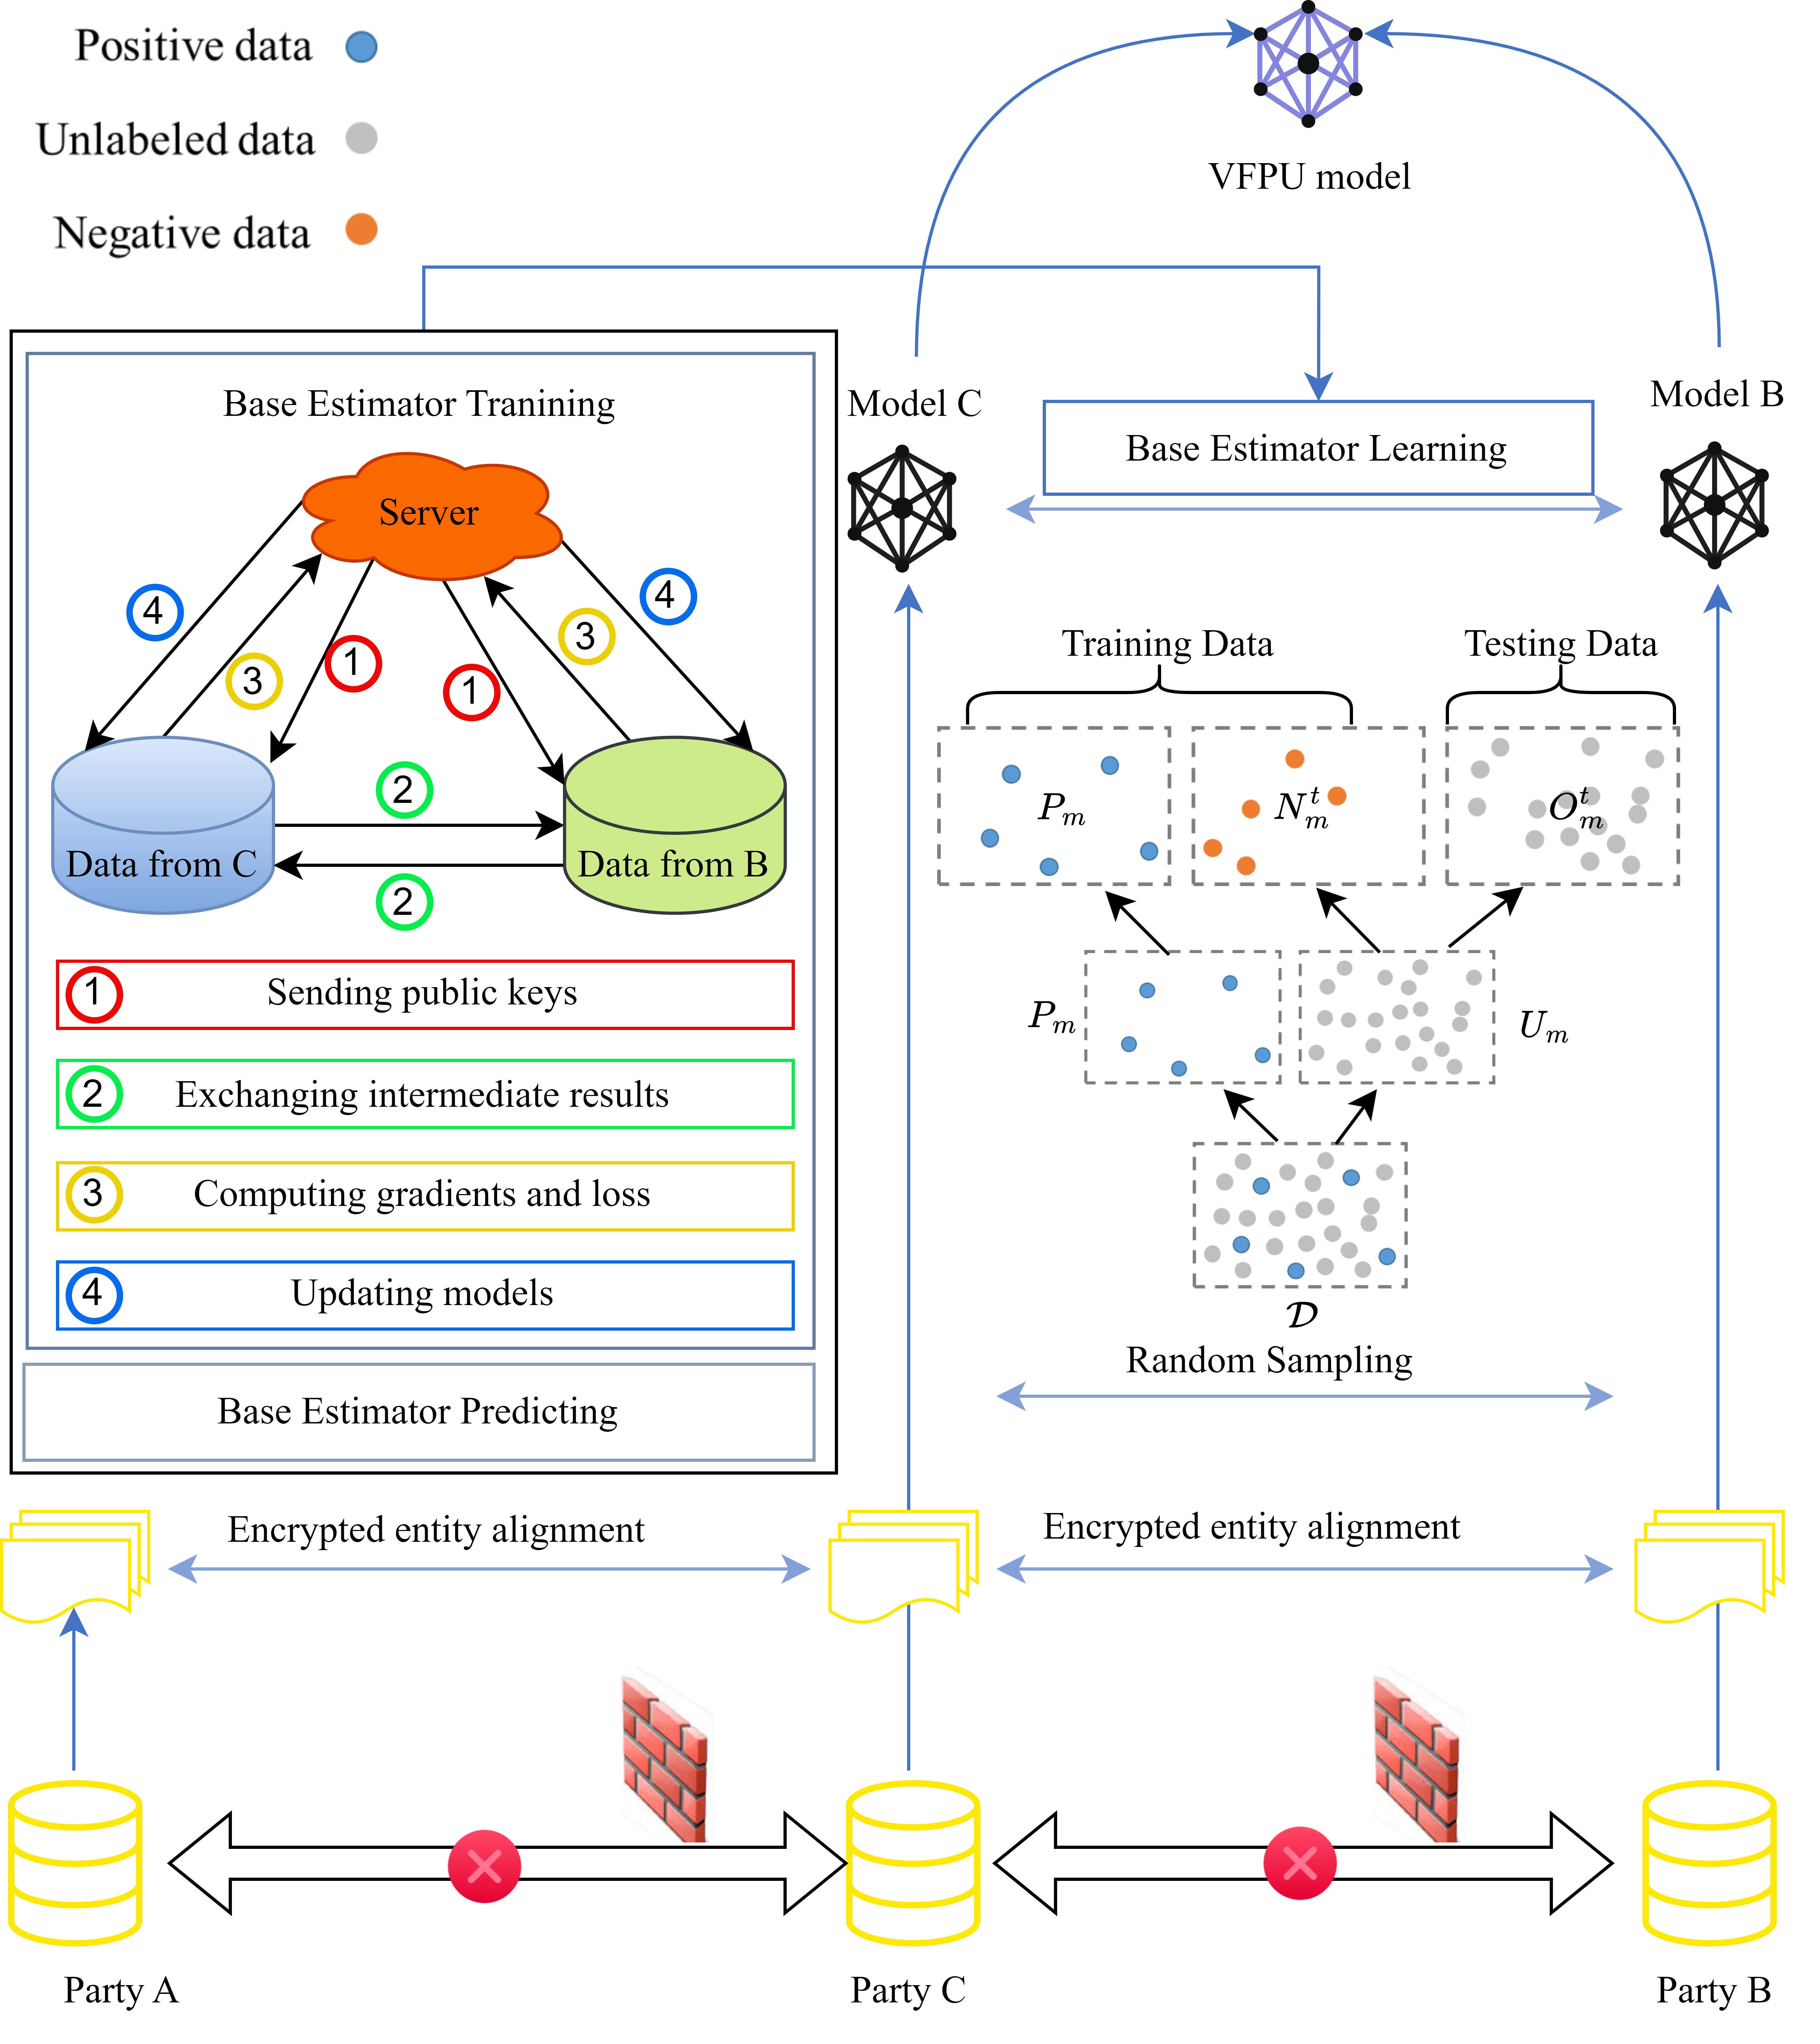
\includegraphics[width=0.9\textwidth]{chapters/imgs/Figure 1 in JEPG format}
	\bicaption[\xiaosi VFPU算法总体流程]
	{\wuhao VFPU算法总体流程}
	{\wuhao The overall process of the proposed VFPU algorithm}
	\label{fig:VFPU}
\end{figure}
\vspace{-0.35cm}

\subsection{数据预处理与加密样本对齐}
为了有效地训练模型,VFPU框架包含了一个两部分的预处理阶段:数据预处理和加密样本对齐。这些过程确保了来自A、B和C方的数据集在不损害隐私的情况下进行协调和安全对齐。 

(1) 数据预处理 

对A、B和C方持有的异构数据应用各种预处理技术,包括数据清洗、规范化和特征编码。数据清洗是第一步,它涉及解决常见的数据质量问题,例如通过插补或删除处理缺失值,消除重复项,并解决数据收集过程中可能出现的错误。这些努力确保数据集可靠,并且没有可能扭曲模型性能的噪声。规范化紧随其后,确保各方所有特征都达到可比的规模,这对许多机器学习算法的最佳运行至关重要。具体来说,数值特征使用标准化缩放进行规范化,这是一种将数据转换为零均值和单位方差的技术,从而防止范围较大的特征不成比例地影响模型。同时,分类特征通常表示定性属性,例如产品类别或用户人口统计信息,使用独热编码进行处理。此方法通过为每个类别创建二进制向量来将分类变量转换为数字格式。总之,这些预处理步骤创建了一个标准化、高质量的数据集,为后续处理做好准备。

(2) 加密样本对齐

在数据预处理之后,三方参与一个安全的样本对齐过程,该过程分两个不同的步骤进行,以同步其数据集,同时保护隐私。这种对齐对于实现纵向联邦学习至关重要,在纵向联邦学习中,各方持有重叠样本集的互补特征。 

步骤 1: B方和C方对齐其样本 ID 空间,仅保留两方共享的样本,丢弃未对齐的样本。此步骤确保B方和C方在一个共同的样本集上进行操作,这是纵向联邦学习的前提条件。在此过程中,通过关注样本集的交集,B方和C方的特征能够对应于相同的实体,从而建立一个一致的基础,使得模型可以有效地在组合特征空间中进行学习。因此,B方和C方在共享相同样本的基础上,保持各自独特且互补的特征,为协同训练奠定了基础。

步骤 2: A方和C方对齐其样本 ID 空间,不删除任何样本,与步骤 1 相比采用了一种更具包容性的方法。对齐的样本定义为存在于A方和C方数据集中的样本,而未对齐的样本仅存在于C方。这种对齐过程利用了来自A方的可用标签信息来丰富C方的数据集。具体来说,出现在A方和C方中的样本在C方中被分配一个标签 1,表示它们是正样本,因为它们对应于A方数据中已知的正实例。C方中缺少A方对应物的样本被分配一个标签 -1,将其标记为可能包含正负实例混合的未标记样本。这种标记策略将C方的数据集转换为适合 PU 学习的数据集,其中挑战在于区分未标记集中真正的正样本。通过不丢弃任何样本,此步骤最大限度地利用了可用于训练的数据,同时利用A方的正样本来指导该过程。

在完成加密样本对齐后,C方获得了一个包含正样本和无标签样本的数据集。这种转换有效地将原始的UDD-PU推荐问题——其特点是A方缺乏无标签数据——转变为一个纵向联邦训练场景。在这个场景中,PU学习问题由B方和C方协作解决,其中B方提供额外的特征,C方提供有标签和无标签的样本。这种合作框架充分利用了所有方的优势,克服了A方在数据方面的限制,最终使其推荐系统受益。

为了在样本对齐过程中保护数据隐私,采用了基于盲RSA的私有集交集(PSI)协议 \textsuperscript{\cite{de2010practical}}。这种密码学技术使所有方能够安全地计算其数据集的交集,而不会暴露除共享样本ID之外的任何信息。具体来说,PSI确保B方和C方能够识别它们的共同样本,同时A方和C方能够确定它们的重叠样本,而不会泄露各自数据集的全部内容或关于未对齐样本的任何敏感细节。这种保护隐私的机制是联邦学习范式的核心,促进了各方之间的信任,并确保遵守数据保护标准。随着数据预处理和加密样本对齐的顺利完成,B方和C方的数据集现已完全准备就绪——经过对齐、标记和保护——可以用于执行VFPU算法。基于此处奠定的基础,该算法及其训练过程的细节将在后续章节中详细阐述。


\subsection{基于正样本与未标记数据的纵向联邦学习}
VFPU算法的目标是在纵向划分的数据环境中,安全且高效地从未标记数据中识别可靠的正例样本。这种场景在现实应用中经常出现,其中不同的组织持有相同数据主体的不同特征,但由于隐私问题或法规限制,无法直接共享原始数据。例如,银行可能拥有金融交易记录,而电子商务平台则掌握在线购物历史,这些数据都与相同的客户相关。识别正例样本(如可能违约的贷款客户或可能响应特定营销活动的客户)至关重要,但由于缺乏完整的标注数据以及特征的分布式存储,这一任务极具挑战性。

VFPU 通过巧妙结合既有的PU学习技术和纵向联邦学习框架来应对这一挑战。具体而言,它利用了 Liu 等人\textsuperscript{\cite{liu2003building}} 提出的两步技术,以及 Mordelet 和 Vert \textsuperscript{\cite{mordelet2014bagging}} 提出的 PU bagging 方法的鲁棒性。这些方法经过调整和整合,形成了一种安全协议,使得各方能够在不泄露数据隐私的情况下进行协作训练。

算法 3-1 详细描述了 VFPU 过程。第一阶段采用两步技术,首先从未标记数据中识别出一组可靠的负例样本。这一过程利用了正例样本,并假设未标记数据中同时包含正例和负例。通过仔细分析特征分布,可以提取出可靠的负例集合,从而更准确地表示数据的真实分布。随后,利用这些可靠的负例样本以及原始的正例样本训练一个初步分类模型,以该模型作为第二阶段的基础。

第二阶段引入 PU bagging 方法,以进一步增强 VFPU 的鲁棒性和性能。通过从正例和可靠负例集合中生成多个自助采样(bootstrap)样本,并在每个样本上训练独立的分类器,PU bagging 有效地缓解了初始可靠负例选择可能带来的偏差。最终预测结果通过集成这些独立分类器的预测结果获得,从而在未标记数据中更稳定、准确地识别正例样本。这种集成方法还增强了 VFPU在处理噪声数据或不完整数据时的适应能力,而这些问题在现实数据集中普遍存在。此外,纵向联邦学习框架确保了整个过程中的数据隐私收到保护。每个参与方都保留对自身数据的控制权,并且在训练过程中仅共享中间结果(如模型参数或加密梯度)。这种去中心化的方法避免了集中式数据存储的需求,并最大程度地降低了数据泄露的风险。

\vspace{-0.1cm} 
\begin{table}[h]
	\renewcommand{\arraystretch}{0.6}
	\centering
	{\songti \wuhao
		\begin{tabular}{p{\textwidth}}
			\toprule[1.5pt]
			\makecell[l]{\songti\wuhao 算法3-1 VFPU 算法训练过程}\\
			\midrule[0.75pt]
			\makecell[l]{\wuhao \textbf{输入:} 参与方 $B,C$。对齐的数据集 ${{\mathsf{\mathcal{D}}}_{B}}\text{,}{{\mathsf{\mathcal{D}}}_{C}}$ 和 ID 集合 ${{\mathsf{\mathcal{I}}}_{B}}\text{,}\ {{\mathsf{\mathcal{I}}}_{C}}$。}\\
			\makecell[l]{\wuhao \quad \ \ 最大迭代次数 $M$,随机采样迭代次数 $T$ 和采样率 $\theta$。}\\
			\makecell[l]{\wuhao \textbf{输出:} $R$,可靠正样本的集合。}\\
			\makecell[l]{\wuhao \textbf{参与方 C 执行:}}\\
			\makecell[l]{\wuhao 1: \ \textbf{for} $m=1,2,\ldots,M$ \textbf{do}}\\
			\makecell[l]{\wuhao 2: \quad ${{P}_{m}}=\{i|\mathsf{\mathcal{Y}}_{i}^{C}=1, \ i\in {{\mathsf{\mathcal{I}}}_{C}}\}$; ${{U}_{m}}=\{i|\mathsf{\mathcal{Y}}_{i}^{C}=-1, \ i\in {{\mathsf{\mathcal{I}}}_{C}}\}$}\\
			\makecell[l]{\wuhao 3: \quad \textbf{for} $t=1,2,\ldots,T$ \textbf{do}}\\
			\makecell[l]{\wuhao 4: \qquad $N_{m}^{t}=\{从 {{U}_{m}} 中随机选择 |{{P}_{m}}| 个元素\}$; $O_{m}^{t}={{U}_{m}}-N_{m}^{t}$}\\
			\makecell[l]{\wuhao 5: \qquad 加密并发送 $N_{m}^{t}$、${P_m}$ 和 $O_{m}^{t}$ 给其他参与方;通知设置训练和测试数据。}\\
			\makecell[l]{\wuhao 6: \qquad $S_m^t$ = Base\_Estimator\_Learning()}\\
			\makecell[l]{\wuhao 7: \quad \textbf{end for}}\\
			\makecell[l]{\wuhao 8: \quad ${{\mathsf{\mathcal{P}}}_{m}}(u)={\sum\nolimits_{t=1}^{T}{S_{m}^{t}}}(u)/{\sum\nolimits_{t=1}^{T}{I(u\in O_{m}^{t})\text{,}\ \ \forall \text{u}\in }}\;{{U}_{m}}$}\\
			\makecell[l]{\wuhao 9: \quad ${{R}_{m}}=\{从 {{\mathsf{\mathcal{P}}}_{m}} 中选择前 |{{U}_{m}}| \times \theta 个 ID\}$; $\mathsf{\mathcal{Y}}_{r}^{C}=1\text{,}\ \ \forall r\in {{R}_{m}}$}\\
			\makecell[l]{\wuhao 10: \textbf{end for}}\\
			\makecell[l]{\wuhao 11: $R=\bigcup\limits_{m=1}^{M}{{{R}_{m}}}$}\\
			%				\midrule[0.5pt]
			\makecell[l]{\wuhao \textbf{函数} Base\_Estimator\_Learning():}\\
			\makecell[l]{\wuhao 12: 服务器创建加密密钥对,将公钥发送给 $B$ 和 $C$}\\
			\makecell[l]{\wuhao 13: $B$ 和 $C$ 加密、交换梯度和损失,添加掩码,将加密值发送给服务器。}\\
			\makecell[l]{\wuhao 14: 服务器解密并回传值。$B$ 和 $C$ 去除掩码,更新模型。}\\
			\makecell[l]{\wuhao 15: \textbf{返回:} 测试数据上正类的预测概率。}\\
			\bottomrule[1.5pt]
		\end{tabular}
	}
	\label{tab:algo-vfpu} 
\end{table}
\vspace{-0.35cm}

VFPU 结合了PU 学习技术和纵向联邦学习的隐私保护特性,为分布式环境下涉及正例和未标记数据的各种现实应用提供了一种有前景的解决方案。这一方法为更高效的协作和知识发现铺平了道路,同时遵守了数据隐私标准。下面将介绍VFPU算法的具体执行步骤。

(1) 建立初始样本集

VFPU 算法采用迭代方式运行,并通过双层方法增强正样本识别过程的稳健性和可靠性。外层循环包含 $M$ 次迭代,为优化可靠正样本的选择提供了多次机会。在每次迭代 $m \in \{1, ..., M\}$ 中,内层循环执行 $T$ 轮随机采样、训练和预测。这种嵌套结构有助于提高算法的稳定性和准确性,尤其是在处理现实场景中常见的噪声数据或不平衡数据时。

在每次迭代 $m$ 开始时,算法基于 C 方提供的标签建立两个基本样本集。在纵向联邦学习框架中,C 方被指定为持有训练数据标签或部分标签的一方。这一指定至关重要,因为它指导了数据的初始划分。这两个集合定义如下:
\begin{equation}
	\begin{split}
		&{{P}_{m}}=\{i|\mathsf{\mathcal{Y}}_{i}^{C}=1,\ i\in {{\mathsf{\mathcal{I}}}_{C}}\}\\
		&{{U}_{m}}=\{i|\mathsf{\mathcal{Y}}_{i}^{C}=-1,\ i\in {{\mathsf{\mathcal{I}}}_{C}}\}
	\end{split}
\end{equation}
式中,${{\mathsf{\mathcal{I}}}_{C}}$ 表示 C 方的 ID 空间,即 C 方可用的所有样本标识符的集合。${{\mathsf{\mathcal{Y}}}^{C}}$ 表示 C 方的标签空间,包含每个样本 ID 对应的标签。$i$ 代表 ID 空间中的特定样本 ID。因此,${{P}_{m}}$ 代表迭代 $m$ 中的正样本集,具体而言,即 C 方提供正标签($\mathsf{\mathcal{Y}}_{i}^{C}=1$)的样本集合。相反,${{U}_{m}}$ 代表迭代 $m$ 中的未标记样本集,包含 C 方提供负标签或未标记($\mathsf{\mathcal{Y}}_{i}^{C}=-1$)的样本。

需要注意的是,在 PU 学习(Positive-Unlabeled Learning)的背景下,未标记集合 ${{U}_{m}}$ 假设包含真实的正样本和真实的负样本的混合体。VFPU 旨在有效地区分这些样本,并在 ${{U}_{m}}$ 中识别出可靠的正样本。该算法的迭代特性,以及后续涉及 PU 学习技术的步骤,有助于完成这一去歧义过程。通过在多个迭代和采样轮次中不断优化正样本的选择,VFPU 旨在逐步收敛到更准确、更稳健的真实正样本识别结果。这种精细的划分和迭代优化对于在未标记数据的情况下实现高性能至关重要。

(2) 采样、训练与预测

如图 \ref{fig:VFPU} 所示,在第 $m$ 次迭代的第 $t\text{-th} \ (\text{t}\in \{1,2,...,T\})$ 轮采样过程中,使用自助法(bootstrapping)\textsuperscript{\cite{mordelet2014bagging}} 从 $U_{m}$ 生成伪负样本集 $N_{m}^{t}$。数学上可以表示为:
\begin{equation}
	N_{m}^{t}=\{ \text{Randomly select} \ |P_{m}| \ \text{elements from} \ U_{m} \}
\end{equation}
式中,$|P_{m}|$ 是 $P_{m}$ 中包含的样本数量。在此过程中,随机选择是有放回的,这意味着 $U_{m}$ 中的同一元素可能会被多次选中。这种策略不仅在样本生成过程中引入了随机性,还在不确定 $U_{m}$ 内真实标签分布的情况下,有助于构建一个平衡的数据集。

由于未标记样本的实际类别未知,$N_{m}^{t}$ 被视为一组伪负样本,可能同时包含真正的负样本和正样本。通过从 $U_{m}$ 中抽取 $|P_{m}|$ 个元素,可以构造出与 $P_{m}$ 规模相同的 $N_{m}^{t}$,从而为分类任务提供一个可比且平衡的数据集。这种平衡对于机器学习至关重要,因为它试图减轻类别不平衡可能带来的不利影响,并为后续的训练过程提供一个稳健的样本空间。

在训练过程中,$P_{m}$ 和 $N_{m}^{t}$ 被合并为一个二元分类训练集。该训练集用于训练纵向联邦学习模型,使其能够区分正样本和负样本,并将此知识应用于未来的预测任务。这两个集合的结合确保了学习算法能够接触到多样化的示例,在优化训练模型的泛化性能方面发挥着至关重要的作用。此外,训练过程同时利用了真实的正样本和伪负样本,即使伪负样本集中可能包含被错误标记的数据点,也能促进模型学习到稳健的决策边界。

自助法(bootstrapping)是一种从数据集中随机选择样本(有放回)的技术。这种统计方法在机器学习中被广泛采用,因为它有助于减少过拟合,并提供对模型性能更精确的估计。采用该技术使 VFPU 能够创建多样化且平衡的训练集,从而提高模型的泛化能力,减少潜在偏差,并增强推荐模型的整体性能。此外,在难以获取真实负样本的情况下,该方法尤为有用,因为它通过合成一个近似于真实负样本分布的伪负样本集,弥补了标注数据不足的问题。

在自助法过程中未被选中的样本称为袋外样本(out-of-bag samples)。这些样本在验证模型性能方面发挥着重要作用,因为它们提供了对分类误差的无偏估计。袋外评分(out-of-bag score)表示袋外样本被分类为正样本的预测概率。因此,为了获得袋外样本集 $O_{m}^{t}$,需要从 $U_{m}$ 中排除 $N_{m}^{t}$ 中的样本,数学表达如下:
\begin{equation}
	O_{m}^{t}=U_{m}-N_{m}^{t}
\end{equation}

这种策略提供了一种内部模型评估机制,而无需单独划分验证集,从而充分利用所有可用数据进行模型开发和性能估计。然后,C 方对 $N_{m}^{t}$、$P_{m}$ 和 $O_{m}^{t}$ 进行加密,并将其发送给其他方。在示例中,另一方是 B 方。随后,B 方和 C 方基于交换的三组样本 ID 共同建立各自的训练和测试数据集。这一联合过程在联邦学习环境中至关重要,因为隐私和数据安全是首要考虑因素。具体来说,按照以下公式进行数据集构建:
\begin{equation}
	\begin{split}
		&\mathsf{\mathcal{D}}_{train}^{K}=\{(i,x_{i},y_{i}) \ | \ i\in P_{m}\ or\ i\in N_{m}^{t}\}\\
		&\mathsf{\mathcal{D}}_{test}^{K}=\{(i,x_{i},y_{i}) \ | \ i\in O_{m}^{t}\}
	\end{split}
\end{equation}
式中,$\mathsf{\mathcal{D}}_{train}^{K}$ 代表二元分类训练数据,$\mathsf{\mathcal{D}}_{test}^{K}$ 代表测试数据,$K\in \{B,C\}$。这里,$x_{i}\in \mathsf{\mathcal{X}}$ 表示样本 $i$ 关联的特征向量来自特征空间 $\mathsf{\mathcal{X}}$,而 $y_{i}\in \mathsf{\mathcal{Y}}$ 表示相应的标签属于标签空间 $\mathsf{\mathcal{Y}}$。这种加密样本 ID 与相应特征的无缝集成,促进了一个安全且协作的训练环境,在需要高隐私标准的场景中至关重要,同时确保了高质量的模型输出。

总之,通过结合自助法、袋外评估机制以及联邦学习方之间的安全样本共享机制,方法有效应对了处理不平衡和部分标注数据集的常见挑战。这种方法不仅保证了多样化的训练过程,还显著增强了模型在实际应用中的预测结果的完整性和可靠性。

一旦B方和C方准备好了各自的训练和测试数据集,二分类问题就转变为一个纵向联邦训练和预测任务。在这种情况下,一个基学习器——代表每个参与实体的传统机器学习模型——被调整为可在纵向联邦学习(VFL)框架内使用,理解VFL的一般训练过程至关重要。总体而言,这个过程包括四个关键步骤,这些步骤共同展示了如何在多方训练数据上训练基学习器,同时确保在整个合作过程中严格保护各方数据集的隐私\textsuperscript{\cite{yang2019federated}}。四个步骤的描述如下:

(1)服务器通过生成一系列加密密钥对来启动该过程。在此过程中,服务器安全地创建这些加密材料,并将相应的公钥发送给B方和C方。这一步为后续的所有隐私保护操作奠定了基础,建立了一个安全的信息交换通道。

(2)在收到公钥后,B方和C方对中间计算结果进行加密并交换这些结果。这些结果至关重要,因为它们涉及到梯度和损失的计算,这些计算对于学习过程至关重要。通过仅共享加密数据,每方确保不会直接透露或传输原始的敏感数据值,从而遵守了VFL范式中固有的隐私约束。

(3)在交换加密的中间结果后,B方和C方计算必要的加密梯度,用于模型参数的更新。除了计算这些梯度外,双方还引入了额外的掩码机制,以进一步隐藏计算出的梯度值。同时,每方还计算了加密版本的模型损失。应用这一额外的掩码步骤是为了防止在后续传输过程中可能发生的数据泄露。一旦这些涉及梯度和损失的加密值生成,它们会被安全地传输到服务器进行进一步处理。

(4)在收到加密数据后,服务器负责解密接收到的梯度和损失。在完成解密过程后,服务器将解密后的梯度和损失发送回B方和C方。收到后,双方将移除之前应用的额外掩码。这个去掩码步骤至关重要,因为它恢复了真实的梯度信息,这对于更新模型参数是必需的。只有在这些梯度成功去掩码后,B方和C方才会对基学习器执行实际的参数更新,从而以同步和隐私保护的方式推进训练过程。

为了支持在VFL框架内的一般训练过程,已提出多种隐私保护的机器学习算法\textsuperscript{\cite{yang2019federated}}。其中一些著名的例子包括逻辑回归(Logistic Regression, LR)\textsuperscript{\cite{he2021secure,yang2019parallel}}、随机森林(Random Forest, RF)\textsuperscript{\cite{yao2022efficient}}、梯度提升决策树(Gradient Boosting Decision Tree, GBDT)\textsuperscript{\cite{he2021secure}}、XGBoost(Extreme Gradient Boosting, XGB)\textsuperscript{\cite{xu2021efficient,wang2022feverless}}和LightGBM(Light Gradient Boosting Machine, LGB)\textsuperscript{\cite{feng2019securegbm}}。这些算法旨在促进安全和高效的训练,同时在多个数据所有者之间保持数据隐私。在本文中,利用不同的基学习器——每个算法对应其中之一,来全面评估推荐模型的整体性能。这种多学习器评估不仅凸显了VFL框架的灵活性和广泛适用性,还提供了关于不同模型在隐私保护设置下行为的深入见解。

通过仔细遵循上述四个步骤,并结合成熟的隐私保护技术,所提出的方法确保了模型性能与数据安全之间的强平衡。加密数据的交换、协作计算以及随后的解密和去掩码过程,展示了防止任何无意暴露敏感信息的严格措施。因此,这一过程促进了一个安全的训练环境,各方可以共同从集体数据洞察中受益,同时严格遵守隐私协议,这一特性使其特别适用于涉及敏感或受监管数据的应用。 

(3) 确定可靠正样本

在第 $m\text{-th}$ 次迭代中,采样、训练和预测的整体过程被重复执行 $T$ 轮。完成这 $T$ 轮后,会积累大量信息,从而形成一组概率,记为 ${{\mathsf{\mathcal{P}}}_{m}}$,它与 ${{U}_{m}}$ 中所有未标记样本相关联。这些概率反映了 ${{U}_{m}}$ 中每个样本属于正类的可能性或置信度。这些概率评分在后续决策过程中起着关键作用,例如识别一部分高度可靠的正样本,并迭代更新训练集以提升模型性能。

为了计算完整的集合 ${{\mathsf{\mathcal{P}}}_{m}}$,有必要为每个未标记样本 $u$(其中 $u\in {{U}_{m}}$)确定概率 ${{\mathsf{\mathcal{P}}}_{m}}(u)$。该概率 ${{\mathsf{\mathcal{P}}}_{m}}(u)$ 是通过将样本 $u$ 在第 $m\text{-th}$ 次迭代中所有 $T$ 轮的袋外评分相加,然后除以 $u$ 在这些轮中作为袋外样本出现的总次数来归一化得到的。该过程在数学上可表示为以下公式:
\begin{equation}
	{{\mathsf{\mathcal{P}}}_{m}}(u)=\frac{\sum\nolimits_{t=1}^{T}{S_{m}^{t}}(u)}{\sum\nolimits_{t=1}^{T}{I(u\in O_{m}^{t})}}
\end{equation}
式中,$S_{m}^{t}(u)$ 表示在第 $m\text{-th}$ 次迭代中第 $t\text{-th}$ 轮为样本 $u$ 分配的袋外评分。值得注意的是,如果 $u$ 在某一轮中未作为袋外样本出现,则定义 $S_{m}^{t}(u)$ 为 0。指示函数 $I(u\in O_{m}^{t})$ 在样本 $u$ 包含在袋外集合 $O_{m}^{t}$ 中时取值为 1,否则取值为 0。因此,分母 $\sum\nolimits_{t=1}^{T}{I(u\in O_{m}^{t})}$ 有效地计数了 $u$ 参与袋外估计的轮数。此归一化过程确保分配给每个样本的概率反映了其在参与预测的各轮中的平均表现,从而提高了所得概率估计的鲁棒性和可靠性。

基于计算得到的概率 ${{\mathsf{\mathcal{P}}}_{m}}(u)$,接下来对 ${{U}_{m}}$ 中的所有未标记样本进行排序。该排序以非递增顺序执行,因此具有较高概率的样本(即更可能为正向的样本)会排在列表的顶部。利用这一排序好的列表,下一步便是选择一组可靠正样本。正式地,令 ${{R}_{m}}$ 表示在第 $m\text{-th}$ 次迭代中识别出的可靠正样本集合。在方法中,通过选择排名前 $|{{U}_{m}}|\times \theta$ 的样本来进行选择,式中 $\theta$ 是手动设置的比例,代表可靠正样本的采样率。该选择过程可简洁地表述为:
\begin{equation}
	{{R}_{m}}=\{Chose\ Top\ |{{U}_{m}}|\times \theta \ IDs\ from\ {{\mathsf{\mathcal{P}}}_{m}}\}
\end{equation}
这两步选择过程可以具体描述为:
\begin{itemize}
	\item 第一步:将 ${{\mathsf{\mathcal{P}}}_{m}}$ 中的所有样本按照计算得到的概率以非递增顺序进行排序。此排序确保最有可能为正样本的样本获得优先考虑。
	
	\item 第二步:从排序结果中选择前 $|{{U}_{m}}|\times \theta$ 个样本,式中 $\theta$ 作为可调参数决定了未标记数据集中被视为可靠正样本的样本比例。
\end{itemize}
通过执行这一过程,最有信心且可能真正属于正类的样本便从其他样本中被区分出来。因此,集合 ${{R}_{m}}$ 包含了这些被选中的样本,并随后被用来更新由 Party C 维护的训练标签。

在识别过程之后,这些新识别出的可靠正样本会被纳入 Party C 维护的训练集中。此更新过程包括为 ${{R}_{m}}$ 中的每个样本分配一个正标签,从而逐步减少未标记数据集 ${{U}_{m}}$ 的规模。从形式上表示,该更新过程表达为:
\begin{equation}
	\mathsf{\mathcal{Y}}_{r}^{C}=1,\ \ r\in {{R}_{m}}
\end{equation}
式中,集合 ${{R}_{m}}$ 中的每个样本 $r$ 被明确赋予标签 1,表明其被归类为正类。该标签更新在训练数据的迭代细化过程中至关重要,因为它利用了从袋外预测集合中获得的置信度评分来提高后续迭代中训练集的整体质量和可靠性。

总之,识别可靠正样本的过程是一种精心设计的机制,它将概率预测转换为一组高置信度的正实例。该机制不仅提升了训练数据的质量,还为改进整体推荐模型性能提供了一个迭代途径。通过基于样本的袋外表现不断更新样本标签,算法有效地缓解了标签不确定性和数据稀疏性相关的问题。此外,这种丰富而系统的方法为后续的模型训练和预测任务奠定了坚实的基础,确保不断发展的数据集逐步趋向更高的准确性和一致性。 

(4) 最终结果及其在推荐中的应用

完成算法的所有 $M$ 次迭代后,最终的可靠正样本集合 $R$ 是通过取每次迭代中所有 ${{R}_{m}}$ 集合的并集得到的,其中 $m = 1, 2, \dots, M$ 表示在整个过程中所执行的各个单独迭代。该迭代方法确保算法在多个轮次中系统地细化正样本的选择,逐步提升最终集合 $R$ 的质量和可靠性。具体来说,每个 ${{R}_{m}}$ 包含在第 $m$ 次迭代中识别出的正样本,而并集操作则将这些中间结果整合为一个全面的最终集合。该步骤在计算上虽简单但至关重要,因为它将所有迭代的结果聚合成一个统一的集合,反映出算法在从整个数据集中区分可靠正样本方面所做的累计努力。

借助这一精心筛选出的可靠正样本集合 $R$,Party A(可能代表服务提供商或推荐系统运营者等相关方)现在可以利用这些信息为 $R$ 中的每个样本量身定制推荐。该个性化过程涉及对每个样本的特征或偏好进行分析,并设计与之匹配的推荐策略。通过这种方式,Party A 能显著提高推荐系统的准确性和相关性,确保向最终用户提供的建议——无论是产品推荐、内容建议还是其他个性化输出——既精准又符合情境。基于一组可靠正样本对推荐进行微调的能力,凸显了该算法的实际效用。

在推荐系统中,利用 $R$ 进行增强这一步骤,并非只是程序层面的形式化操作,而是支撑整个算法有效性的关键基石。推荐系统的成功取决于其识别和优先考虑最相关样本的能力,而这一任务正是该迭代算法通过其结构化设计所完成的。通过聚焦于可靠正样本,系统最大程度地减少了噪声或无关数据的引入。此外,$R$ 的应用使得 Party A 能够优化资源分配——将计算和操作上的努力集中在最有可能带来高用户满意度和参与度的样本上。

为说明这一过程的重要性,可以考虑推荐系统在各个领域的广泛应用,如电子商务平台、流媒体服务和社交网络,其中建议的准确性直接影响用户体验和业务成果。通过取 ${{R}_{m}}$ 集合的并集来创建 $R$,确保了这些应用的坚实基础,提供了一种可扩展且适应性强的解决方案,能够容纳不同规模和复杂度的数据集。此外,算法的迭代特性使其能够适应用户偏好或数据分布可能随时间变化的动态环境,从而成为长期部署的多功能工具。

在实践中,可以通过精确度、召回率或用户满意度等指标来评估这一最终步骤的有效性,这些指标量化了由于精心筛选出的集合 $R$ 而提升的推荐质量。例如,更高的精确度表明推荐项中相关的比例更大,而召回率的提升则反映了系统从数据集中检索出更广泛相关项的能力。这些可衡量的结果突显了算法在提升推荐系统性能方面所作的贡献,验证了迭代过程及随后 $R$ 应用的重要性。因此,这一收尾阶段不仅完成了算法工作流程,也确立了其作为解决现实推荐挑战的实际方案的价值。  

\section{实验过程及结果分析}
本节描述了 VFPU 算法的实验设计和评估。首先,提供了数据集和实验设置的概述。随后,提出了一组用于指导实验的研究问题,然后根据每个研究问题展示并讨论实验结果。
\subsection{数据集介绍与实验准备}
在实验中,利用了三个多样且成熟的数据集来评估所提出方法的有效性:Bank Marketing Datasetg\textsuperscript{\cite{fitriani2021data}}、Default of Credit Card Clients Dataset\textsuperscript{\cite{subasi2019prediction}} 以及 Adult Census Dataset\textsuperscript{\cite{chakrabarty2018statistical}}。每个数据集的选择都经过精心考虑,以代表不同的真实世界领域和预测挑战,从而使能够在多样化的场景下对方法的鲁棒性进行评估。

Bank Marketing Dataset 源自 UCI 机器学习库,数据来自葡萄牙某银行针对定期存款产品进行的直销电话营销活动。这些活动通过电话直接与客户沟通,旨在说服他们订购定期存款产品。完整的数据集包含四个版本,但在本研究中,专门采用了“bank-additional-full”版本,该版本包含 41,188 个样本和 20 个输入特征。这些特征涵盖了客户的各种属性,包括年龄、工作类型、婚姻状况、教育程度以及诸如是否有住房贷款或个人贷款等金融细节,同时也包括了营销活动相关变量,如联系次数和以往互动的结果。数据按照日期顺序排列,涵盖了从 2008 年 5 月到 2010 年 11 月的时间段,反映了此期间营销工作的时间演变。该数据集的主要分类目标是预测客户是否会订购定期存款,是由变量“y”(是/否)表示的二元结果。此数据集在客户关系管理方面具有实际意义,并且由于大多数客户并未订购,从而带来了类别不平衡的问题,这为预测建模带来了实际挑战。

Default of Credit Card Clients Dataset 来自 Kaggle,提供了30,000 名信用卡客户财务行为的详尽数据,数据集中包含 24 个变量。这些变量融合了丰富的人口统计信息(如性别、教育、婚姻状况和年龄)和详细的还款历史数据,涵盖了每月账单、前期还款金额以及多个月份内的付款延迟记录。该数据集为构建预测模型以评估客户下月违约风险提供了基础,其目标变量为表示违约状态(是/否)的二元指标。人口统计和交易特征的结合为信用风险提供了细致的视角,使该数据集在金融分析中极具价值。其庞大的数据量和详细的特征集进一步提升了其在训练和评估旨在信用风险预测的复杂机器学习模型中的适用性。

Adult Census Dataset 同样源自 UCI 机器学习库,是一个广泛认可的人口统计和社会经济数据集,数据来自 1994 年美国人口普查。该数据集包含各种属性,如年龄、工作类别(例如私人部门、联邦政府)、教育程度、职业、种族、性别、资本利得、资本损失、每周工作小时数以及原籍国,为个人特征提供了详尽的快照。数据集的分类任务是预测个人年收入是否超过 50,000 美元,这一二元结果已成为收入预测模型的基准。除了在机器学习中的应用之外,该数据集还经常被研究人员和从业者用于探讨与收入分配、就业趋势和经济差异相关的社会模式。其多样的特征集和现实意义使其成为评估预测模型的理想候选者,同时也应对了诸如缺失值和类别数据处理等挑战。为简洁起见并在本文中保持一致性,分别将这些数据集称为“Bank”、“Credit”和“Census”。

在数据预处理阶段,采用了系统化技术以确保数据集适用于机器学习算法。所有三个数据集中普遍存在的分类特征(例如“Bank”中的工作类型、“Credit”中的教育程度以及“Census”中的职业)均采用独热编码(one-hot encoding)进行编码。该方法将分类变量转换为一系列二元列,每个列对应一个类别,从而防止模型错误地假设类别之间存在序数关系,并能有效地进行数值处理。数值特征,如年龄或账单金额,则使用标准化缩放方法进行归一化,该方法将数据中心化为均值为零并缩放为单位方差。这种归一化确保了不同尺度的特征在模型学习过程中具有同等的贡献,尤其对于依赖梯度优化的算法尤为关键。

各数据集均由各自数据提供方预先划分为训练集和测试集,确保模型训练与在未见数据上的评估有初步的分离。为了与实验设计保持一致,该设计模拟了分布式学习环境,进一步将训练数据纵向划分为三个不同部分,分别分配给三个假想方:A、B 和 C。该纵向划分意味着每个方持有整个样本集中的一部分独特特征,这反映了数据在多个实体间分布的场景,正如联邦学习框架中常见的情况。为模拟标签数据稀缺或分布不均的情况,从方 B 和 C 持有的数据中移除了数据标签,从而生成了统称为 U 的未标记数据。对于方 A,在其训练数据子集中识别出所有属于正类的样本,并随机选择其中 10\% 的样本保留其标签,构成正样本集 P。而对于其余 90\% 的正样本以及所有负样本,其标签均被忽略,在方 A 的数据中这些样本实际上被视为未标记。因此,实验设置由仅供方 A 使用的一小部分标记正样本集 P,以及分布于三个方的更大未标记数据集 U 组成,从而使能够探讨方法在分布式环境下利用有限标记数据的能力。

在VFPU算法的联邦训练和预测阶段,通过集成针对纵向联邦学习(VFL)场景量身定制的多样化基学习器,对其性能进行了严格评估。具体而言,纵向联邦逻辑回归(VFPU\_LR)的实现改编自 Aono\textsuperscript{\cite{aono2016scalable}}等人的基础性工作,该工作利用安全多方计算(SMC)协议在梯度交换过程中保护数据隐私。对于基于树的方法,则使用 FedTree 库 \textsuperscript{\cite{li2022fedtree}} 开发了纵向联邦梯度提升决策树(VFPU\_GBDT)和纵向联邦随机森林(VFPU\_RF),该库是一个针对分布式树构建并支持同态加密的最先进框架。此外,纵向联邦 LightGBM(VFPU\_LGB)的实现则基于 FATE(Federated AI Technology Enabler)框架 \textsuperscript{\cite{liu2021fate}},该框架为跨异构数据分区的安全联邦模型训练和推断提供了强大的基础设施。  

为建立全面的基准对比体系,研究采用传统集中式机器学习范式,在聚合数据集上训练了多种经典模型以模拟非联邦学习场景。具体涵盖逻辑回归(LR)、梯度提升决策树(GBDT)、随机森林(RF)等基于scikit-learn框架\textsuperscript{\cite{pedregosa2011scikit}}的模型,以及通过原生库实现的XGBoost(XGB)\textsuperscript{\cite{chen2015xgboost}}和LightGBM(LGB)\textsuperscript{\cite{ke2017lightgbm}}两类高性能集成算法。通过与联邦学习框架进行横向对比,揭示了两者在数据分散场景下的性能差异与适用边界。


实验中统一了超参数配置以确保公平性。为平衡计算效率与模型收敛性,最大迭代次数 $ M $ 固定为 5,而特征采样率 $ \theta $ 被设置为 0.02,以缓解高维数据场景中的过拟合问题。为确保随机优化的稳定性,随机采样迭代次数 $ T $ 设定为 10。针对 VFL 中固有的数据隐私问题,在跨方计算中采用了密钥长度为 512 位的 Paillier 加密系统 \textsuperscript{\cite{paillier1999public}} 对中间输出进行加密。此密钥长度在加密安全性与计算开销之间提供了务实的折衷。所有实验均假定默认的两方设置 \textsuperscript{\cite{li2022fedtree}},反映了现实中拥有互补特征空间的组织间常见的 VFL 协作模式。  

评估指标:  
采用了多维度评估框架以全面评估模型性能。准确率(acc)和 F 分数(F)\textsuperscript{\cite{cheng2021secureboost}} 分别量化了整体预测正确性和类别特定的平衡性。精确率和召回率 \textsuperscript{\cite{liu2003building}} 被用来评估第一类/第二类错误的权衡,这在不平衡分类任务中尤为关键。ROC 曲线下面积(AUC)\textsuperscript{\cite{cheng2021secureboost}} 提供了一个与阈值无关的正负类别可分性度量。  

AUC 指标来源于接收器操作特征(ROC)曲线,对于在不同决策阈值下评估模型鲁棒性尤其具有信息量,因为它量化了所有分类阈值下真正率(灵敏度)与假正率(1-特异性)之间的关系。与此同时,F 分数被定义为精确率与召回率的调和平均值,在类别分布偏斜或误分类成本不对称的场景下,作为模型稳定性的统一指标。这些指标均通过 5 折交叉验证在独立测试集上计算,以确保统计可靠性。  
\subsection{实验设计与基线模型介绍}

实验一:比较联邦和非联邦的 PU 学习的性能,在本实验设计中,深入研究了联邦学习对正类和无标签(PU)学习性能的影响。具体来说,比较了使用VFPU算法的联邦PU学习与非联邦PU学习在多种基学习器和数据集上的表现。核心目标是评估在其他算法参数和实验配置保持不变的情况下,联邦学习对分类质量的影响程度。

使用了四种常用的基学习器——逻辑回归(LR)、随机森林(RF)、梯度提升决策树(GBDT)和LightGBM(LGB)——在三个真实世界的数据集上进行实验:银行营销数据集、信用卡客户违约数据集和成人普查数据集。对于逻辑回归(LR),使用了L2惩罚系数为0.8、学习率为0.001、批处理大小为64的配置,确保在联邦和非联邦运行中收敛行为保持一致。对于基于决策树的算法(RF、GBDT和LGB),将树的数量设置为50,最大深度为6,学习率为0.1。这些设置经过精心选择,以平衡模型复杂度、训练时间和泛化能力。

实验二:分析不同基学习器对 VFPU 性能的影响,在这一部分,对集成在VFPU框架中的不同基学习器进行了深入评估,这些学习器包括VFPU\_LR、VFPU\_GBDT、VFPU\_RF和VFPU\_LGB,它们被用于解决UDD-PU问题。为了全面评估它们的性能,进行了一系列实验,重点关注四个关键评估指标:精确度(Precision)、召回率(Recall)、F-score以及精确度-召回率曲线。本次评估的主要目标是分析这些指标随着可靠正样本数量增加的变化趋势,并根据这些观察到的趋势,确定方法的最佳基学习器。

在实验中,采用随机抽样策略从一个未标记的数据集中选择可靠的正样本子集。这种方法不仅模拟了现实情况下可能已知少量正实例的条件,还严格测试了每个基学习器在利用这些有限样本时的鲁棒性。实验结果详见图 \ref{RQ2.1} 至 图 \ref{RQ2.3}。

对于基于逻辑回归(LR)的算法,配置了以下特定超参数:应用了L2惩罚,系数设置为0.8,学习率为0.001,小批量大小为64。这些参数基于初步实验精心选择,以确保收敛速度和模型泛化能力之间的平衡。另一方面,对于所有基于树的算法——即梯度提升决策树(GBDT)、随机森林(RF)和LightGBM(LGB)——将树的数量设置为50,树深限制为6以避免过拟合,并使用0.1的学习率。这种在三个数据集上的统一设置,使得在一致的实验条件下公平比较它们的性能成为可能。

实验三:基线对比实验,在本实验设计中,对所提出的针对UDD-PU问题的方法进行了全面探讨,特别是在纵向联邦学习(VFL)的设定下,为评估该方法的有效性设计了严谨的分析。为此,开展了两个不同的实验。第一个实验旨在识别最有效的解决正-未标记(PU)问题的半监督学习方法。这些方法虽广泛应用于UDD-PU问题的研究,但通常是在非联邦环境下考虑。第二个实验则基于第一个实验的结果,将前四种半监督技术在实现UDD-PU问题的VFL环境中进行比较。

在第一个实验中,对比了No\_Fed\_VFPU\_GBDT方法与另外九种在非联邦环境下运行的知名半监督学习方法。该对比结果在表 \ref{RQ3.1} 中进行了全面展示。以下段落进一步介绍了每种方法的背景及其在本研究中的具体实现细节。

\textbf{\_GBDT:}此方法涉及直接将梯度提升决策树(GBDT)分类器应用于正-未标记(PU)数据集。在这种方法中,未标记的数据(记为U)被当作负样本,而现有的标记数据(P)被视为正样本。这一基线方法为评估在没有特殊处理隐藏正样本的情况下,传统技术在PU学习中所面临的内在挑战提供了参考。

\textbf{Bagging\_GBDT:} Bagging\_GBDT代表了一种利用装袋(bagging)技术进行PU学习的集成学习方法。在这种方法中,通过对未标记数据集的反复采样生成多个训练集。每个训练集都包含正样本和未标记样本的混合,从而生成一系列多样化的子集,并在其上分别训练独立的GBDT分类器。最终的预测结果由所有分类器的预测平均值决定。该方法旨在通过整合多个模型来降低方差并提高预测的鲁棒性。

\textbf{2Step\_GBDT:} 2Step\_GBDT方法引入了一个两阶段的训练过程。在第一阶段,使用完整的PU数据集训练GBDT分类器,此时所有未标记样本暂时被当作负样本。随后,该分类器被用来识别一部分具有高正样本可能性的未标记样本。在第二阶段,利用这一精炼后的样本子集对分类器进行再训练,以提高其区分隐藏正样本与真实负样本的能力。此迭代细化过程对于在正样本被大量未标记样本掩盖的情况下提升分类性能至关重要。

\textbf{Pseudo-labeling:} Pseudo-labeling是一种著名的半监督学习技术,它利用模型对未标记数据的预测生成伪标签。接着,将这些伪标签与原有的标记数据结合,用于重新训练模型或提升现有模型的学习过程。伪标签方法的核心思想是,通过将高置信度的预测视为真实标签,使模型不断迭代改进,从而逐步将未标记数据信息整合进训练过程。

\textbf{MixMatch:} MixMatch是当前领先的半监督学习方法,通过对未标记样本进行增强后猜测标签,并利用MixUp技术混合标记和未标记数据而实现。在实验中,将迭代参数$T$设置为0.5,将增强次数$K$设置为2。该方法旨在通过有效利用未标记数据生成更平滑的决策边界,从而减少过拟合并提升模型的泛化能力。

\textbf{FixMatch:} FixMatch是伪标签方法的增强版本,它将对弱增强未标记数据的预测结果转换为硬性的独热编码伪标签,然后利用这些伪标签作为对强增强未标记数据的学习信号。在本实验的实现中,采用一组超参数,包括置信阈值$\tau = 0.95$,参数$\nu = 7$,以及批次大小$B = 64$。FixMatch的主要优势在于其利用一致性正则化的能力,从而更为有效地利用未标记数据集。

\textbf{CoMatch:} CoMatch通过同时引入训练数据的两种互补表示扩展了FixMatch的思想。它同时学习类别概率和低维嵌入,两者相互作用以通过平滑约束来提升伪标签的质量。同时,CoMatch利用基于图的对比学习来正则化嵌入结构。为了保证一致性和便于比较,遵循与FixMatch相同的超参数设置 \textsuperscript{\cite{sohn2020fixmatch}}。这一方法在底层数据分布复杂且呈多模态时尤为有效。

\textbf{AdaMatch:} AdaMatch最初为领域适应任务提出,并被改进用于半监督学习。其核心特性包括相对阈值和分布对齐机制。相对阈值通过对标记数据置信度分数的指数移动平均(EMA)自适应估计 \textsuperscript{\cite{tarvainen2017mean}}。在实验中,置信阈值设置为$\tau = 0.9$。AdaMatch的自适应策略有助于更好地平衡标记数据和未标记数据的贡献,从而使其成为处理样本不平衡数据集任务的有力候选方法。

\textbf{SoftMatch:} SoftMatch旨在在训练过程中同时保持伪标签的数量和质量。它通过使用截断高斯函数对样本按照其置信度分数进行加权来实现这一目标。此外,SoftMatch采用均匀对齐方法来增强对代表性较弱类别的学习。在实验中,将参数$m$设置为0.999,并将估计方差${{\hat \sigma }_t}$除以4,对应于高斯函数的$2\sigma$区间。该方法旨在缓解噪声伪标签所带来的常见挑战,确保只有最为可靠的信息被纳入训练过程中。

通过对各方法工作原理和超参数设置的详细说明,旨在提供对这些方法各自优势和局限性的深入理解。这一详尽的比较不仅突显了No\_Fed\_VFPU\_GBDT方法在揭示隐藏正样本方面的鲁棒性,同时也为未来在常规和联邦学习框架下解决UDD-PU问题的研究提供了基准。


在第一次实验中,使用分类器对所有未标记样本进行了打分,这些分数代表了某个样本被预测为正类的概率。打分过程采用了经过校准的模型,以计算每个未标记实例属于正类的可能性。获取这些概率分数后,将所有未标记样本按降序排序,并将分数最高的样本标记为顶级样本。表 \ref{RQ3.1} 中所示的$ num $表示从该排名顶部选取的未标记样本数量。

对于本次实验中使用的逻辑回归(LR)算法,严格设置了L2惩罚项系数为0.4,学习率为0.0002,批量大小为32。这些超参数设置是基于初步实验结果选择的,表明它们在收敛稳定性与计算效率之间提供了较为平衡的权衡。对于基于决策树的算法,特别是采用梯度提升的方法,将树的数量设置为500,并将最大树深固定为12。此外,决策树算法的学习率设置为0.02。这些超参数配置对于确保模型能够充分表达数据中复杂模式,同时降低过拟合风险至关重要。

此外,对于Match系列算法——即FixMatch、CoMatch、AdaMatch和SoftMatch,采用了Wide ResNet-28模型\textsuperscript{\cite{oliver2018realistic}}。该模型因其在半监督环境中具有强大的特征提取能力而受到认可。然而,选择这一深度学习架构引入了一定的复杂性,尤其是在数据极度不平衡的情况下(如PU问题中常见),这可能导致模型过拟合。

\subsection{实验结果分析}
实验一:比较联邦和非联邦的 PU 学习的性能,表 \ref{RQ1} 展示了在三个数据集上的实验结果,详细列出了每种算法-数据集组合在联邦(Fed)和非联邦(No\_Fed)模式下的四种性能指标——准确率(acc)、召回率(recall)、精确率(precision)和AUC。发现一致表明,联邦变体(Fed)在准确率、召回率、精确率和AUC方面略低于非联邦版本(No\_Fed)。尽管这种差异在所有基学习器和数据集上都有观察到,但重要的是要强调,在实际应用中,这种差异非常小。

仔细观察数据可以揭示这种微妙的性能差距。例如,在成人普查数据集中,使用GBDT作为基学习器,联邦方法达到了0.862的准确率、0.188的召回率、0.922的精确率和0.854的AUC。相比之下,非联邦方法报告了略高的0.873、0.205、0.933和0.869的准确率、召回率、精确率和AUC。差距分别为0.011、0.017、0.011和0.015。从数值上看,这些指标的平均差异为0.0135,仍然非常小,表明性能的妥协微不足道。

此外,在所有数据集、四种指标和四种基学习器上平均,差异为0.0174——进一步证明虽然性能下降是持续观察到的,但这种下降的幅度是适度的。这些观察结果强调了VFPU算法在实际应用中的潜在可行性,特别是在数据隐私和安全问题可能比预测性能的微小下降更为重要的场景中。

实验证据因此表明,将联邦学习集成到PU学习中仍然保留了稳健的分类效果。尽管非联邦方法保持了轻微的优势,但这种差异不足以掩盖联邦学习提供的隐私和数据保密优势。因此,对于在敏感领域——如医疗保健或金融——操作的从业者和研究人员来说,VFPU代表了一个引人注目的选择,因为在这些领域,数据访问受到严格监管。该方法使多个参与方能够在不共享原始数据的情况下进行协作建模,从而在模型准确性和隐私要求合规性之间取得了平衡。

总体而言,这些实验强调了虽然联邦和非联邦PU学习之间存在适度的性能差距,但VFPU算法仍然提供了稳健的结果。这为数据隐私法规不可妥协的领域提供了一个实用且有效的解决方案,确认了在准确率、召回率、精确率和AUC方面轻微的降低是增强数据安全和保密性的合理权衡。

\vspace{-0.1cm}
\begin{table}[h]
	\renewcommand{\arraystretch}{0.8}
	\centering
	\bicaption[\xiaosi 有无联邦学习的PU学习性能比较]{\wuhao 有无联邦学习的PU学习性能比较}{\wuhao Performance comparison of PU Learning with and without federation}
	\label{RQ1}
	%\resizebox{\textwidth}{!}{
		{\songti \wuhao
			\begin{tabular}{llllllll} 
				\toprule[1.5pt]
				\multirow{2}{*}{Base Estimator} & \multirow{2}{*}{Metrics} & \multicolumn{2}{l}{The Bank Marketing} & \multicolumn{2}{l}{\begin{tabular}[c]{@{}l@{}}The Default of \\Credit Card Clients\end{tabular}} & \multicolumn{2}{l}{The Adult Census}  \\ 
				\cmidrule[0.75pt]{3-8}
				&                          & Fed   & No\_Fed                        & Fed   & No\_Fed                                                                                  & Fed   & No\_Fed                       \\ 
				\midrule[0.75pt]
				\multirow{4}{*}{LR}             & acc~↑                    & 0.923 & 0.948                          & 0.822 & 0.843                                                                                    & 0.814 & 0.852                         \\
				& recall↑                  & 0.194 & 0.219                          & 0.179 & 0.206                                                                                    & 0.126 & 0.141                         \\
				& precision↑               & 0.520 & 0.546                          & 0.502 & 0.513                                                                                    & 0.804 & 0.820                         \\
				& AUC↑                     & 0.658 & 0.685                          & 0.621 & 0.643                                                                                    & 0.854 & 0.858                         \\
				\multirow{4}{*}{RF}             & acc~↑                    & 0.935 & 0.952                          & 0.826 & 0.851                                                                                    & 0.848 & 0.852                         \\
				& recall↑                  & 0.219 & 0.248                          & 0.190 & 0.212                                                                                    & 0.154 & 0.165                         \\
				& precision↑               & 0.587 & 0.613                          & 0.546 & 0.562                                                                                    & 0.755 & 0.770                         \\
				& AUC↑                     & 0.882 & 0.909                          & 0.625 & 0.639                                                                                    & 0.805 & 0.854                         \\
				\multirow{4}{*}{GBDT}           & acc~↑                    & 0.943 & 0.945                          & 0.847 & 0.851                                                                                    & 0.862 & 0.873                         \\
				& recall↑                  & 0.239 & 0.241                          & 0.224 & 0.229                                                                                    & 0.188 & 0.205                         \\
				& precision↑               & 0.594 & 0.599                          & 0.581 & 0.586                                                                                    & 0.922 & 0.933                         \\
				& AUC↑                     & 0.886 & 0.891                          & 0.639 & 0.647                                                                                    & 0.854 & 0.869                         \\
				\multirow{4}{*}{LGB}            & acc~↑                    & 0.896 & 0.914                          & 0.815 & 0.843                                                                                    & 0.828 & 0.852                         \\
				& recall↑                  & 0.186 & 0.197                          & 0.167 & 0.182                                                                                    & 0.142 & 0.155                         \\
				& precision↑               & 0.518 & 0.542                          & 0.496 & 0.524                                                                                    & 0.354 & 0.373                         \\
				& AUC↑                     & 0.587 & 0.612                          & 0.569 & 0.582                                                                                    & 0.705 & 0.721                         \\
				\bottomrule[1.5pt]
			\end{tabular}
		}
		%}
\end{table}
\vspace{-0.35cm}

实验二:分析不同基学习器对 VFPU 性能的影响,图 \ref{RQ2.1} 展示了在银行营销数据集上的实验结果。在图 \ref{RQ2.1.sub1} 至 图 \ref{RQ2.1.sub3} 中,x轴表示分类器获得的可靠正样本数量,范围从大约100到2293个可靠样本。这些子图中的y轴分别对应于准确度、召回率和F-score的评估指标;在此背景下,y轴上的值越高表示分类性能越好。此外,图 \ref{RQ2.1.sub4} 展示了精确度-召回率曲线,其中x轴为精确度,y轴为召回率。曲线上更接近图右上角的模型表明其性能更强,特别是在数据分布不平衡的情况下。

对图 \ref{RQ2.1} 的探索表明,VFPU\_GBDT学习器在银行营销数据集上的表现优于其他模型。如图 \ref{RQ2.1.sub1} 所示,当利用1500个可靠正样本时,VFPU\_LR、VFPU\_GBDT、VFPU\_RF、VFPU\_LGB和基于随机抽样的模型分别实现了44.43\%、51.94\%、49.81\%、43.72\%和4.73\%的精确度。相应的召回率记录为14.78\%、17.28\%、15.24\%、14.55\%和4.61\%,而这些模型的F-score分别为0.22、0.26、0.23、0.22和0.05。

\begin{figure}[H]
	\centering
	\subfigure[]{\label{RQ2.1.sub1}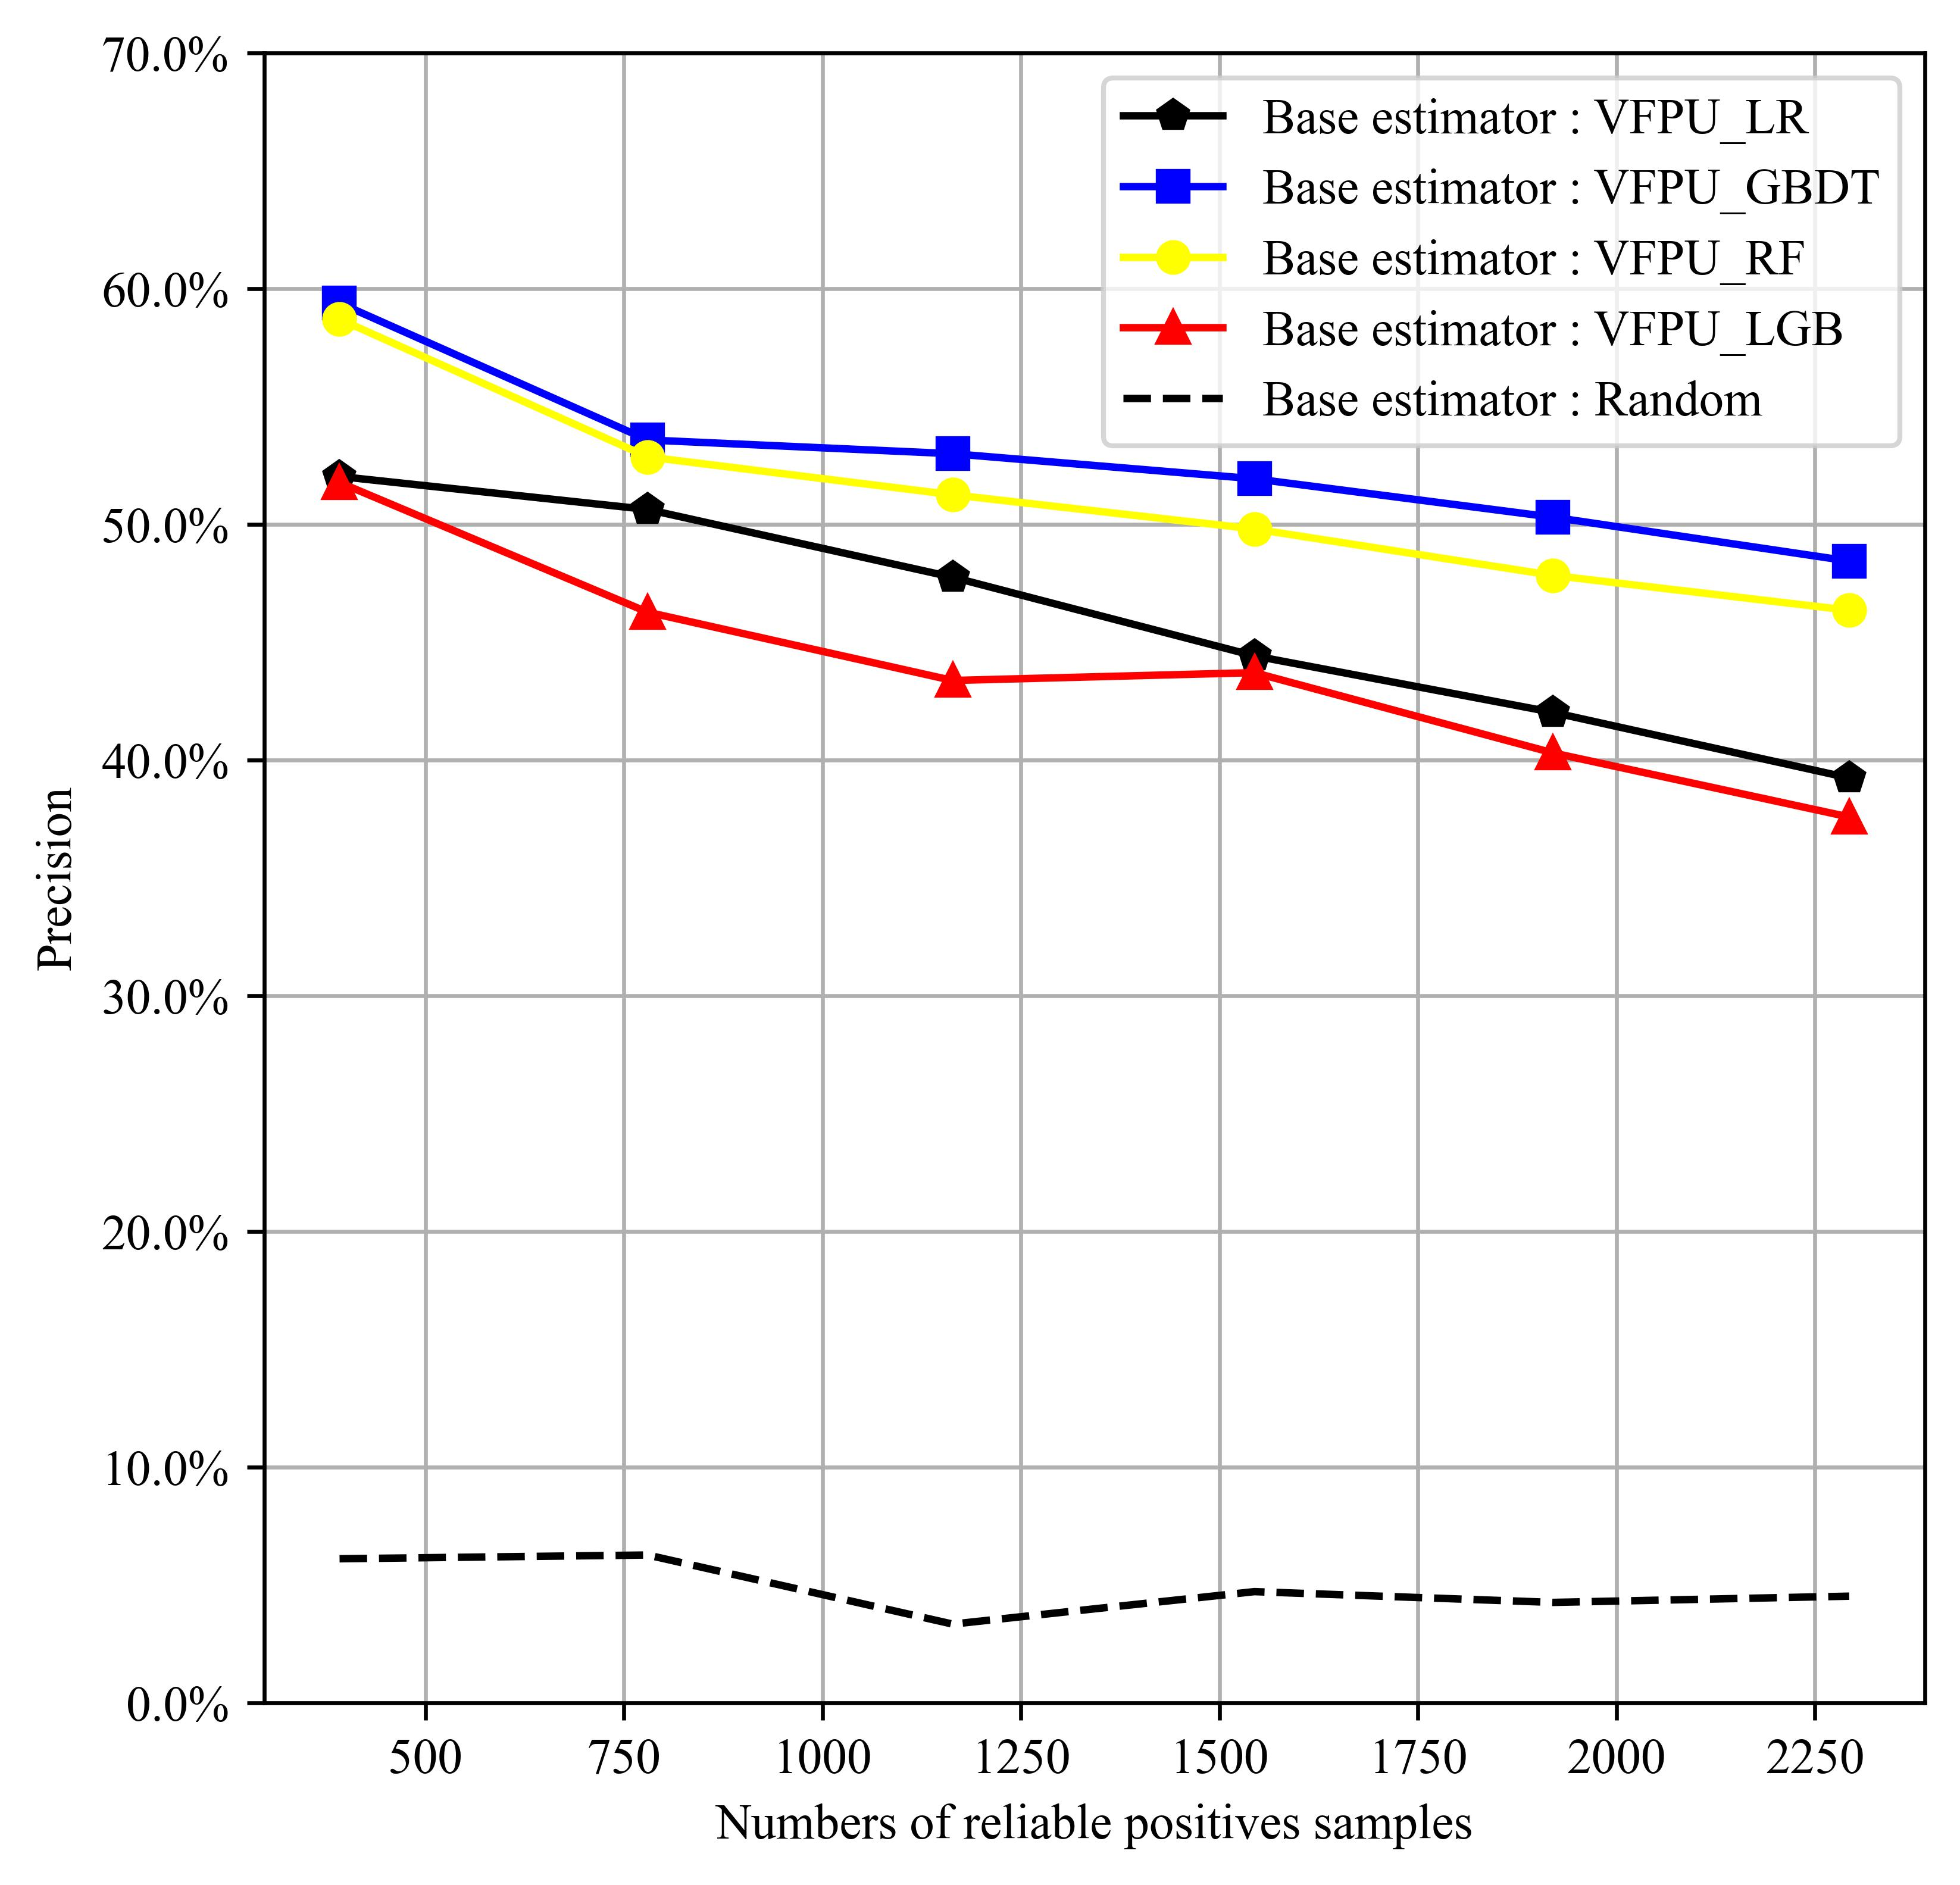
\includegraphics[width=0.45\textwidth,height=4.1cm]{chapters/imgs/Figure 2 (1) in JEPG format}}
	\subfigure[]{\label{RQ2.1.sub2}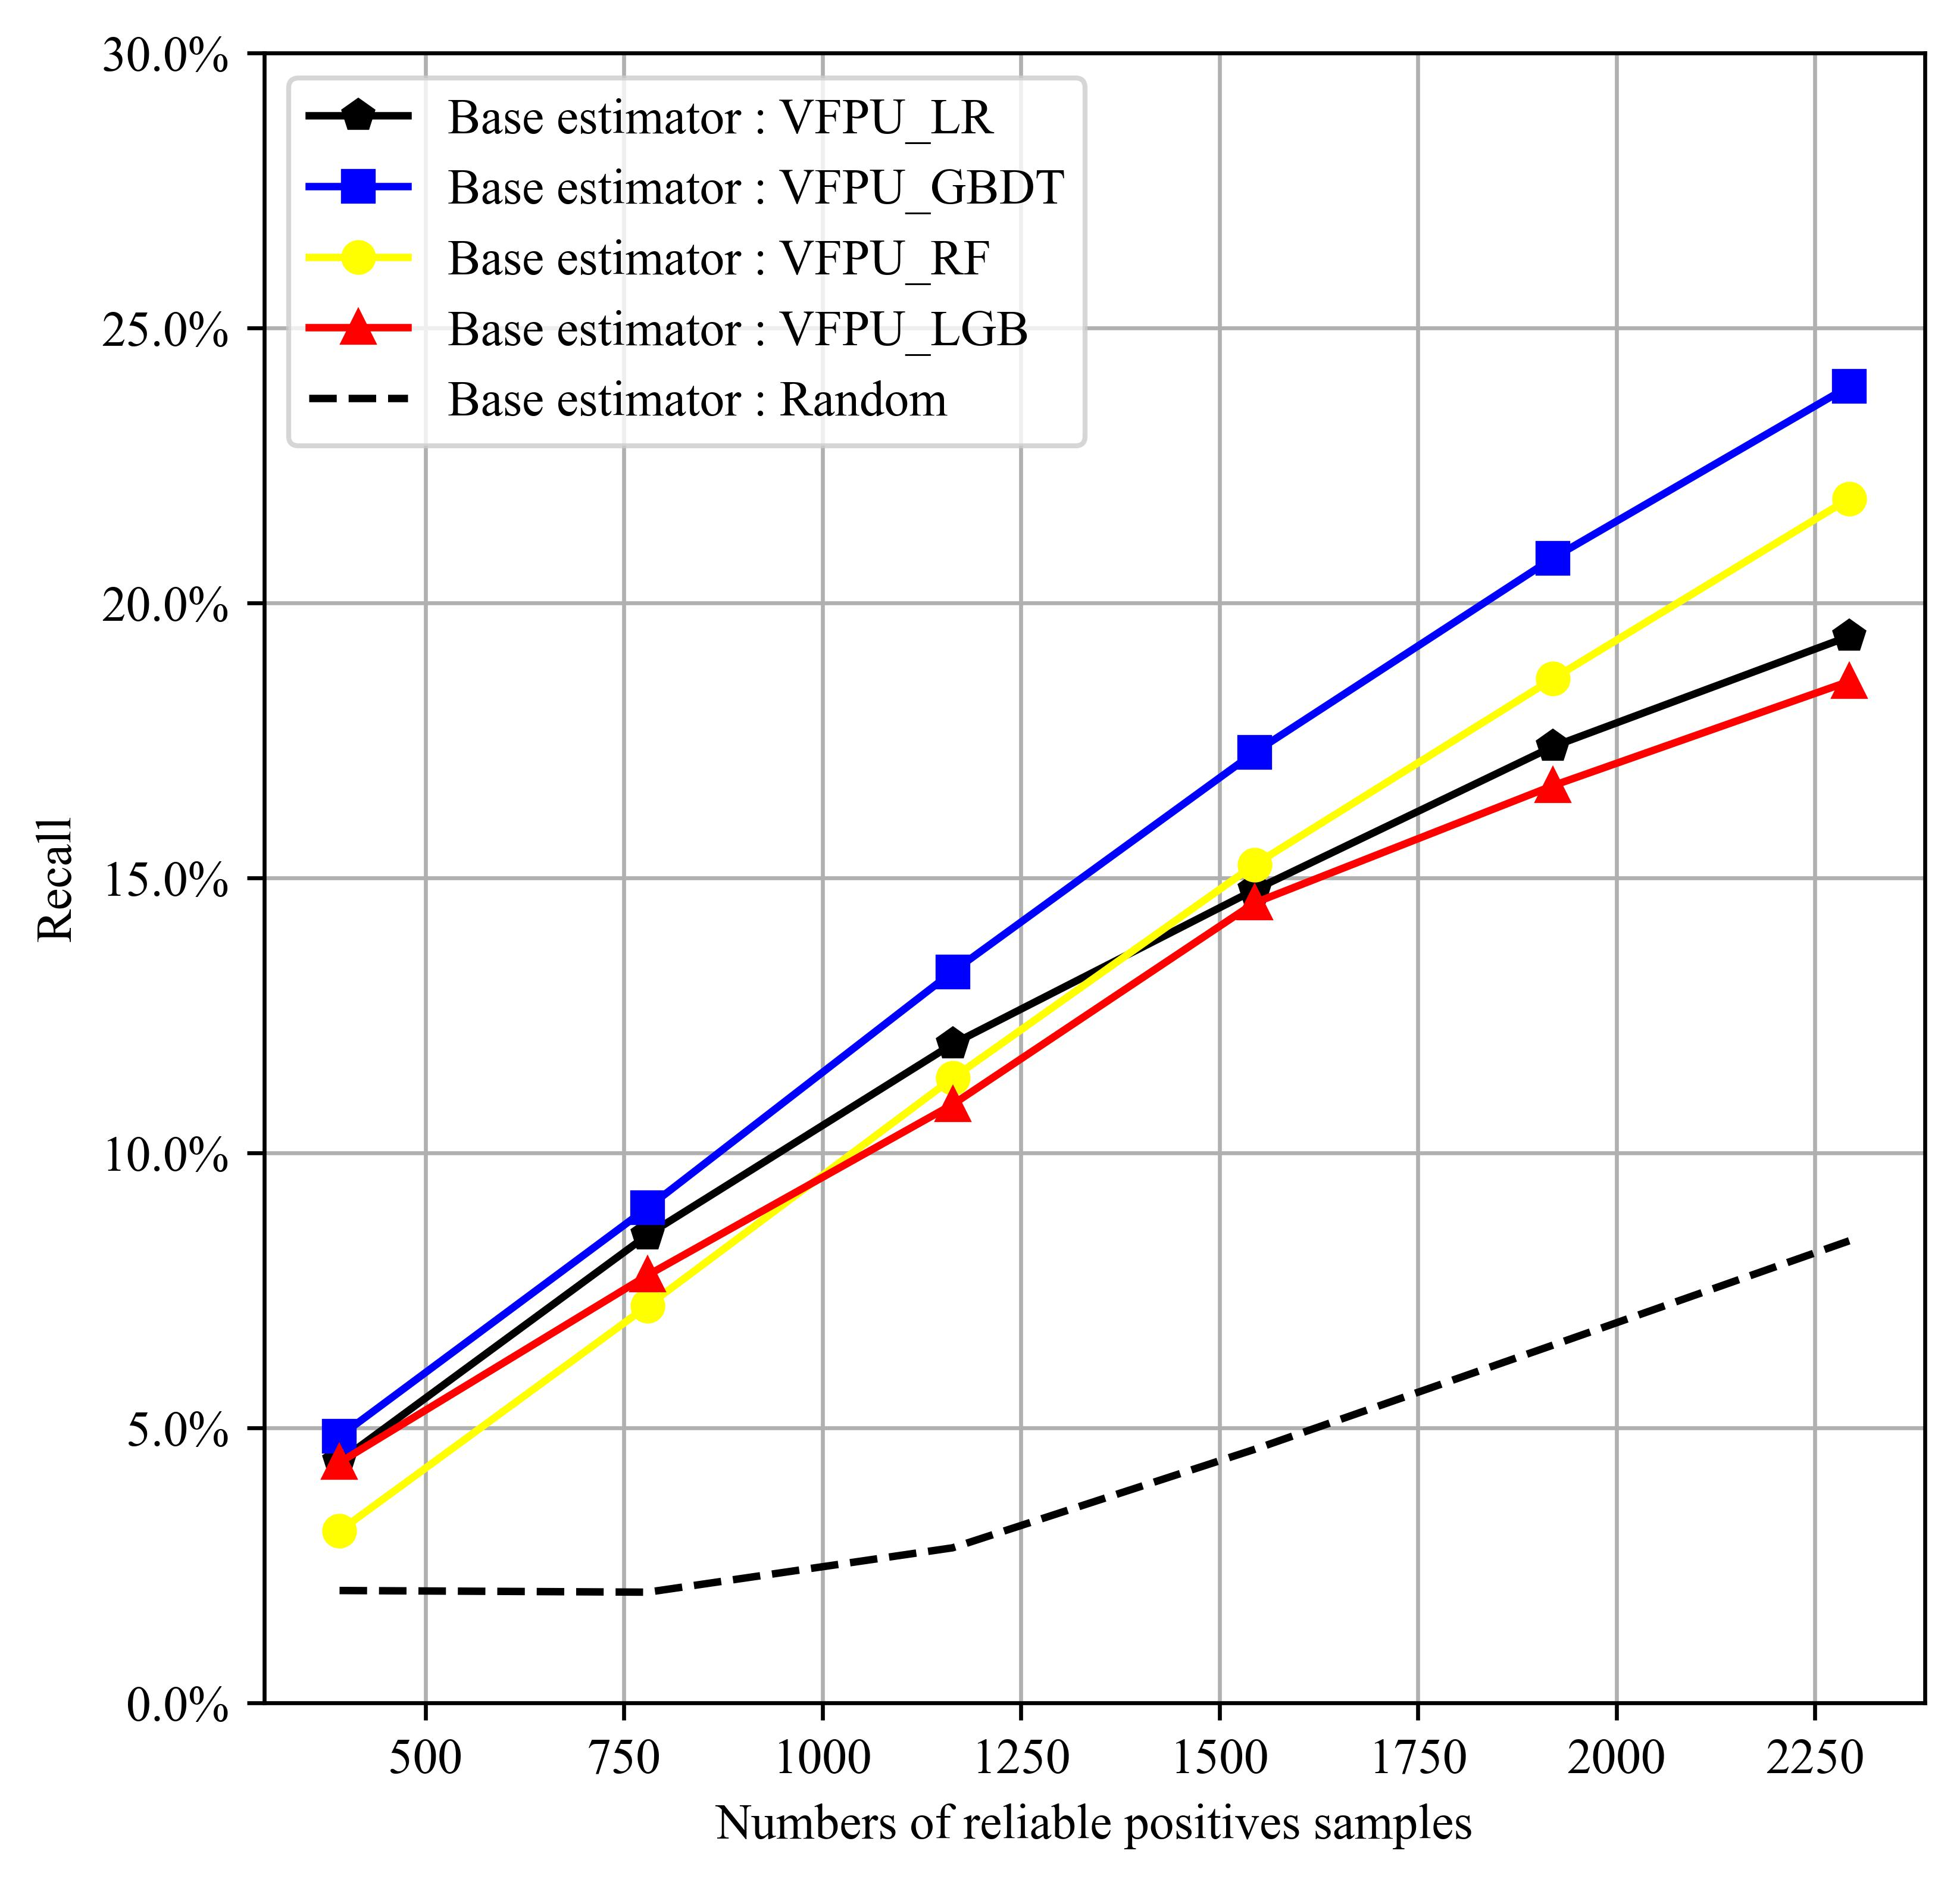
\includegraphics[width=0.45\textwidth,height=4.1cm]{chapters/imgs/Figure 2 (2) in JEPG format}}
	\subfigure[]{\label{RQ2.1.sub3}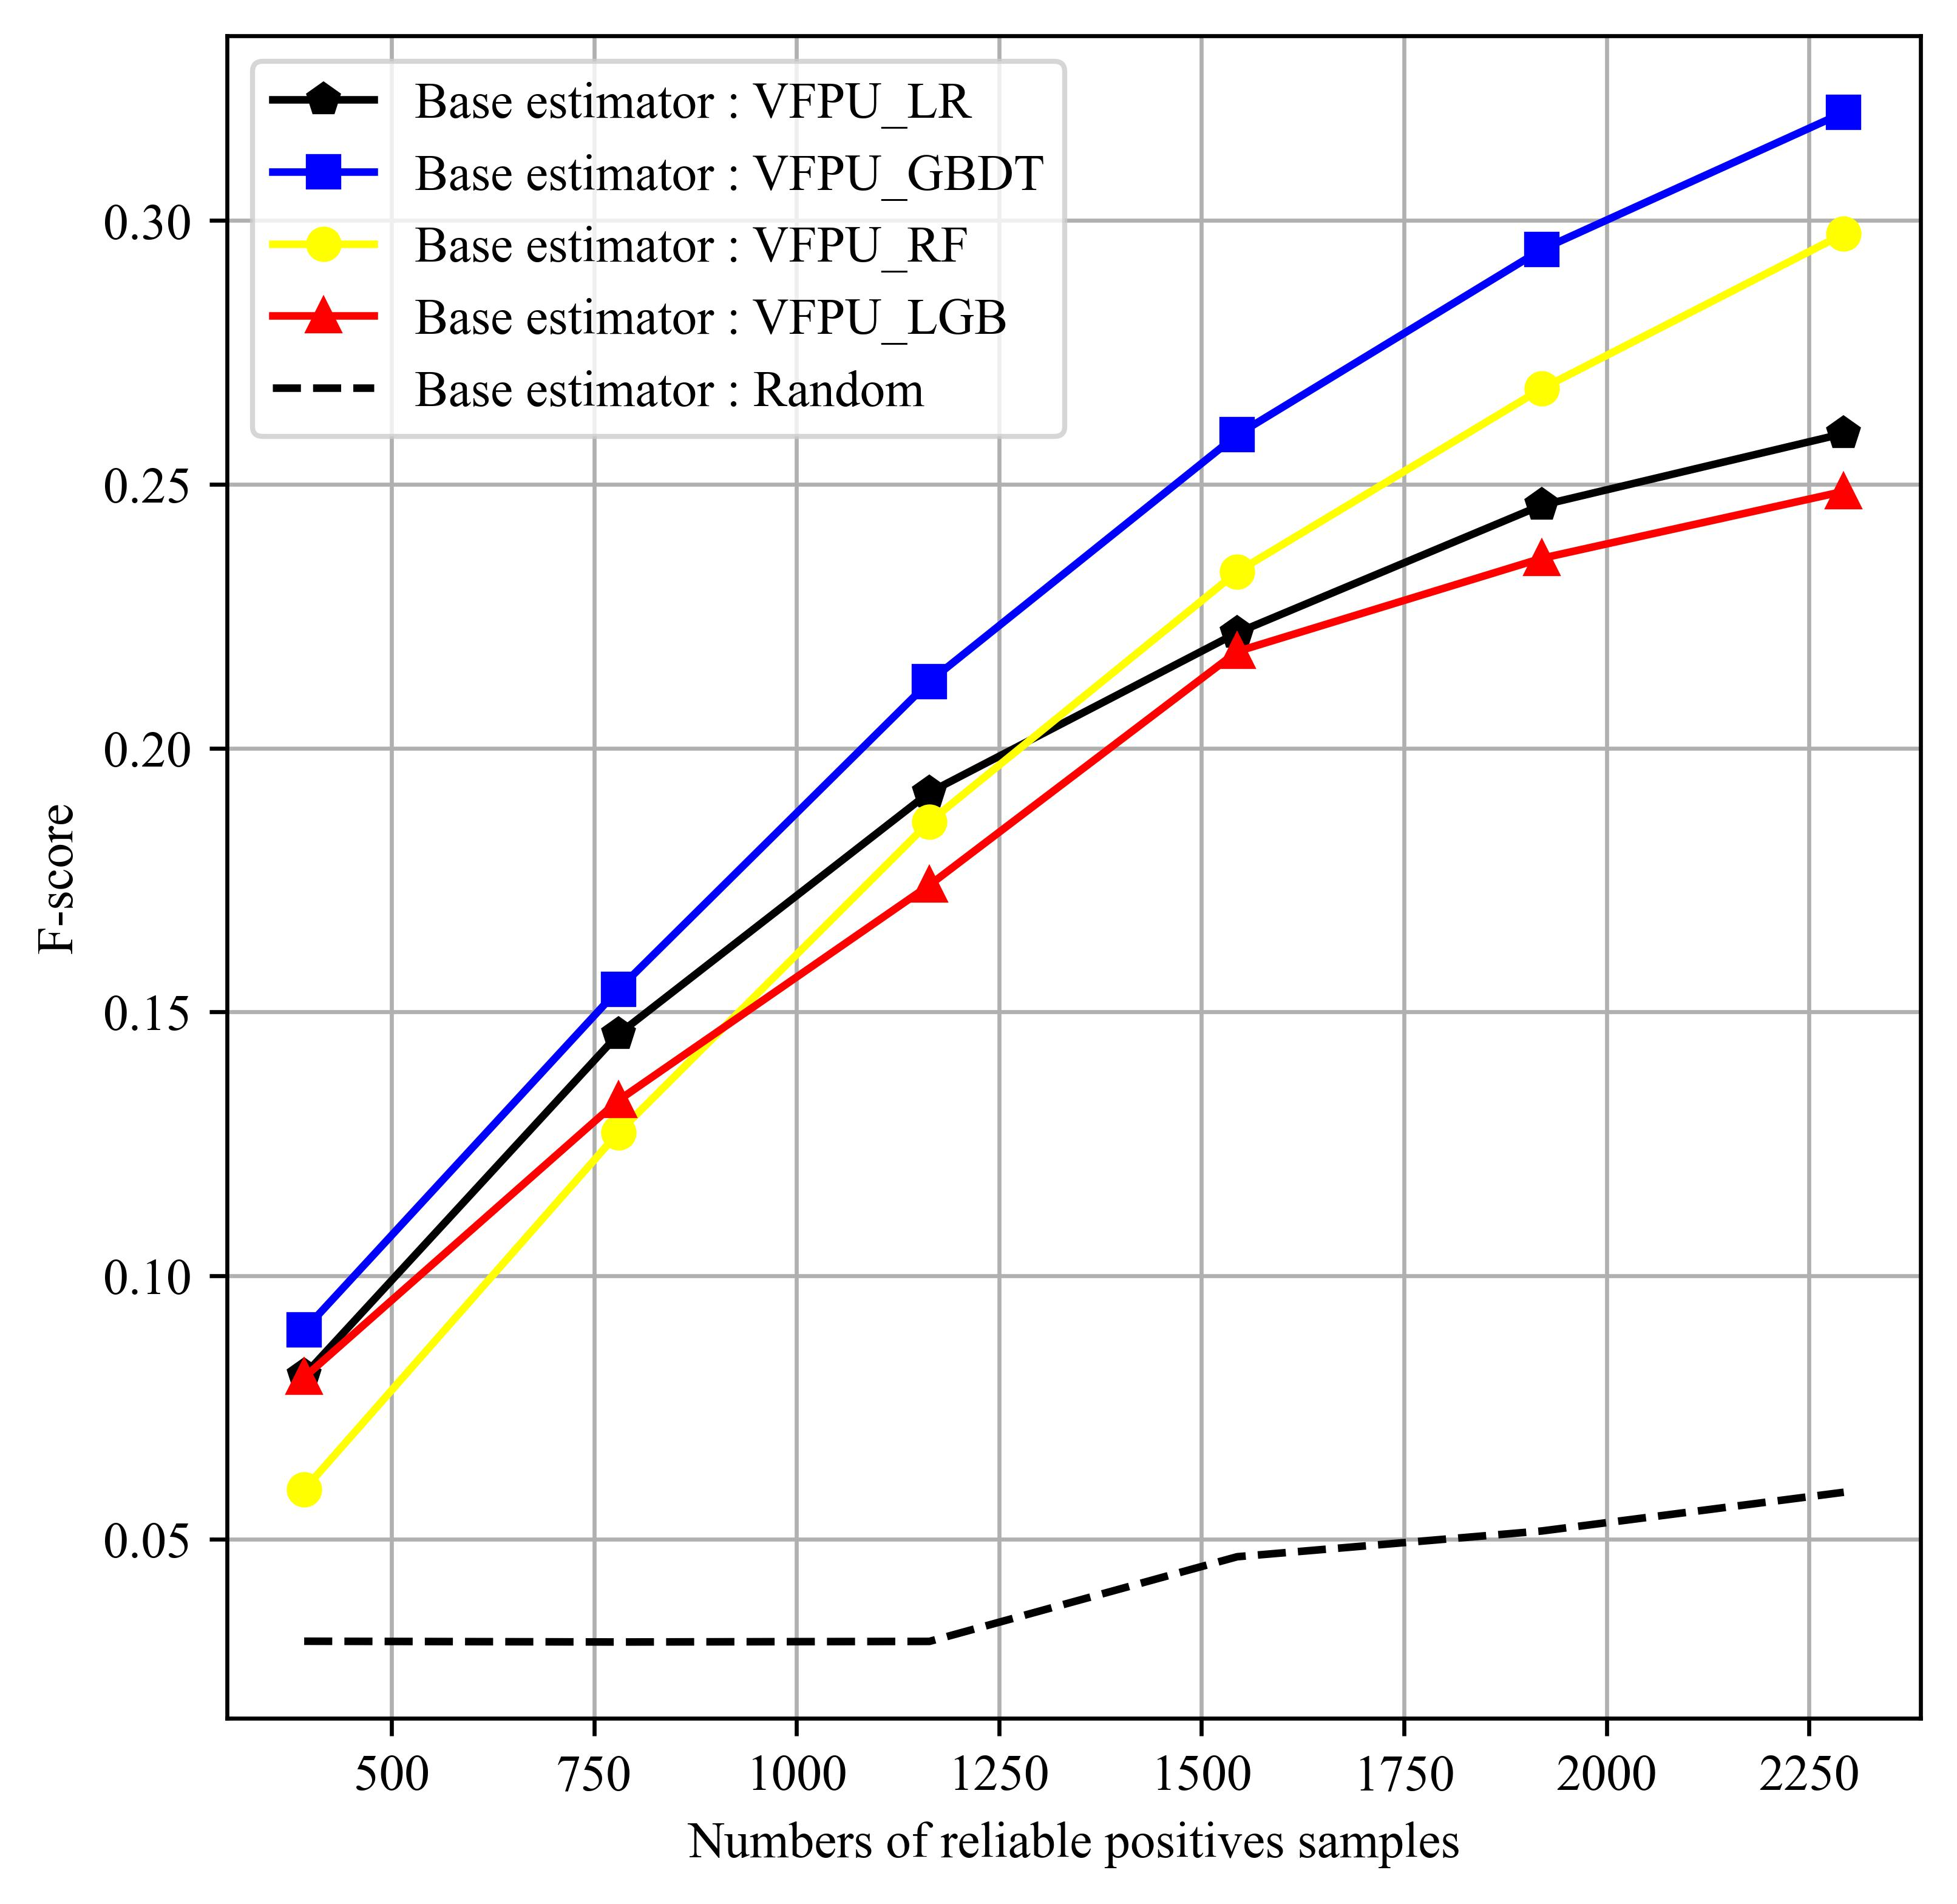
\includegraphics[width=0.45\textwidth,height=4.1cm]{chapters/imgs/Figure 2 (3) in JEPG format}}
	\subfigure[]{\label{RQ2.1.sub4}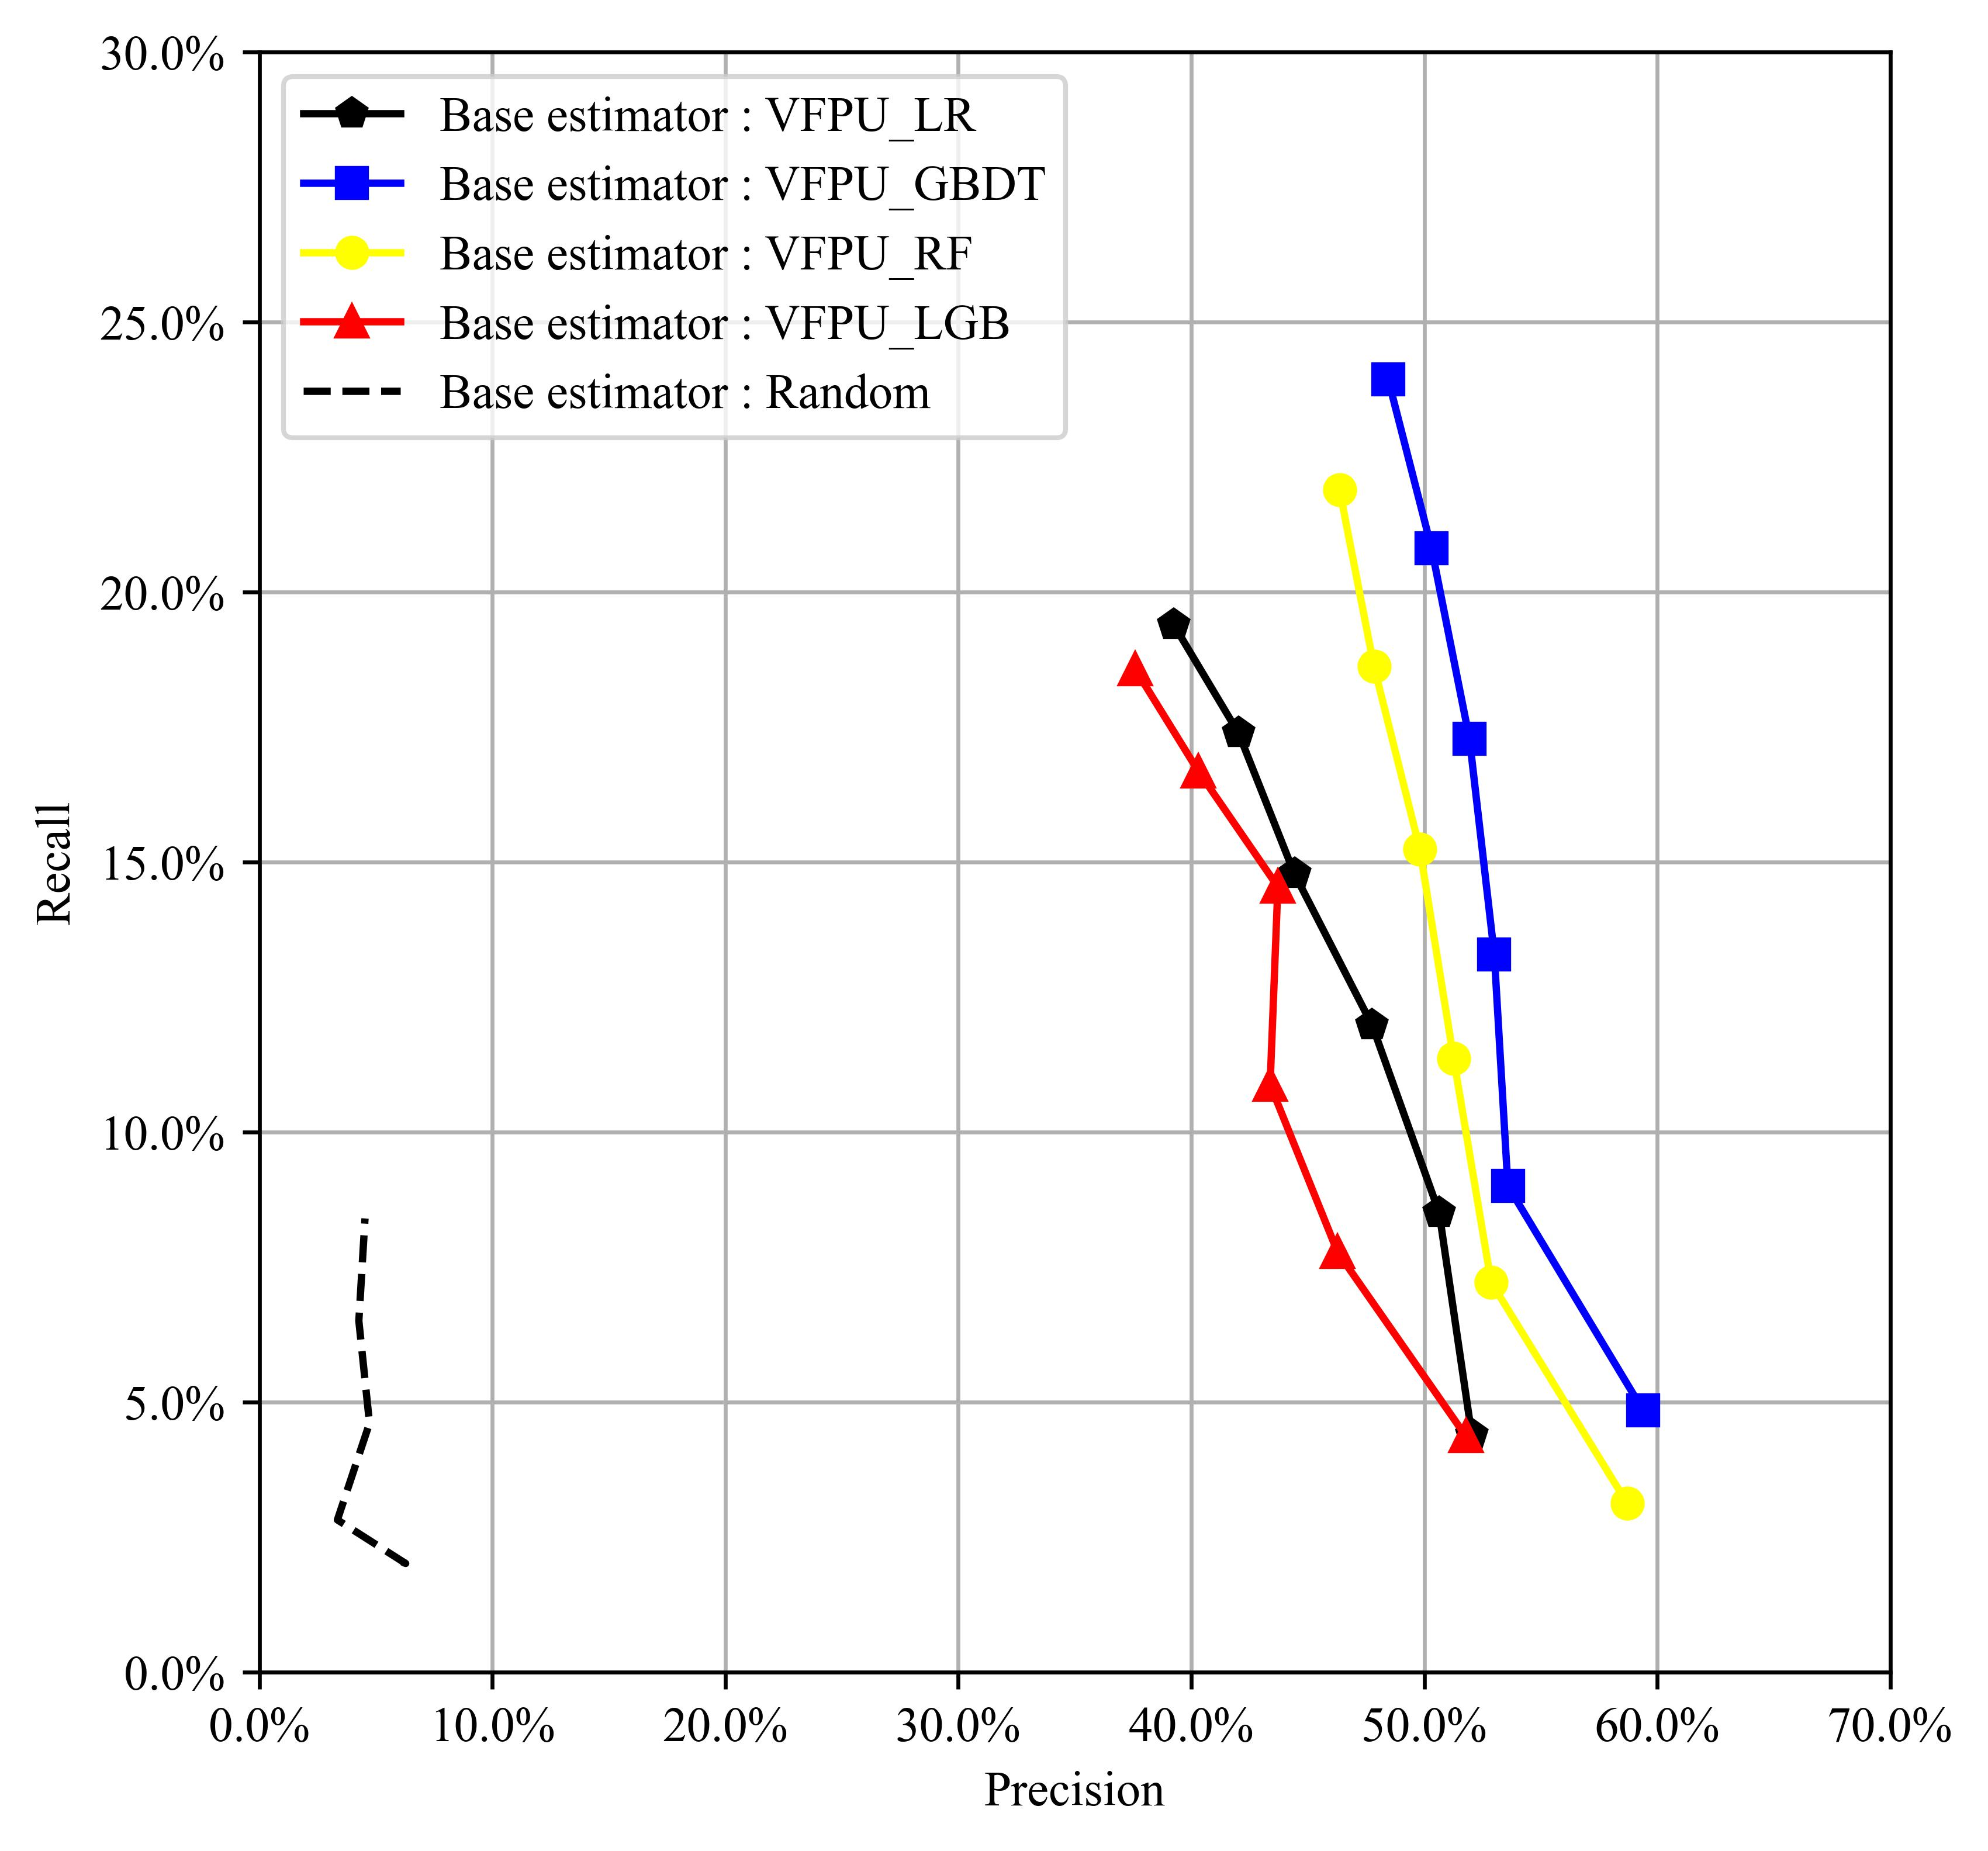
\includegraphics[width=0.45\textwidth,height=4.1cm]{chapters/imgs/Figure 2 (4) in JEPG format}}
	\bicaption[\xiaosi 不同基学器在不同可靠正样本数量下的性能]
	{\centering \songti \wuhao 不同基学器的性能:(a)精度;(b)召回率;(c)F-score;(d)精度-召回率(Bank)}
	{\centering \wuhao Base estimators performance: (a) Precision; (b) Recall; (c) F-score; (d) Precision-Recall}
	\label{RQ2.1}
\end{figure}

\vspace{-0.5cm} 


\begin{figure}[H]
	\centering
	\subfigure[]{\label{RQ2.2.sub1}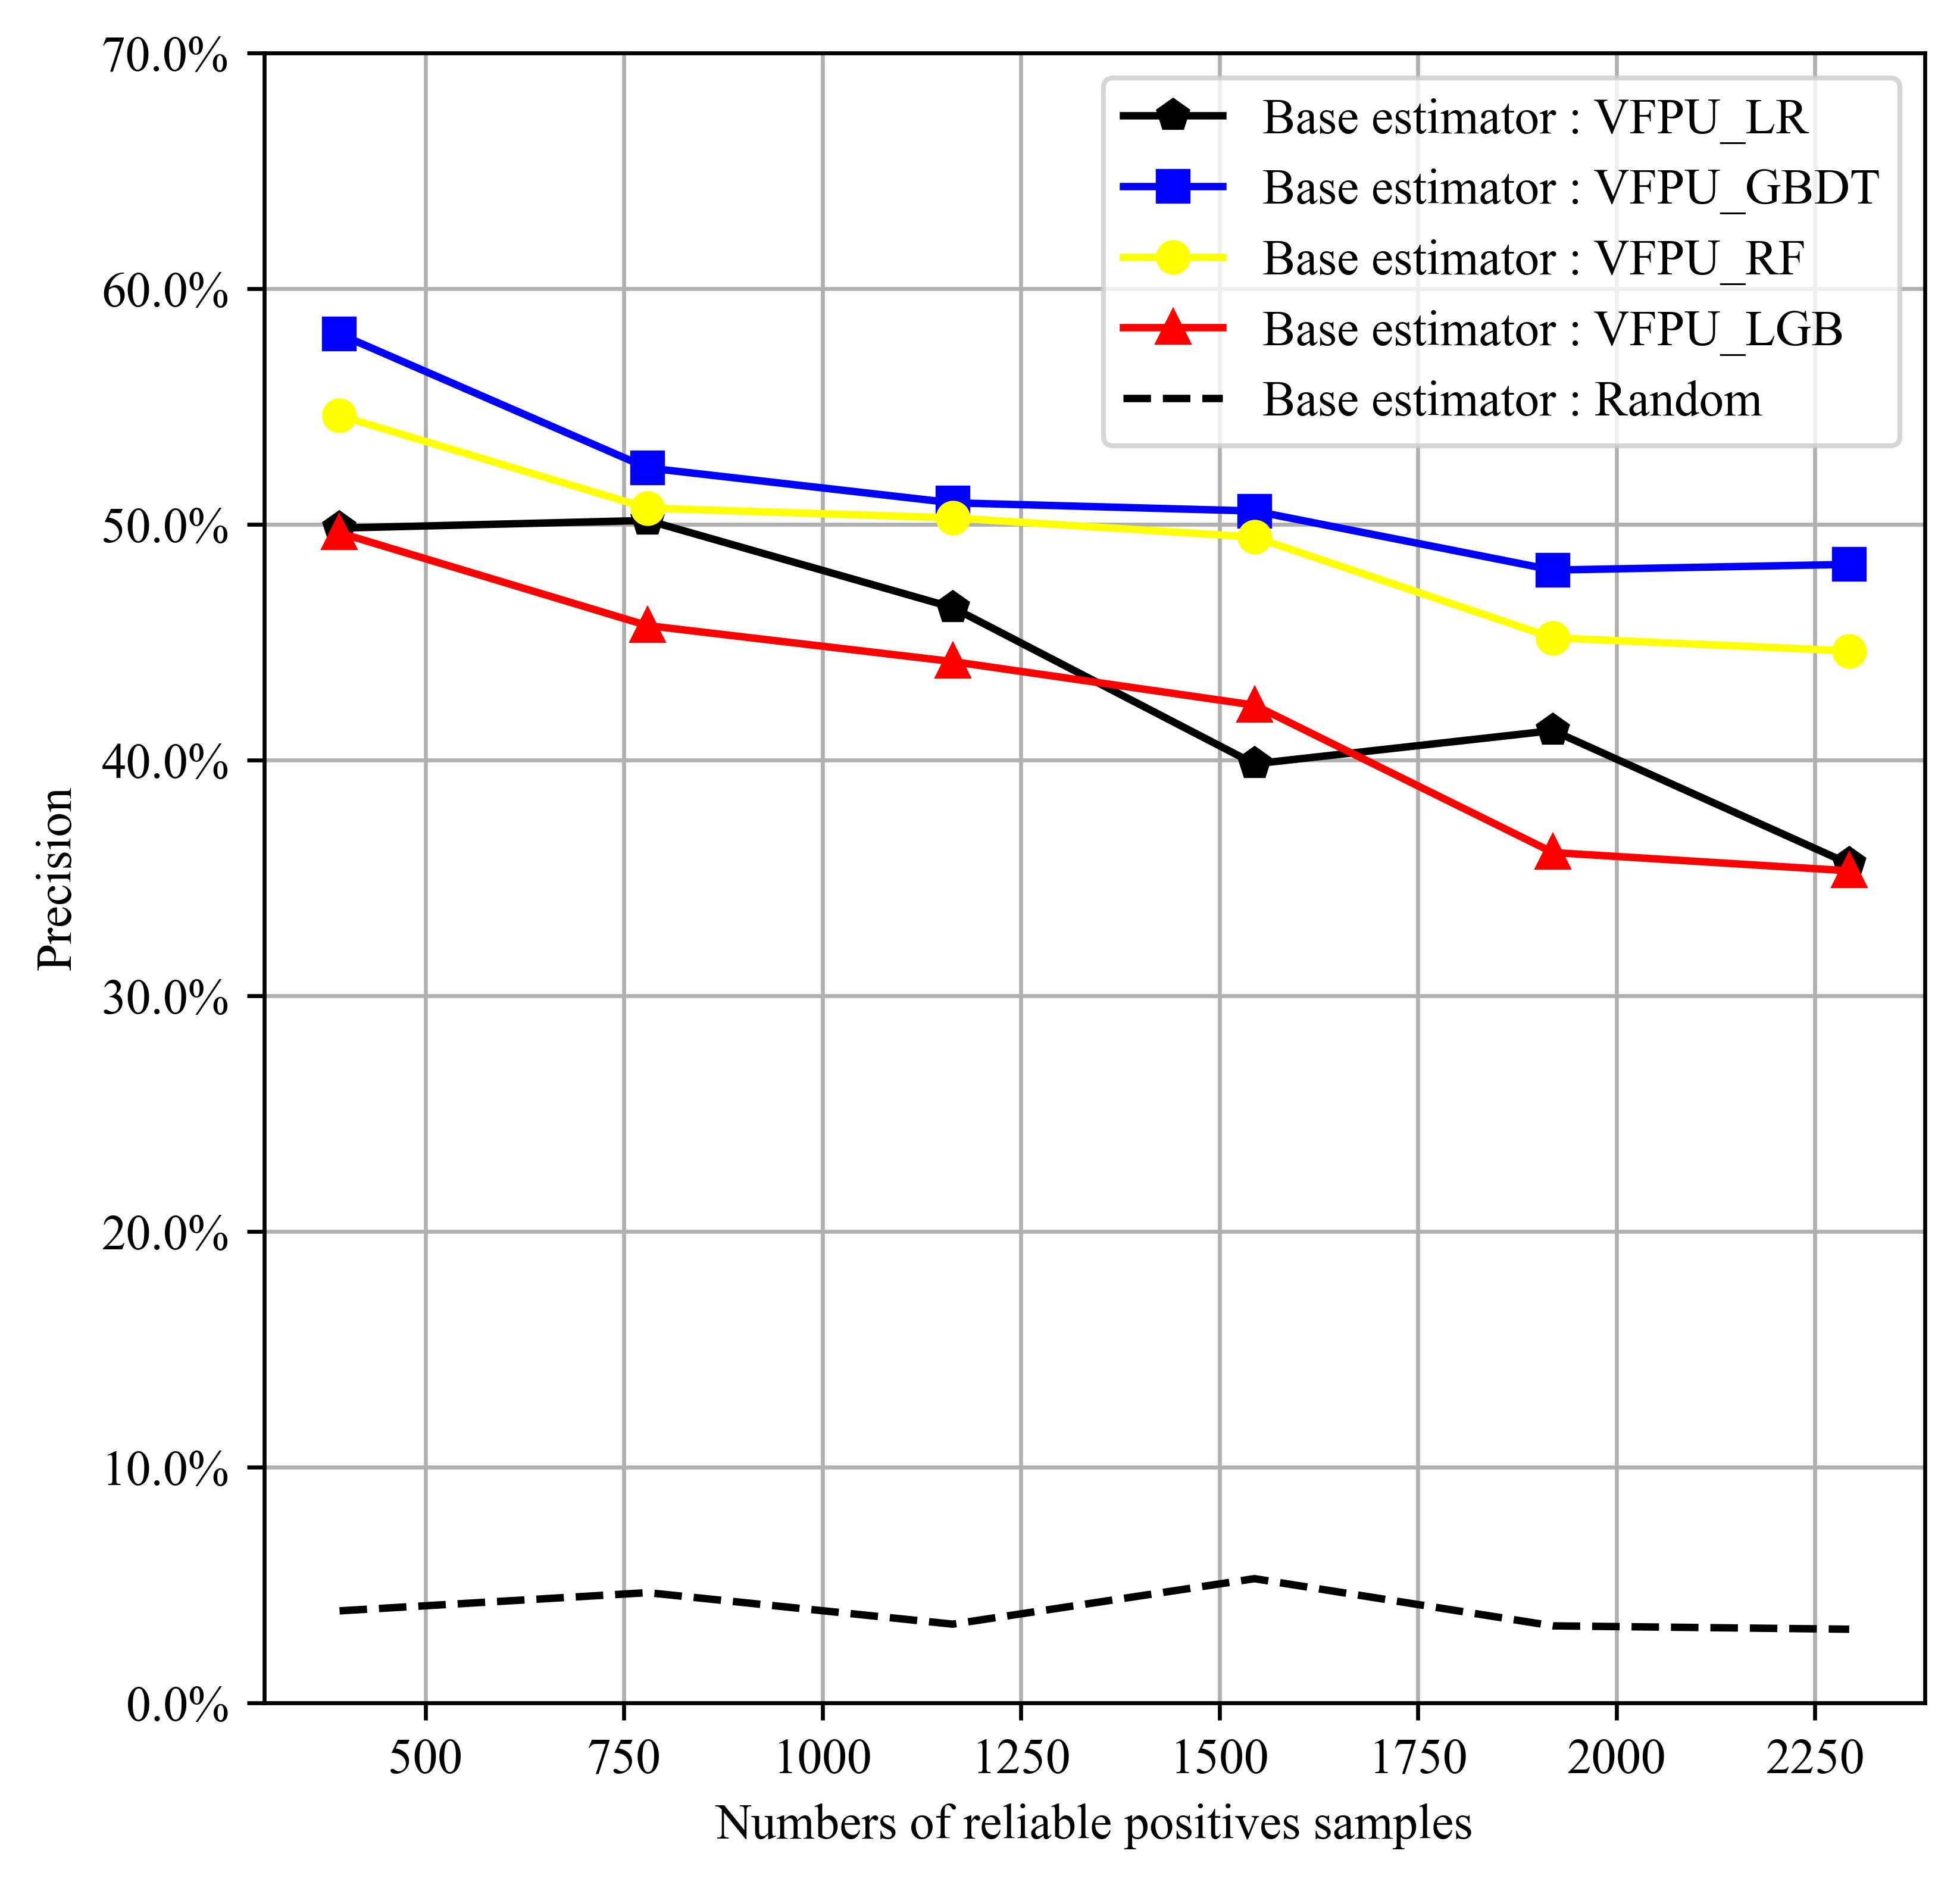
\includegraphics[width=0.45\textwidth,height=4.1cm]{chapters/imgs/Figure 3 (1) in JEPG format}}
	\subfigure[]{\label{RQ2.2.sub2}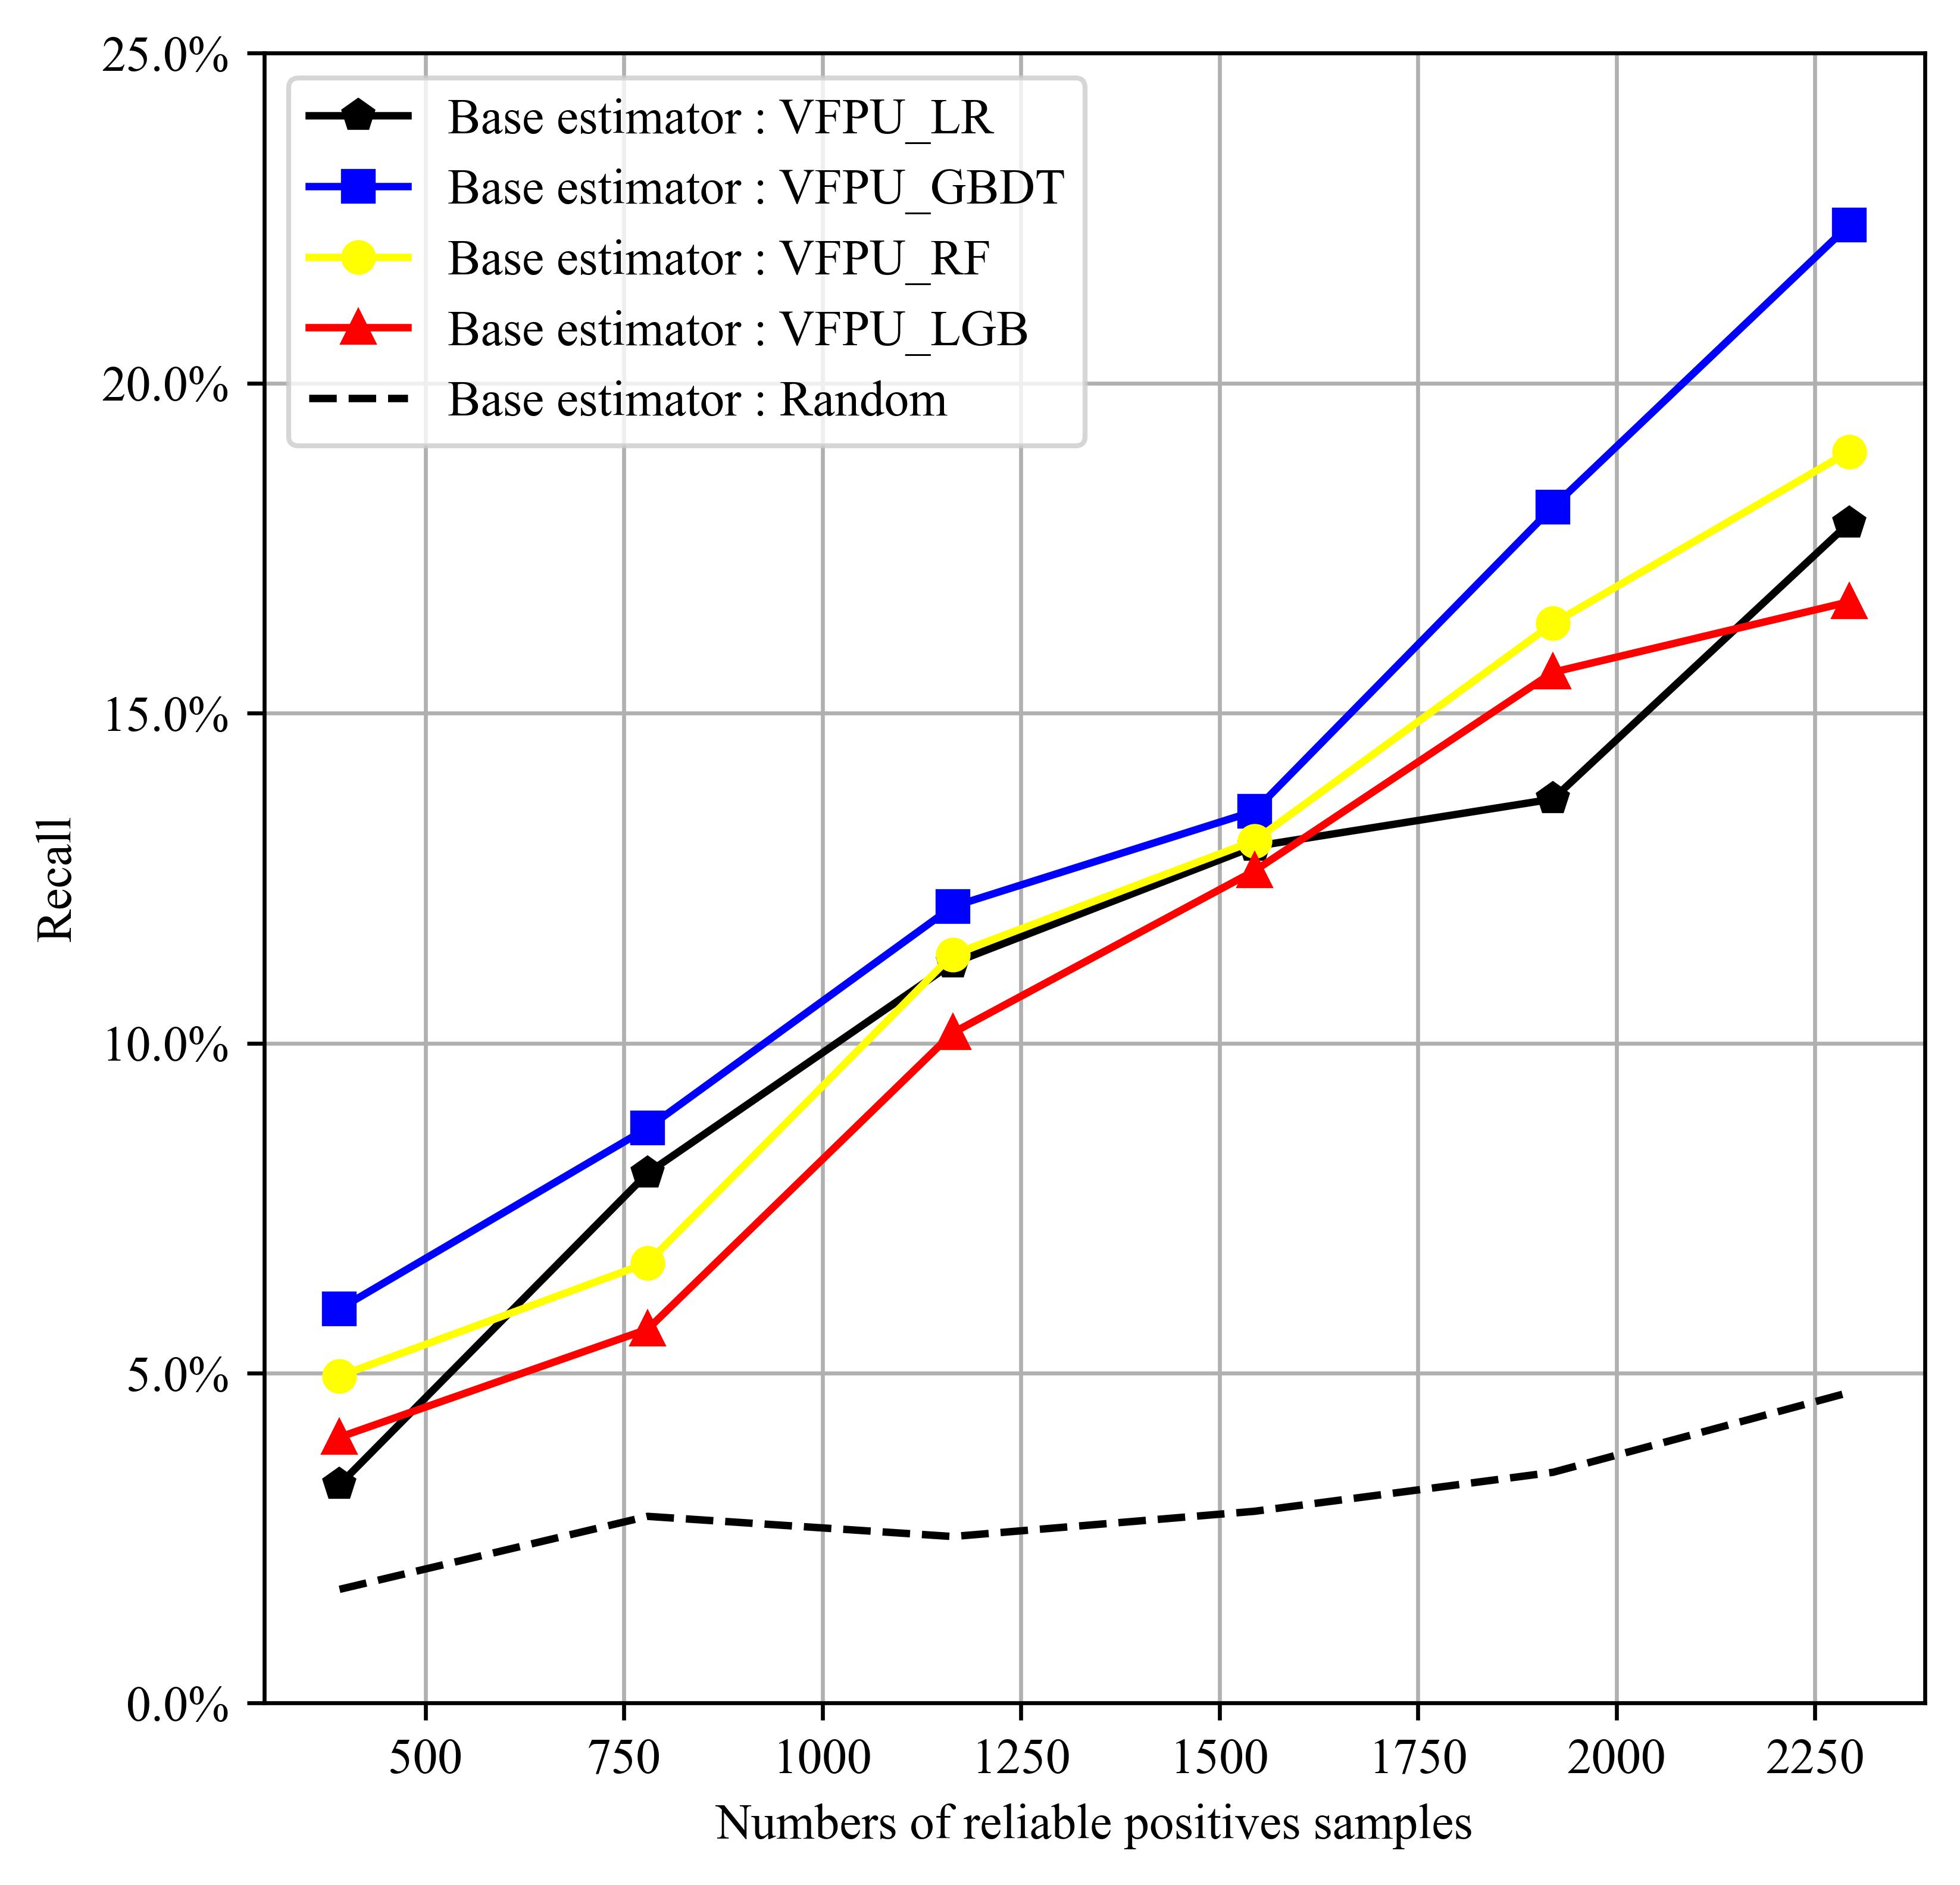
\includegraphics[width=0.45\textwidth,height=4.1cm]{chapters/imgs/Figure 3 (2) in JEPG format}}
	\subfigure[]{\label{RQ2.2.sub3}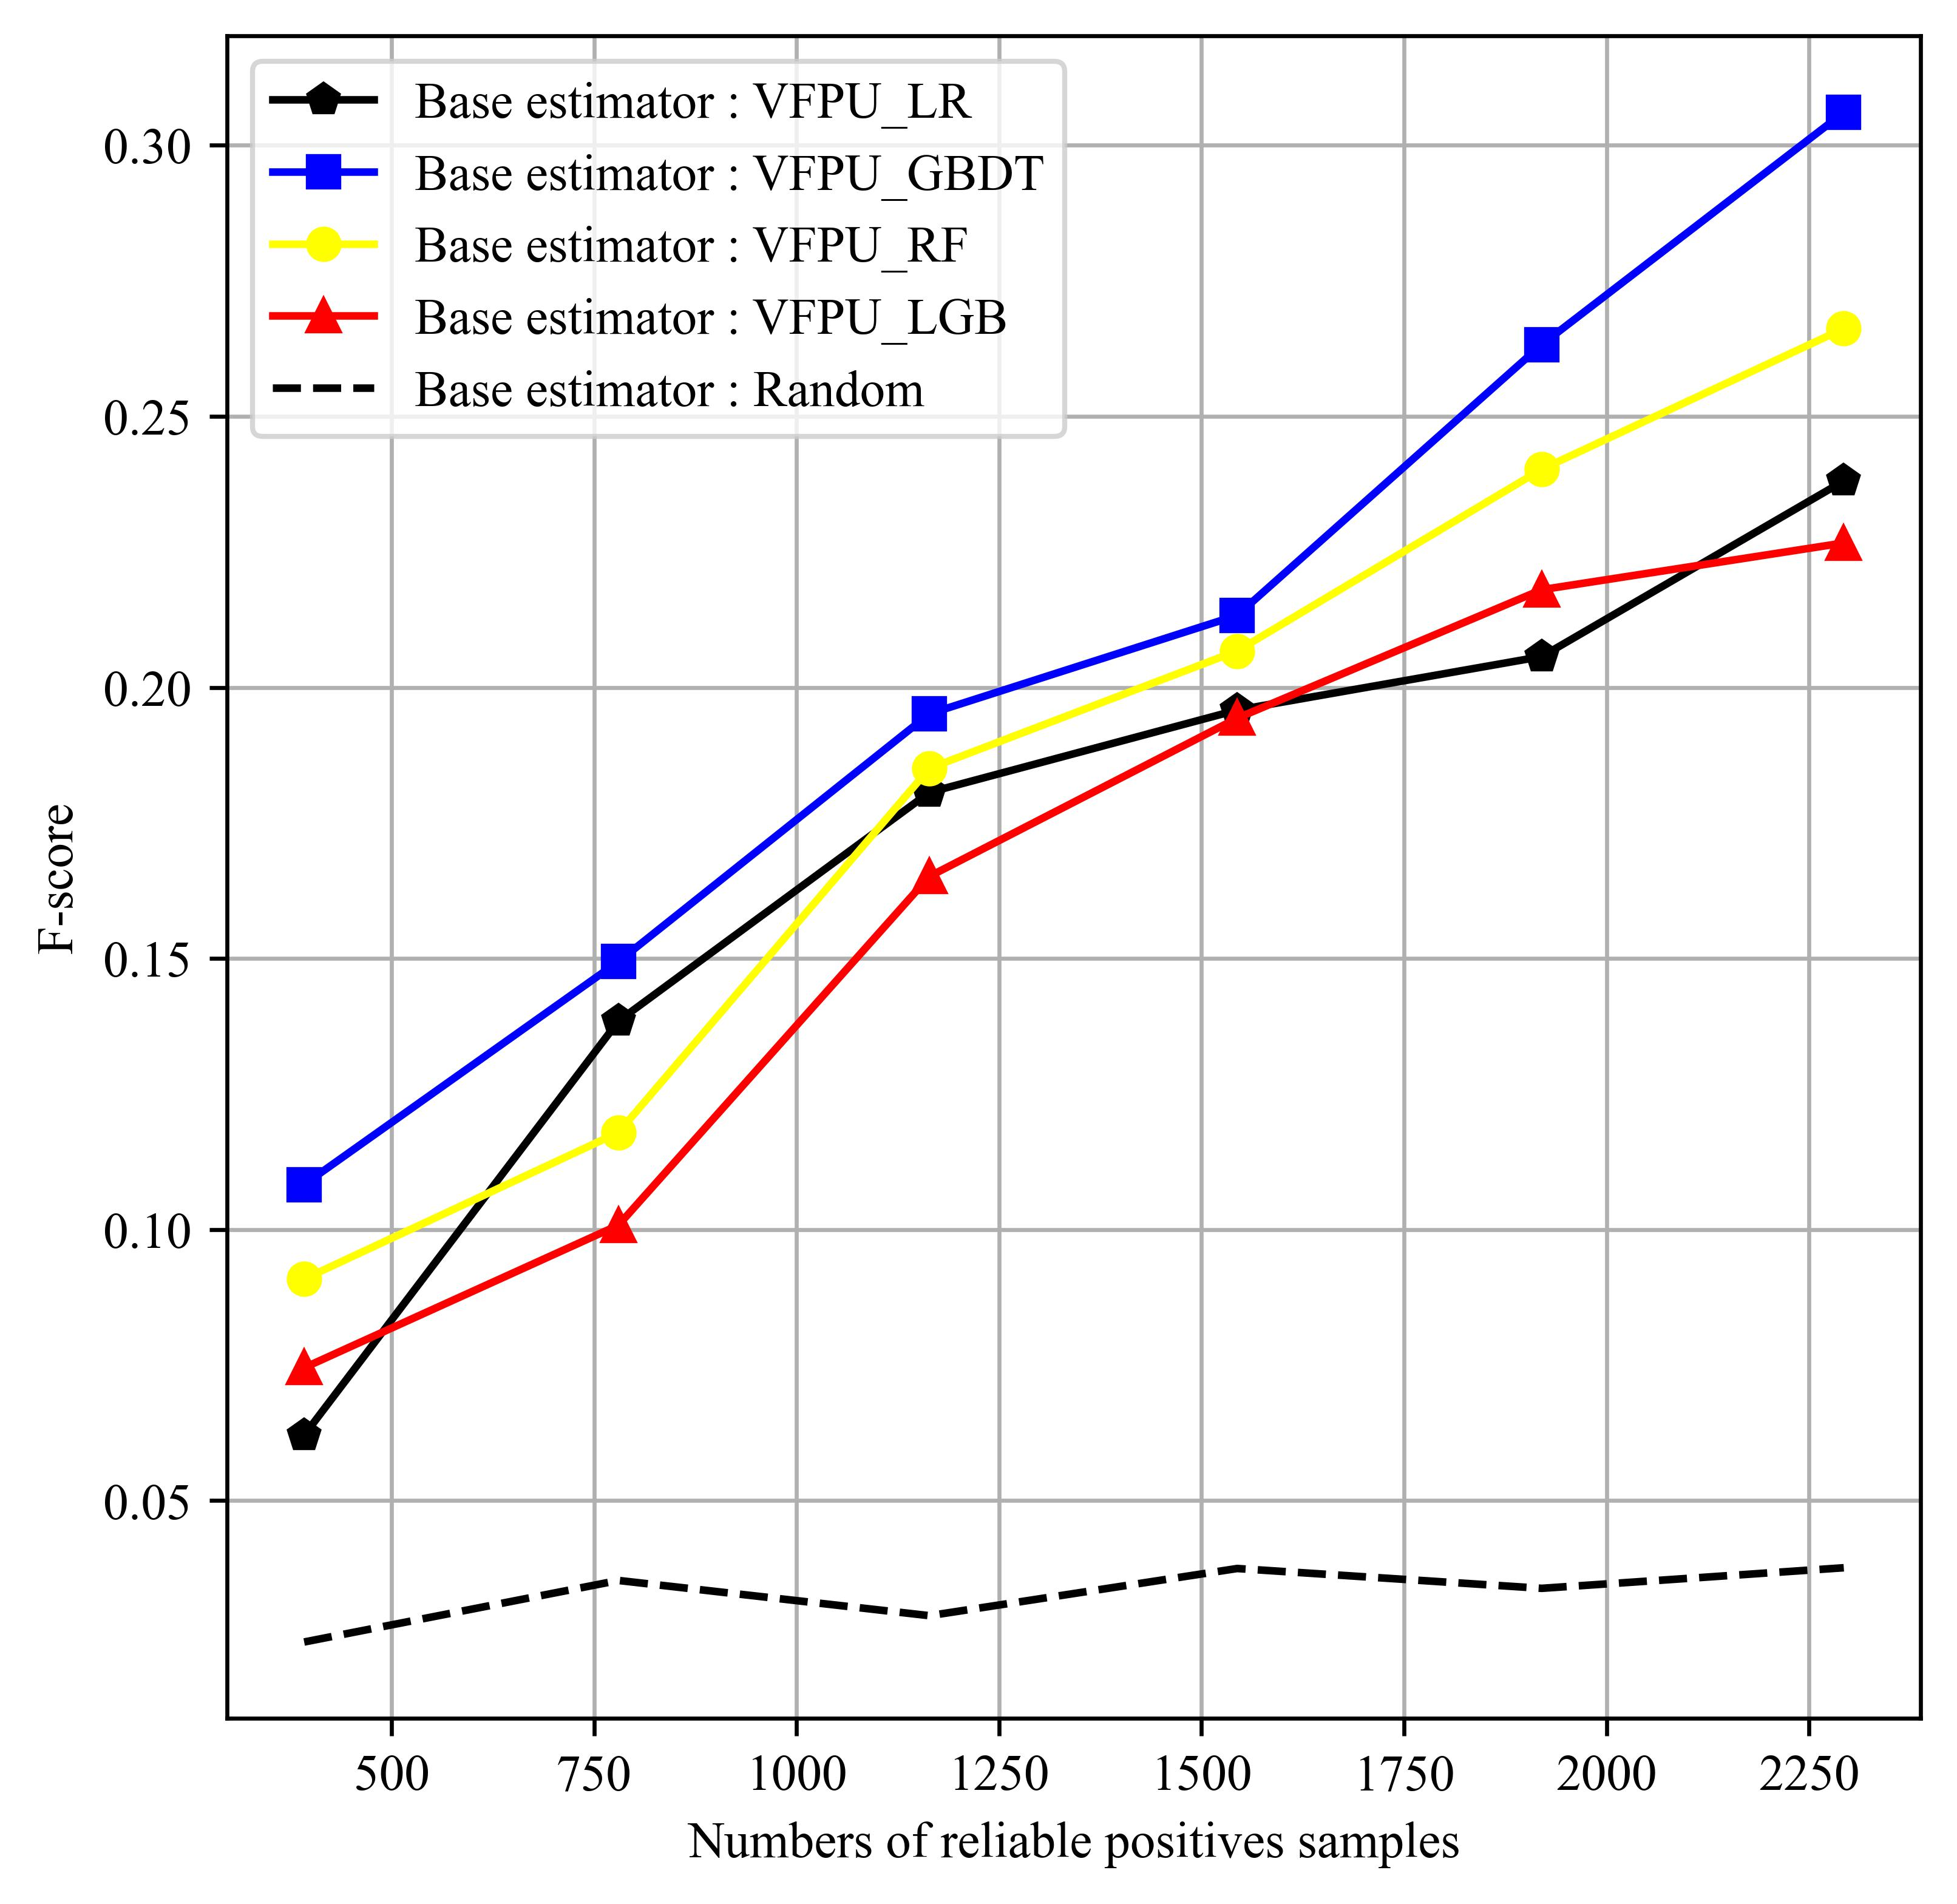
\includegraphics[width=0.45\textwidth,height=4.1cm]{chapters/imgs/Figure 3 (3) in JEPG format}}
	\subfigure[]{\label{RQ2.2.sub4}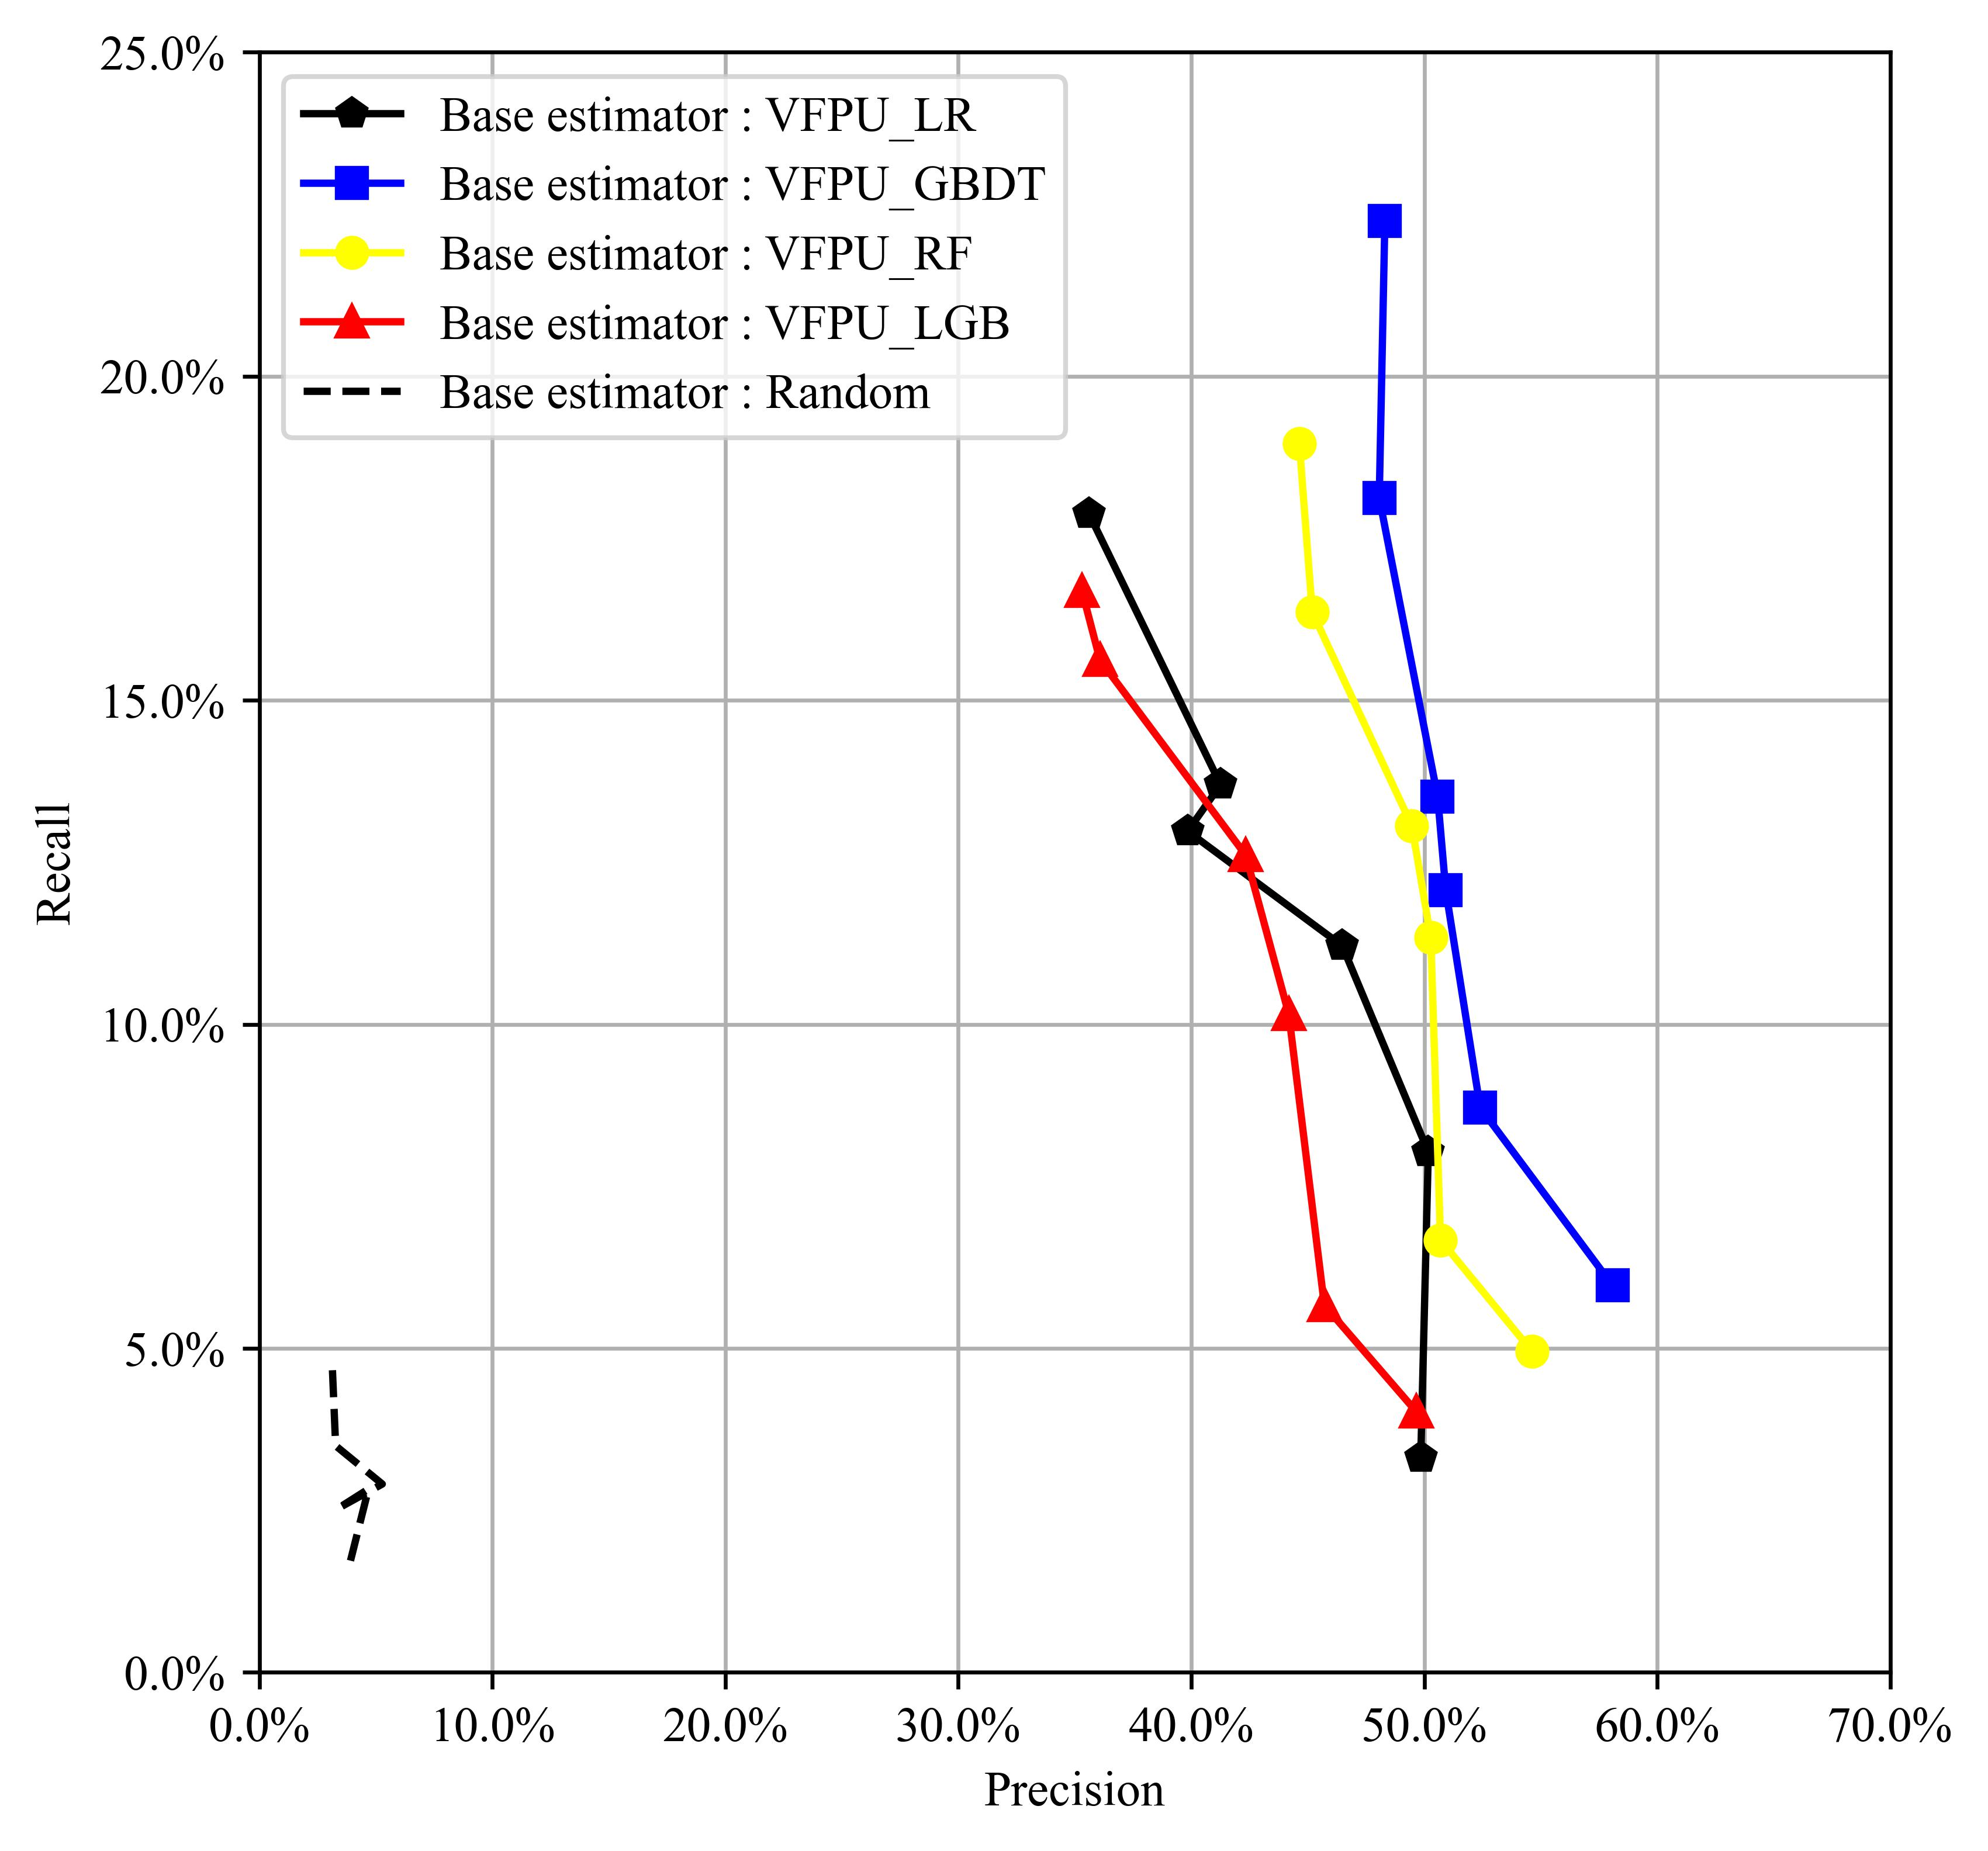
\includegraphics[width=0.45\textwidth,height=4.1cm]{chapters/imgs/Figure 3 (4) in JEPG format}}
	
	\bicaption[\xiaosi 不同基学器在不同可靠正样本数量下的性能]
	{\centering \songti \wuhao 不同基学器的性能:(a)精度;(b)召回率;(c)F-score;(d)精度-召回率(Credit)}
	{\centering \wuhao Base estimators performance: (a) Precision; (b) Recall; (c) F-score; (d) Precision-Recall}
	\label{RQ2.2}
\end{figure}

尽管VFPU\_RF学习器在某些情况下显示出相对可比较的精确度,但随着可靠样本数量的增加,其性能(特别是在召回率和F-score方面)下降得更快。相比之下,VFPU\_LR和VFPU\_LGB模型虽然在不同样本大小下表现稳定,但并未达到VFPU\_GBDT在精确度和召回率方面表现出的整体性能。因此,图 \ref{RQ2.1.sub1} 清楚地表明,VFPU\_GBDT不仅提供了更高的精确度,而且在召回率之间保持了平衡的权衡,从而在评估的模型中实现了最高的F-score。



\vspace{-0.1cm}
\begin{figure}[h]
	\centering
	\subfigure[]{\label{RQ2.3.sub1}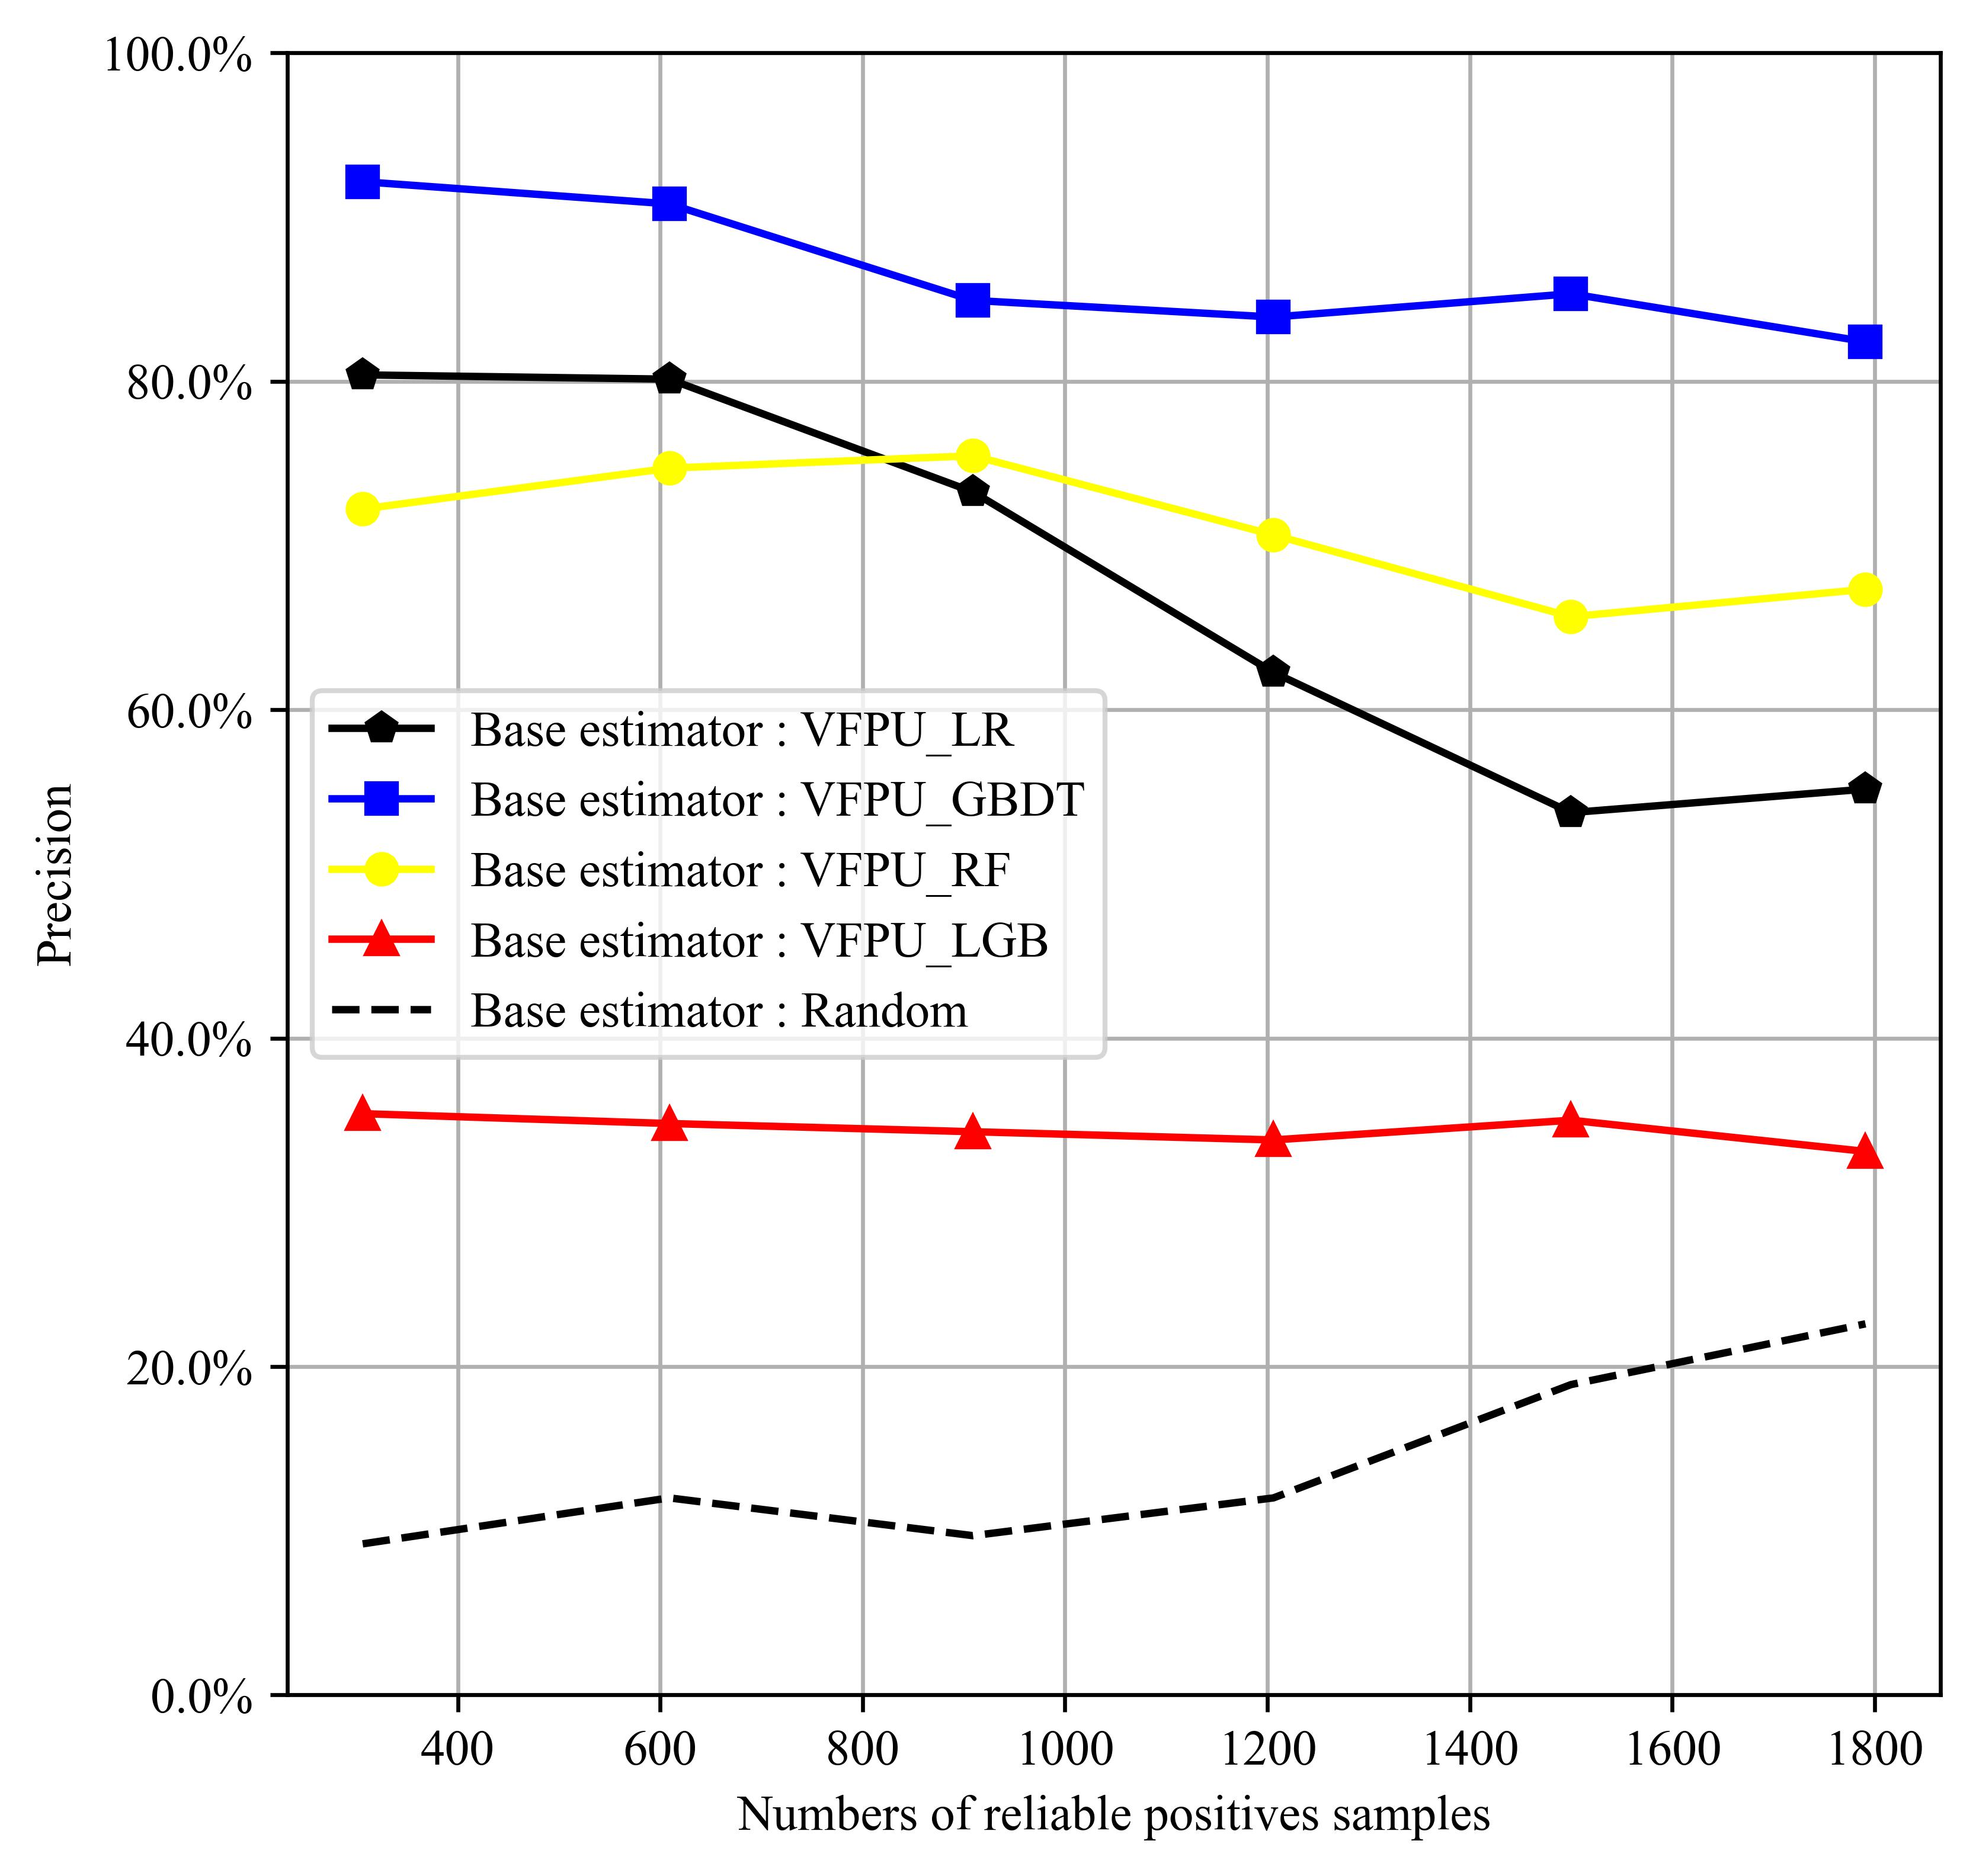
\includegraphics[width=0.45\textwidth,height=4.1cm]{chapters/imgs/Figure 4 (1) in JEPG format}}
	\subfigure[]{\label{RQ2.3.sub2}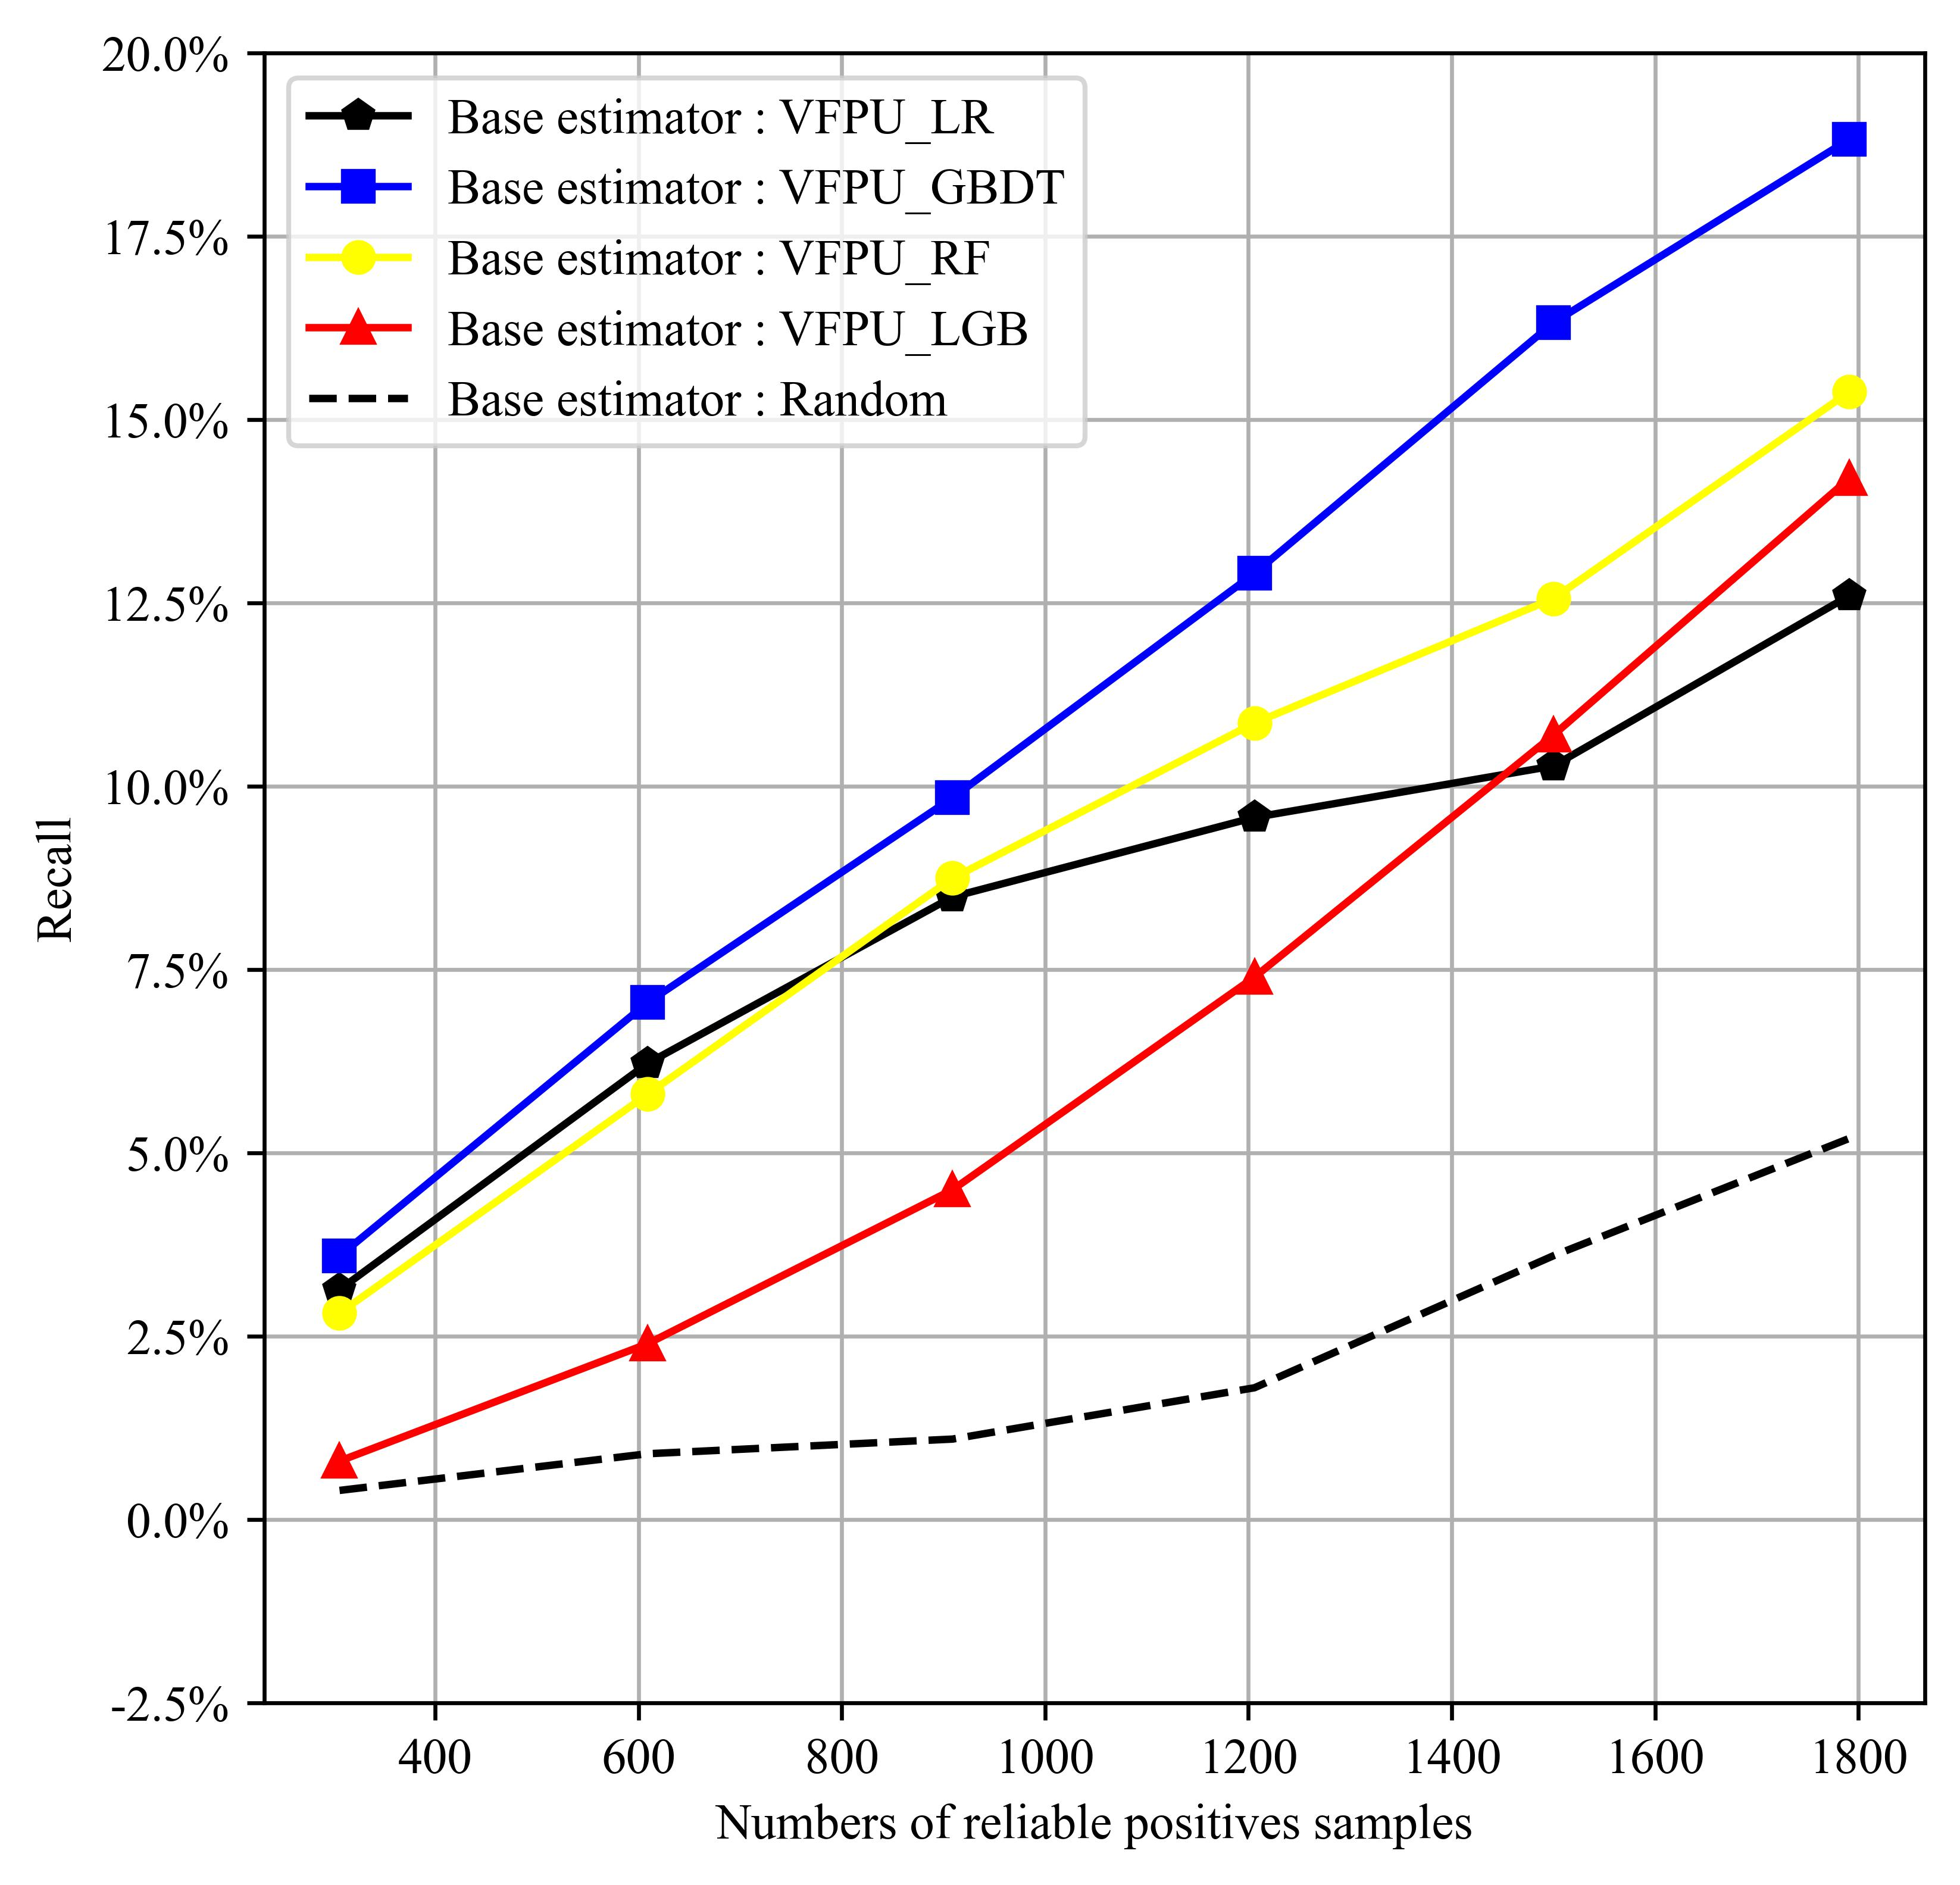
\includegraphics[width=0.45\textwidth,height=4.1cm]{chapters/imgs/Figure 4 (2) in JEPG format}}
	\subfigure[]{\label{RQ2.3.sub3}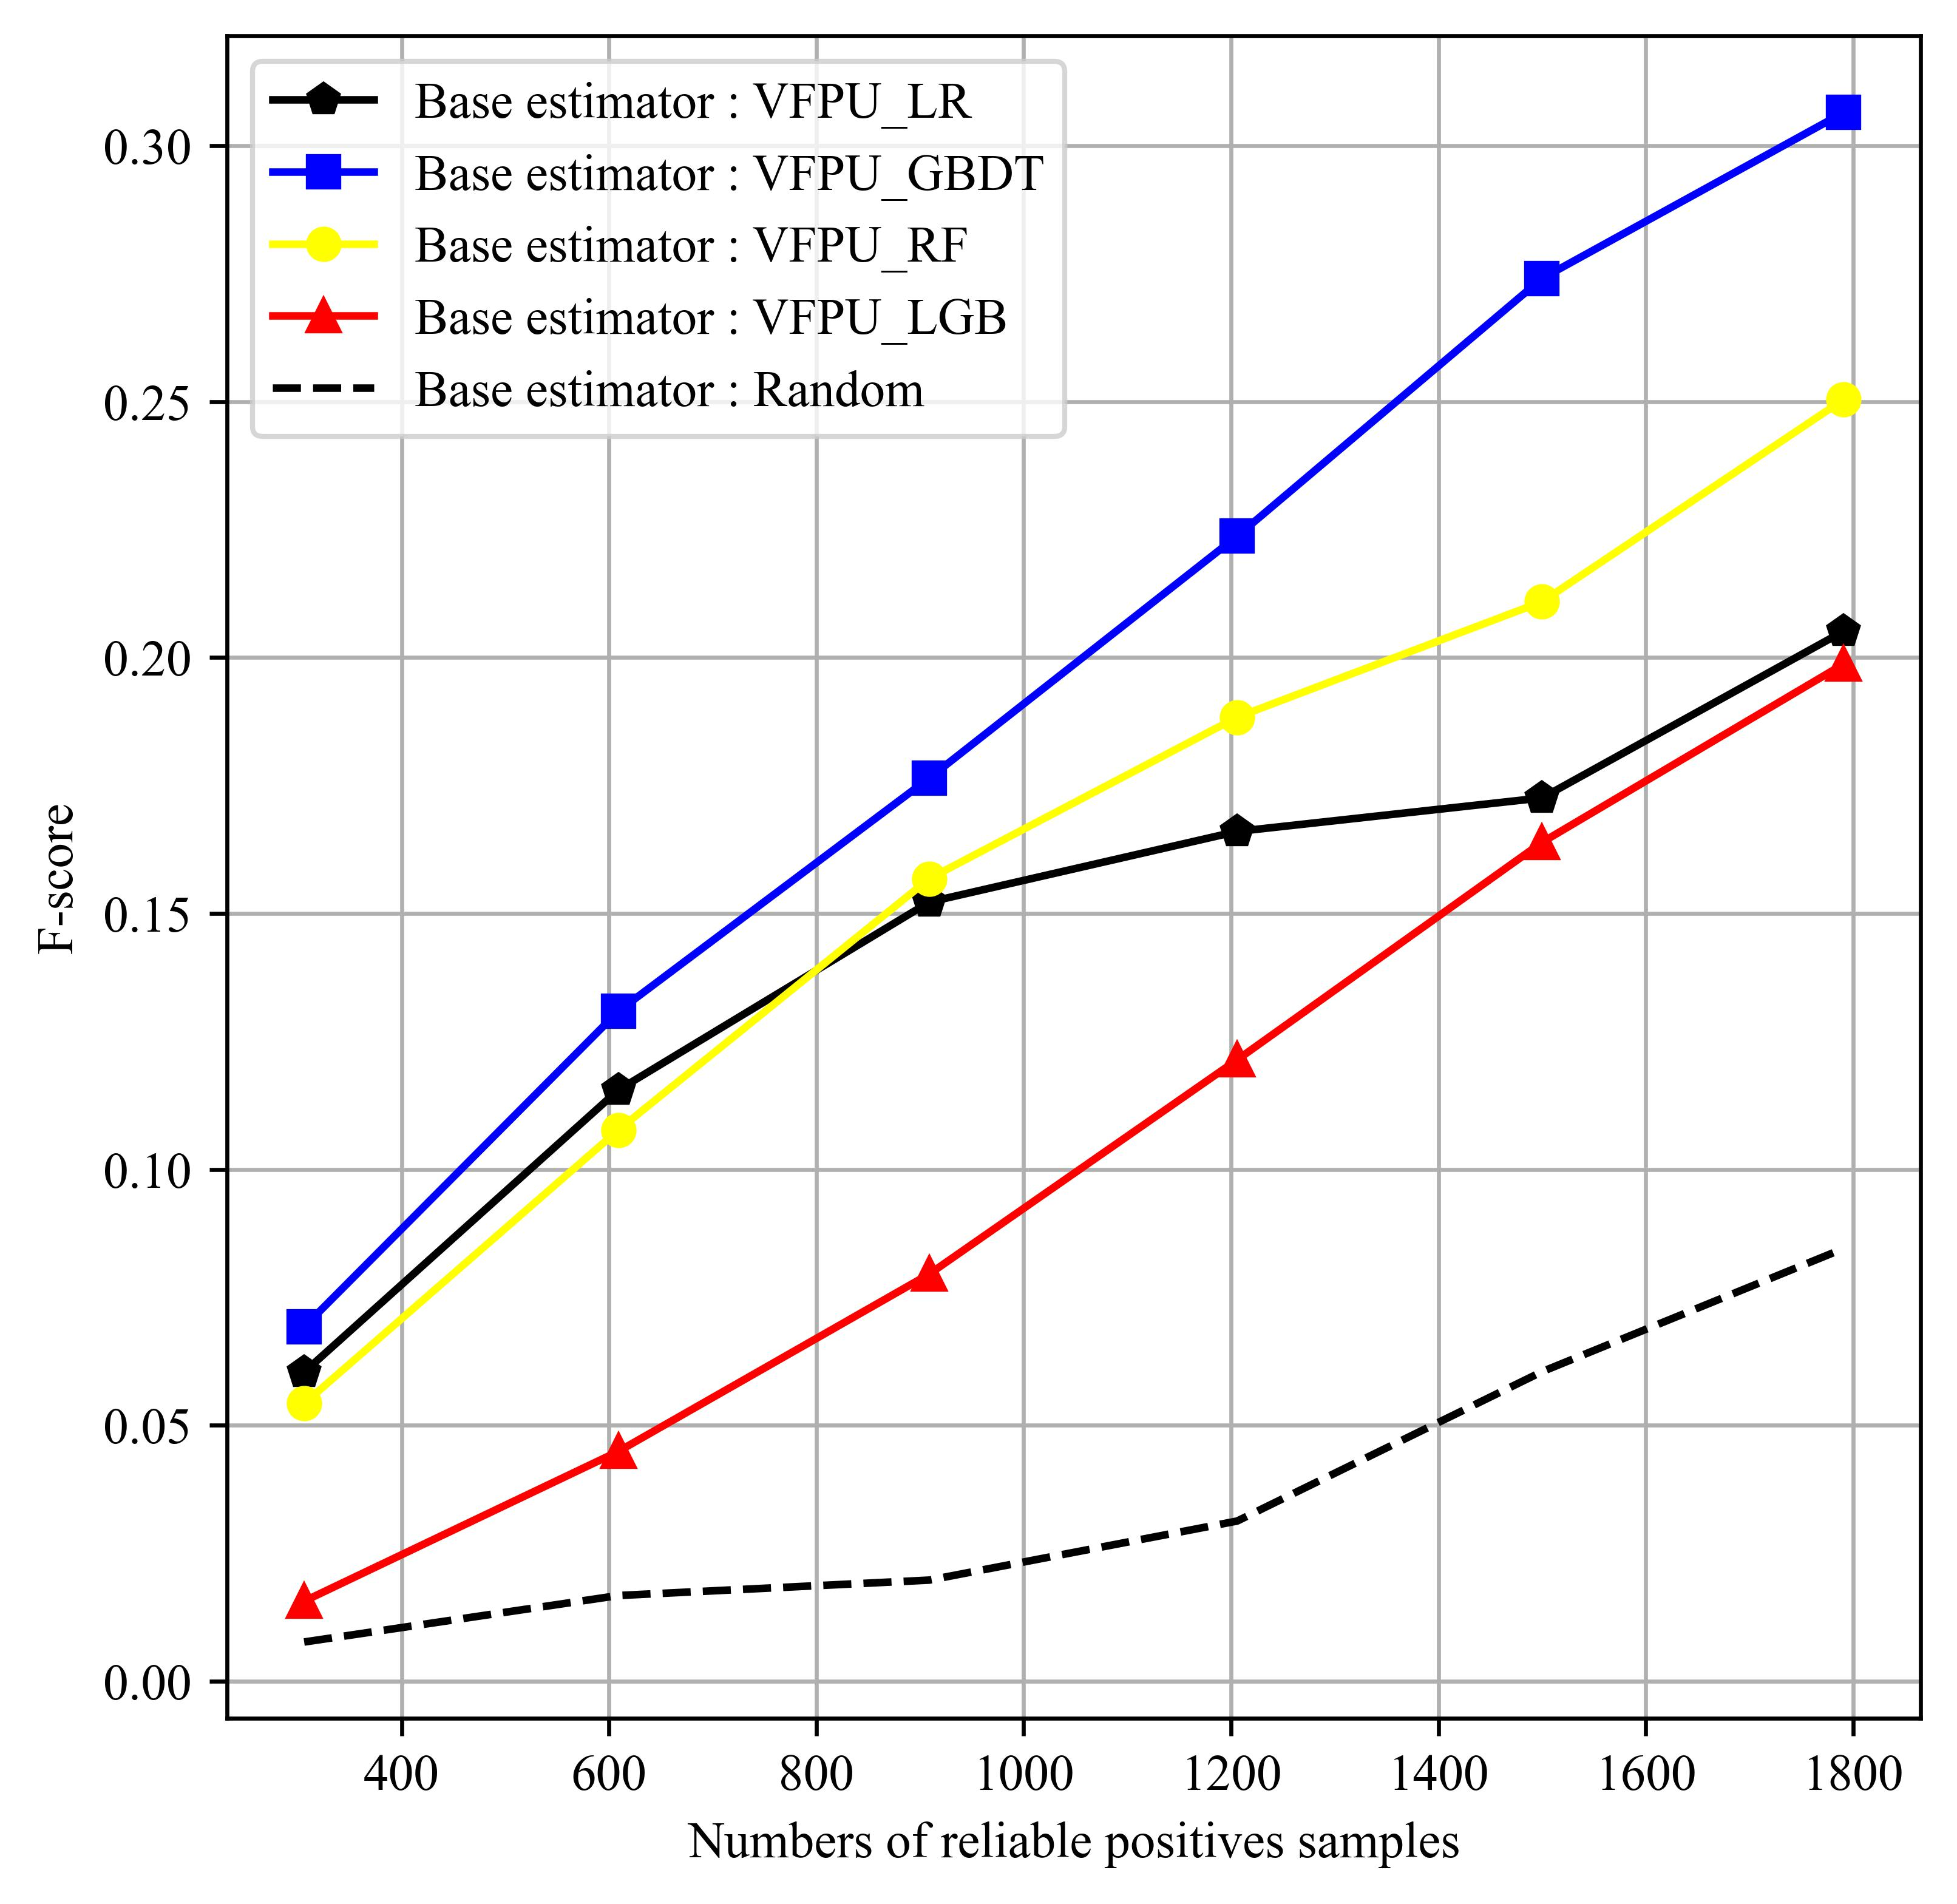
\includegraphics[width=0.45\textwidth,height=4.1cm]{chapters/imgs/Figure 4 (3) in JEPG format}}
	\subfigure[]{\label{RQ2.3.sub4}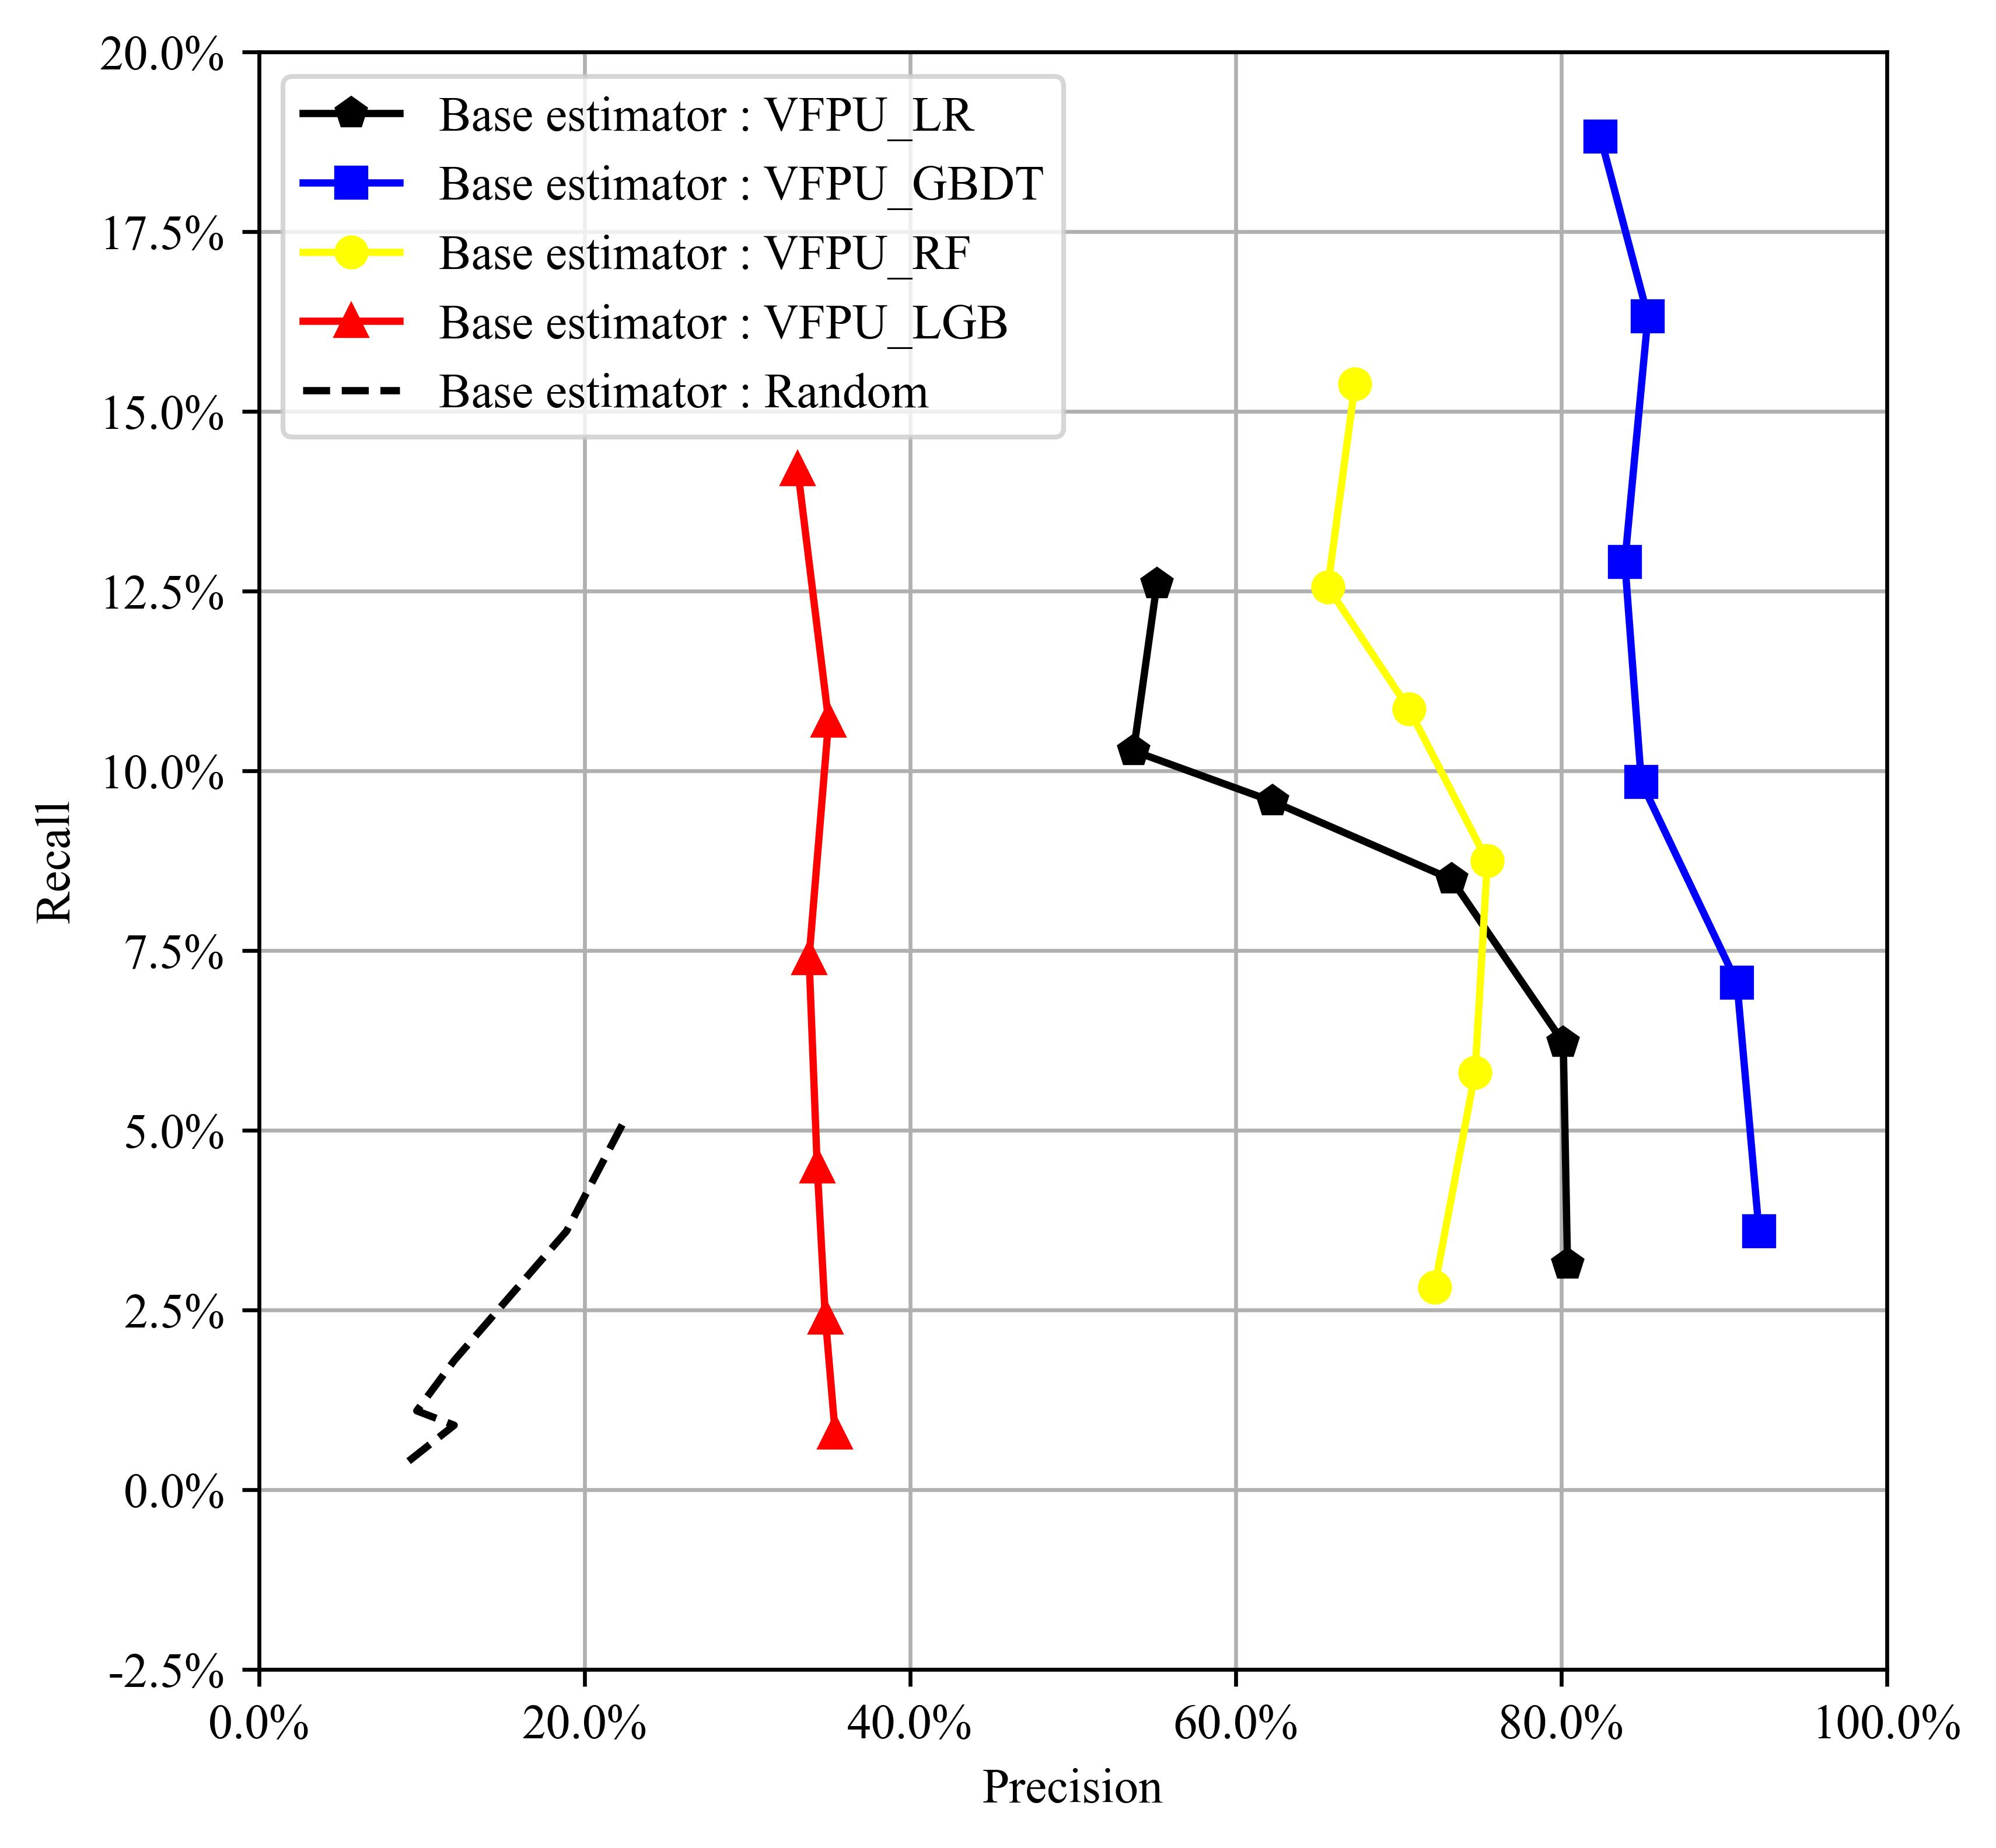
\includegraphics[width=0.45\textwidth,height=4.1cm]{chapters/imgs/Figure 4 (4) in JEPG format}}
	\bicaption[\xiaosi 不同基学器在不同可靠正样本数量下的性能]
	{\centering \songti \wuhao 不同基学器的性能:(a)精度;(b)召回率;(c)F-score;(d)精度-召回率(Census)}
	{\centering \wuhao Base estimators performance: (a) Precision; (b) Recall; (c) F-score; (d) Precision-Recall}
	\label{RQ2.3}
\end{figure}
\vspace{-0.35cm}

此外,图 \ref{RQ2.1.sub4} 中的精确度-召回率曲线进一步验证了VFPU\_GBDT的鲁棒性。通过在各种阈值设置下绘制精确度对召回率的曲线,该曲线有效地捕捉了基学习器的性能动态,特别是在类不平衡是关键问题的场景中。VFPU\_GBDT曲线更接近图的右上象限,表明其在多个阈值下的强大性能——这是不平衡分类任务中高性能模型的标志。

图 \ref{RQ2.2}和 图 \ref{RQ2.3} 提供了VFPU\_GBDT学习器有效性的进一步支持证据。这些图报告了在信用卡违约和成人普查数据集上进行的类似实验。尽管数据集在内在特性和分布属性上有所不同,但这些情况下的实验结果反映了与图 \ref{RQ2.1} 中观察到的相似趋势。VFPU\_GBDT在不同数据集上的一致优越性增强了其在VFPU框架中作为基学习器时的可靠性和有效性。

总结来说,三个基准数据集上的实验结果一致表明,VFPU\_GBDT优于VFPU\_LR、VFPU\_RF、VFPU\_LGB以及基线随机抽样技术。VFPU\_GBDT的优越性能,表现为更高的精确度、召回率和平衡的F-score,使其成为在解决UDD-PU问题时VFPU算法最可靠和推荐的基学习器。因此,在所有后续实验中,采用GBDT作为VFPU方法的基学习器,利用其在挑战性条件下实现准确和平衡分类的明显优势。

\vspace{-0.1cm}
\begin{table}[h]
	\centering
	\renewcommand{\arraystretch}{1.2}
	\bicaption[\xiaosi 不同半监督方法的准确推荐百分比(无联邦)]{\wuhao 不同半监督方法的准确推荐百分比(无联邦)}{\wuhao Accurate recommendations  of semi-supervised methods (non-federated)}
	\label{RQ3.1}
	\resizebox{\textwidth}{!}{
		%		{\songti \wuhao
			\begin{tblr}{
					cells = {c},
					cell{1}{1} = {c=2}{},
					cell{2}{1} = {r=10}{},
					cell{12}{1} = {r=10}{},
					cell{22}{1} = {r=10}{},
					hline{1,32} = {-}{1.5pt},    % Top and bottom lines 1.5pt thick
					hline{2,12,22} = {-}{0.75pt} % Middle lines 0.75pt thick
				}
				\diagbox{Datasets \& Methods}{$num$} &                     & 100              & 700              & 1300             & 1900             & 2100             & 2400             \\
				Bank               & MixMatch            & 32.81\%          & 31.25\%          & 24.85\%          & 20.31\%          & 13.44\%          & 12.03\%          \\
				& FixMatch            & 27.81\%          & 25.47\%          & 24.07\%          & 13.28\%          & 12.66\%          & 12.50\%          \\
				& CoMatch             & 31.56\%          & 24.85\%          & 24.07\%          & 17.19\%          & 12.50\%          & 12.03\%          \\
				& AdaMatch            & 33.56\%          & 30.50\%          & 25.78\%          & 20.63\%          & 18.13\%          & 17.19\%          \\
				& SoftMatch           & 32.81\%          & 31.56\%          & 24.53\%          & 19.38\%          & 17.19\%          & 12.50\%          \\
				& \_GBDT              & 53.65\%          & 47.00\%          & 33.62\%          & 28.99\%          & 29.17\%          & 29.33\%          \\
				& Bagging\_GBDT       & 42.74\%          & 33.46\%          & 28.22\%          & 31.67\%          & 27.03\%          & 26.00\%          \\
				& 2Step\_GBDT         & 49.79\%          & 42.79\%          & 29.72\%          & 33.38\%          & 31.30\%          & 26.85\%          \\
				& Pseudo-Labelling    & 33.30\%          & 22.00\%          & 21.80\%          & 24.10\%          & 23.00\%          & 22.70\%          \\
				& No\_Fed\_VFPU\_GBDT & \textbf{77.00\%} & \textbf{66.86\%} & \textbf{59.62\%} & \textbf{54.26\%} & \textbf{53.95\%} & \textbf{52.38\%} \\
				Credit             & MixMatch            & 29.29\%          & 25.34\%          & 24.09\%          & 23.88\%          & 23.47\%          & 21.18\%          \\
				& FixMatch            & 27.00\%          & 25.34\%          & 23.88\%          & 22.85\%          & 22.43\%          & 21.39\%          \\
				& CoMatch             & 26.79\%          & 25.55\%          & 24.09\%          & 23.47\%          & 22.85\%          & 21.18\%          \\
				& AdaMatch            & 26.79\%          & 25.34\%          & 25.13\%          & 22.85\%          & 22.63\%          & 21.18\%          \\
				& SoftMatch           & 26.38\%          & 24.09\%          & 23.47\%          & 22.43\%          & 21.18\%          & 20.97\%          \\
				& \_GBDT              & 42.80\%          & 34.62\%          & 31.56\%          & 29.89\%          & 28.65\%          & 25.43\%          \\
				& Bagging\_GBDT       & 42.74\%          & 30.40\%          & 25.52\%          & 26.17\%          & 26.91\%          & 24.55\%          \\
				& 2Step\_GBDT         & 42.74\%          & 33.29\%          & 31.77\%          & 26.24\%          & 27.57\%          & 26.00\%          \\
				& Pseudo-Labelling    & 38.40\%          & 32.50\%          & 30.90\%          & 29.20\%          & 28.40\%          & 27.30\%          \\
				& No\_Fed\_VFPU\_GBDT & \textbf{51.25\%} & \textbf{50.14\%} & \textbf{47.69\%} & \textbf{41.82\%} & \textbf{40.82\%} & \textbf{39.82\%} \\
				Census             & MixMatch            & 37.72\%          & 36.39\%          & 36.05\%          & 34.15\%          & 32.81\%          & 32.59\%          \\
				& FixMatch            & 38.84\%          & 37.28\%          & 36.39\%          & 34.38\%          & 33.93\%          & 32.36\%          \\
				& CoMatch             & 37.18\%          & 34.06\%          & 32.97\%          & 31.38\%          & 31.38\%          & 31.38\%          \\
				& AdaMatch            & 38.39\%          & 37.50\%          & 36.24\%          & 35.49\%          & 34.38\%          & 33.93\%          \\
				& SoftMatch           & 38.84\%          & 35.94\%          & 35.04\%          & 33.93\%          & 32.81\%          & 29.91\%          \\
				& \_GBDT              & 64.00\%          & 61.00\%          & 58.00\%          & 54.00\%          & 51.00\%          & 54.00\%          \\
				& Bagging\_GBDT       & 68.00\%          & 59.00\%          & 54.00\%          & 52.00\%          & 48.00\%          & 51.00\%          \\
				& 2Step\_GBDT         & 66.00\%          & 63.00\%          & 56.00\%          & 51.00\%          & 52.00\%          & 53.00\%          \\
				& Pseudo-Labelling    & 42.90\%          & 29.30\%          & 28.40\%          & 41.40\%          & 37.30\%          & 45.30\%          \\
				& No\_Fed\_VFPU\_GBDT & \textbf{99.00\%} & \textbf{99.43\%} & \textbf{94.57\%} & \textbf{84.08\%} & \textbf{80.08\%} & \textbf{75.08\%} 
			\end{tblr}
			%		}	
	}
\end{table}
\vspace{-0.5cm}

实验三:基线对比实验,表 \ref{RQ3.1} 显示,提出的No\_Fed\_VFPU\_GBDT方法在所有测试数据集上以及对于各个不同的$num$值均持续优于其他九种半监督方法。例如,在Census数据集中,当$num=1300$时,VFPU\_GBDT实现了最高的推荐准确率94.57\%。这一显著性能与基线方法形成了鲜明对比:\_GBDT、2Step\_GBDT和Bagging\_GBDT分别仅达到54\%、56\%和54\%的准确率。同时,基于深度学习的方法——MixMatch、FixMatch、CoMatch、AdaMatch和SoftMatch——的推荐准确率明显较低,分别为36.05\%、36.39\%、32.97\%、36.24\%和35.04\%。

尽管Match系列算法代表了半监督学习领域的最新进展,其表现不佳可以归因于两个关键因素。首先,这些方法本质上需要大量标记数据,涵盖正类和负类。然而,在PU问题情境下,负样本并未被明确标记,这使得这些算法处于明显的不利地位。其次,使用Wide ResNet-28模型这一相对复杂的深度学习网络,在面对类分布极度不平衡的数据集时,可能无意中导致过拟合。这种过拟合会削弱模型的泛化能力,从而导致整体性能较低。

\vspace{-0.1cm}
\begin{table}[h]
	\centering
	\bicaption[\xiaosi 不同半监督方法的准确推荐百分比(纵向联邦)]
	{\wuhao 不同半监督方法的准确推荐百分比(纵向联邦)}
	{\wuhao Accurate recommendations  of semi-supervised methods (in VFL)}
	\label{RQ3.2}
	\resizebox{\textwidth}{!}{
		% 整体使用 {\songti \wuhao ...} 包裹表格内容
		{\songti \wuhao
			\begin{tblr}{
					column{1} = {c},
					column{2} = {c},
					cell{1}{1} = {c=2}{},
					cell{2}{1} = {r=4}{},
					cell{6}{1} = {r=4}{},
					cell{10}{1} = {r=4}{},
					hline{1} = {-}{1.5pt}, % 顶部粗线
					hline{2} = {-}{}, % 表头下方普通线
					hline{6,10} = {-}{}, % 数据区域中的普通横线
					hline{14} = {-}{1.5pt}, % 底部粗线
				}
				\diagbox{Datasets \& Methods}{$num$} &                  & 100              & 700              & 1300             & 1900             & 2100             & 2400             & runtime(s)        \\
				Bank               & VF\_GBDT         & 7.00\%           & 5.30\%           & 4.70\%           & 5.10\%           & 5.00\%           & 4.80\%           & 10673.81          \\
				& VF\_Bagging GBDT & 17.00\%          & 18.90\%          & 19.70\%          & 20.30\%          & 20.70\%          & 20.80\%          & 15069.88          \\
				& VF\_2Step GBDT   & 4.00\%           & 3.60\%           & 5.30\%           & 5.40\%           & 6.50\%           & 7.40\%           & 44030.4           \\
				& VFPU\_GBDT       & \textbf{74.00\%} & \textbf{63.10\%} & \textbf{59.00\%} & \textbf{54.20\%} & \textbf{53.20\%} & \textbf{52.30\%} & \textbf{106922.2} \\
				Credit             & VF\_GBDT         & 18.00\%          & 22.60\%          & 22.10\%          & 21.40\%          & 21.60\%          & 22.30\%          & 12025.47          \\
				& VF Bagging GBDT  & 32.00\%          & 23.90\%          & 23.50\%          & 23.30\%          & 22.30\%          & 22.00\%          & 15791.59          \\
				& VF\_2Step GBDT   & 24.00\%          & 25.40\%          & 23.70\%          & 22.30\%          & 22.30\%          & 22.00\%          & 46954.19          \\
				& VFPU\_GBDT       & \textbf{44.00\%} & \textbf{48.86\%} & \textbf{44.85\%} & \textbf{39.47\%} & \textbf{38.33\%} & \textbf{37.43\%} & \textbf{107075.9} \\
				Census             & VF\_GBDT         & 19.00\%          & 25.40\%          & 23.90\%          & 23.10\%          & 22.90\%          & 22.80\%          & 11581.47          \\
				& VF\_Bagging GBDT & 13.00\%          & 19.90\%          & 22.30\%          & 23.20\%          & 23.20\%          & 23.90\%          & 15987.59          \\
				& VF\_2Step GBDT   & 25.00\%          & 23.10\%          & 24.30\%          & 24.60\%          & 25.00\%          & 25.60\%          & 46808.19          \\
				& VFPU\_GBDT       & \textbf{98.00\%} & \textbf{98.71\%} & \textbf{94.23\%} & \textbf{80.53\%} & \textbf{76.05\%} & \textbf{72.74\%} & \textbf{107089.9} 
			\end{tblr}
		}
	}
\end{table}
\vspace{-0.3cm}

相比之下,PU学习方法,包括VFPU\_GBDT、\_GBDT、Bagging\_GBDT和2Step\_GBDT,专门为解决在主要由未标记样本构成的数据集中揭示隐藏正样本这一挑战而设计。这些方法利用数据的内在结构,并采用定制的策略来迭代细化对潜在正实例的识别。因此,如表 \ref{RQ3.1}所示,表现最好的四种方法分别为\_GBDT、Bagging\_GBDT、2Step\_GBDT和VFPU\_GBDT。它们的出色性能凸显了PU学习策略在负样本不可直接获得且数据存在显著不平衡的情景中的有效性。

通过对打分机制、超参数设置以及底层模型架构的详细讨论,丰富了分析内容,从而全面理解了实验设置及各方法的相对优劣。这一详细论述凸显了提出的No\_Fed\_VFPU\_GBDT方法在有效揭示隐藏正样本方面的优势,为未来在常规PU学习和联邦PU学习框架下的研究提供了宝贵的启示。

在第二个实验中,将第一个实验中表现最佳的四种方法适配到纵向联邦学习(VFL)环境中,分别标记为VF\_GBDT、VF\_Bagging\_GBDT、VF\_2Step\_GBDT和VFPU\_GBDT。此外,为了评估这些方法在VFL环境中部署时的时间复杂度和计算开销,在$num = 2400$的各种数据集上仔细记录了每种方法的训练时间。训练时间表示为runtime(s),其中s代表秒,详细内容见表 \ref{RQ3.2}。

表 \ref{RQ3.2} 与表 \ref{RQ3.1} 类似,展示了VFL设置下不同方法所达到的准确率百分比的比较分析。结果清晰地表明,VFPU\_GBDT方法在推荐准确率方面始终优于其他三种方法。例如,在Census数据集上,当$num=1000$时,VFPU\_GBDT达到了显著高的98.70\%的推荐准确率,这明显高于VF\_GBDT、VF\_Bagging\_GBDT和VF\_2Step\_GBDT的准确率,它们分别为24.20\%、21.10\%和24.30\%。在Credit数据集上,尽管VFPU\_GBDT展示了更高的准确率,但它带来了更高的计算成本:本章的方法记录的运行时间为107075.9s,而VF\_GBDT、VF\_Bagging\_GBDT和VF\_2Step\_GBDT的运行时间分别为12025.47s、15791.59s和46954.19s。

\vspace{-0.1cm}
\begin{figure}[h]
	\centering 
	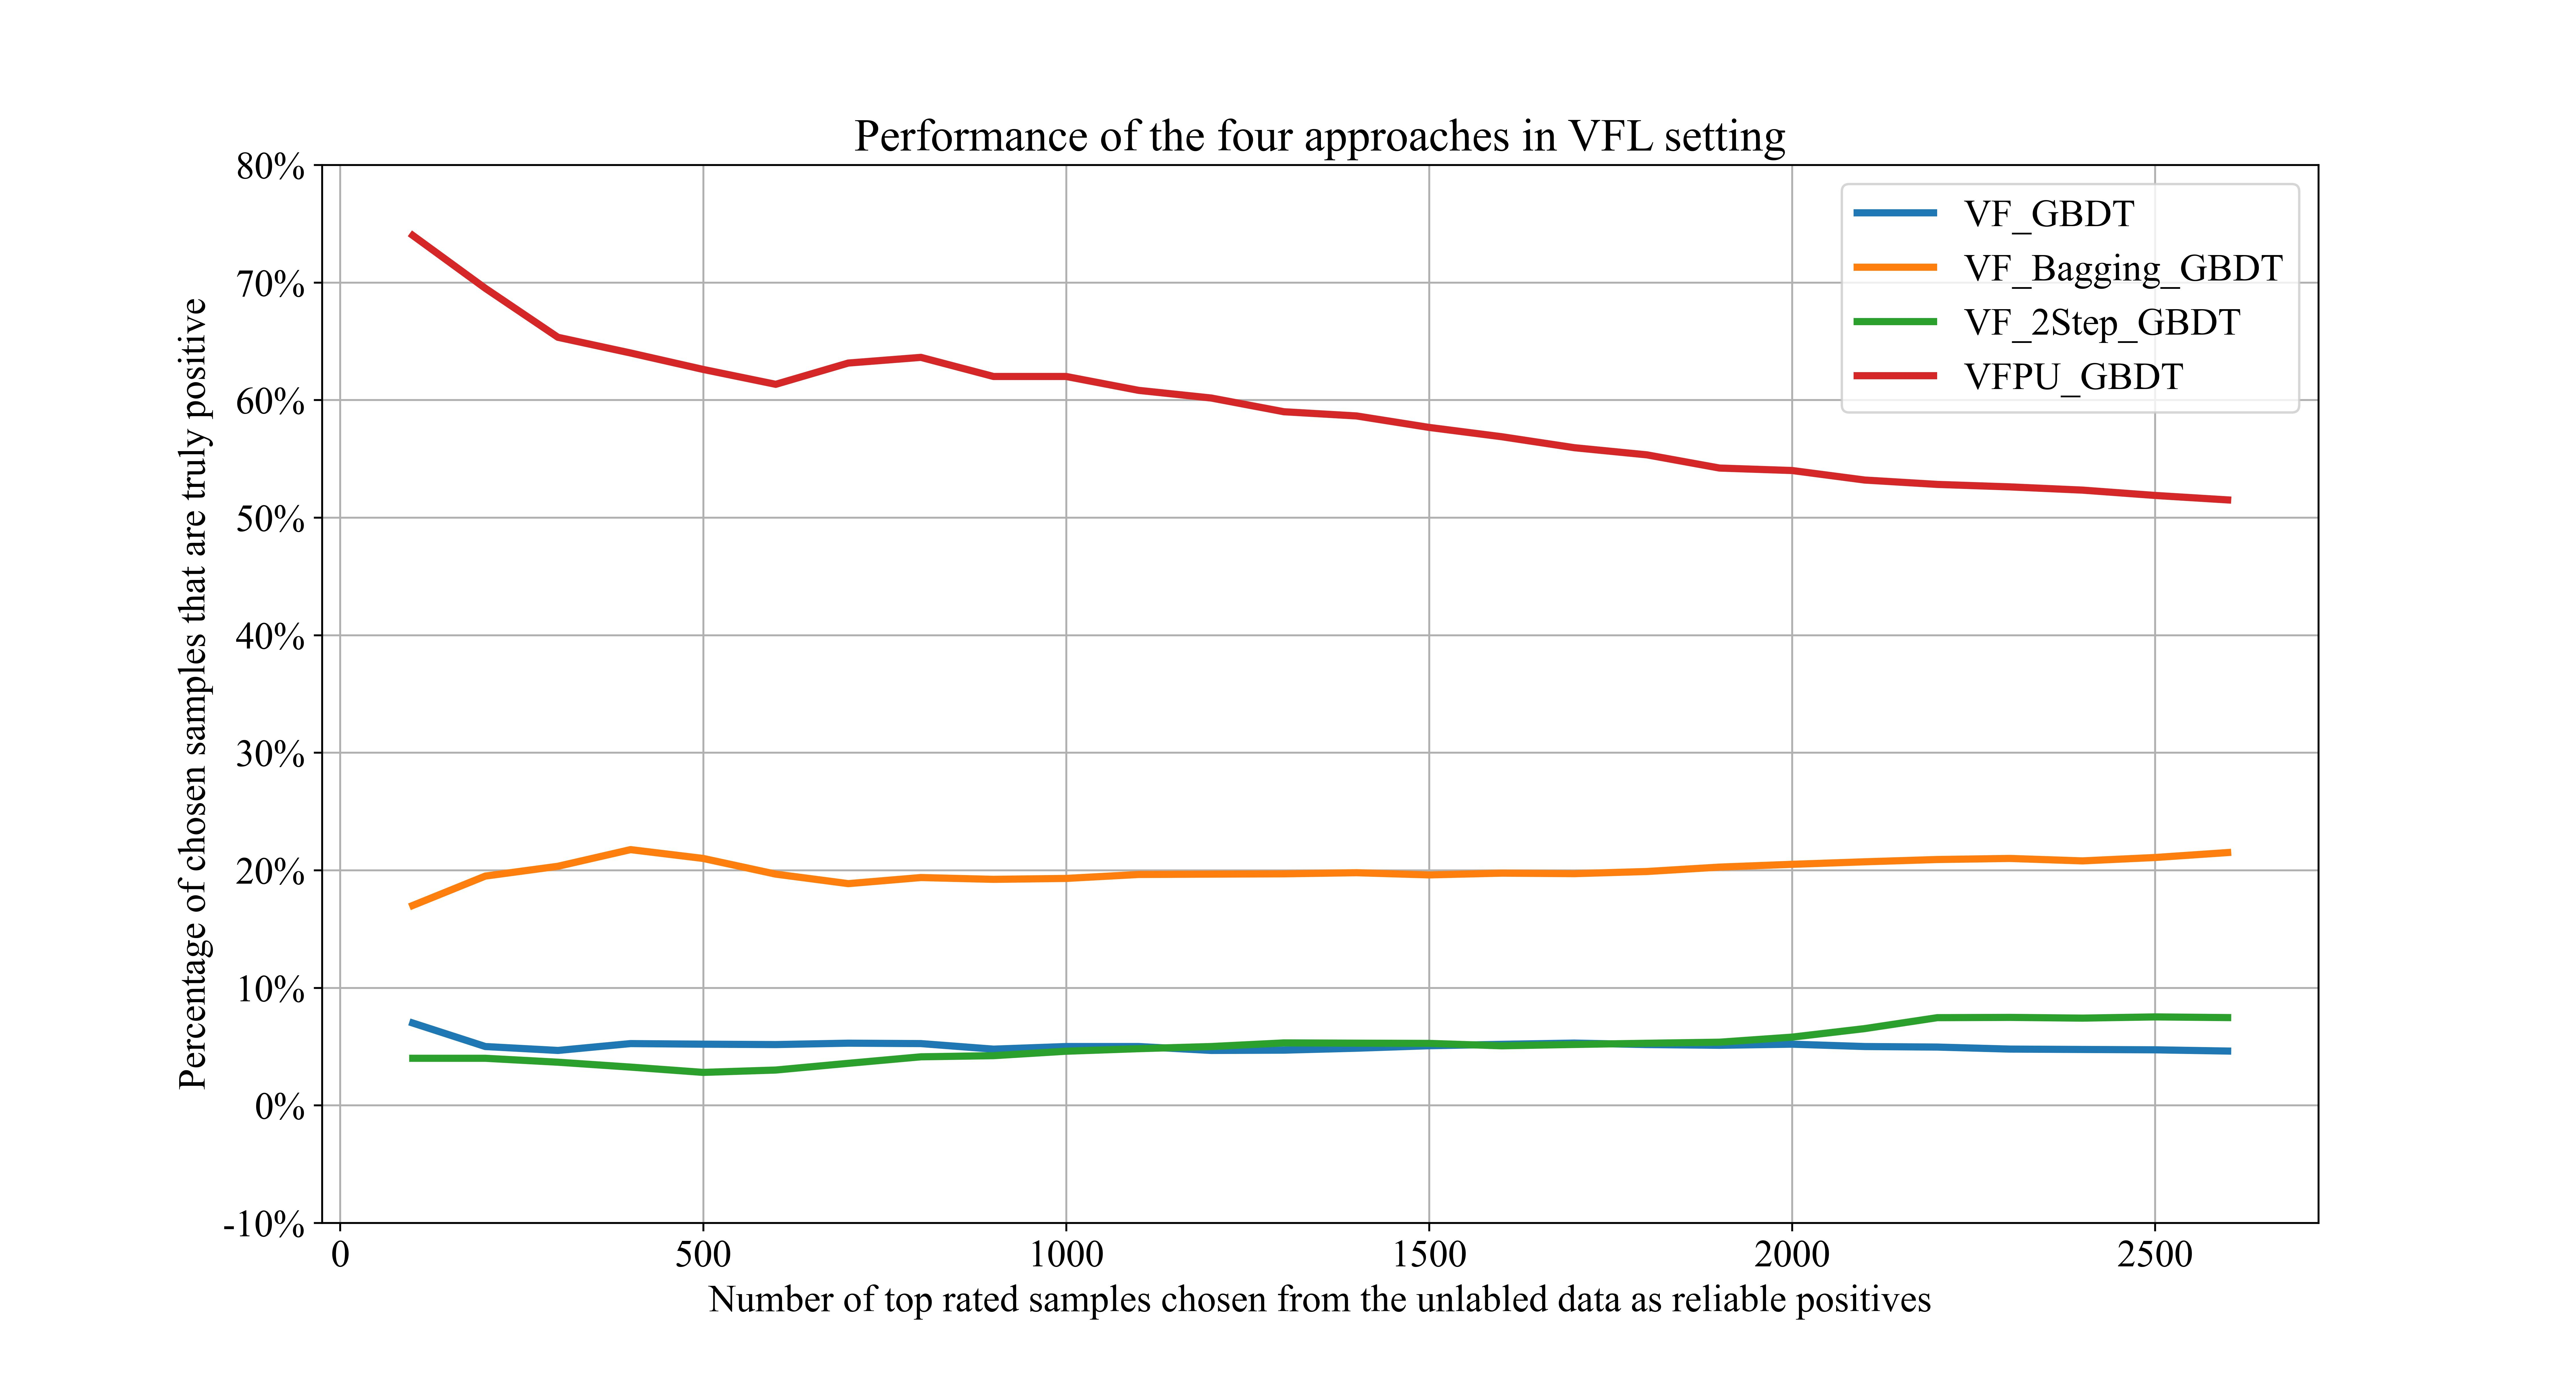
\includegraphics[width=0.9\textwidth]{chapters/imgs/Figure 5 in JPEG format}
	\bicaption[\xiaosi 不同半监督方法在纵向联邦学习(VFL)中的准确推荐百分比]
	{\centering \wuhao 不同半监督方法在纵向联邦学习(VFL)中的准确推荐百分比(Bank 数据集)}
	{\centering \wuhao The accurate recommendations percentage by Different Semi-supervised Methods in VFL (The Bank Marketing Dataset)}
	\label{fig:GBDT}
\end{figure}
\vspace{-0.35cm}

值得注意的是,按runtime(s)指标衡量,VFPU\_GBDT的耗时约为其他方法的10倍。这种增加的时间消耗主要是由于VFPU\_GBDT在选择可靠正样本时采用了更为谨慎和迭代的策略。该算法采用多次迭代,每次迭代只选择一小部分样本,确保只有最可靠和准确预测的正样本被选中。这种谨慎的选择过程引入了额外的计算开销。然而,这种训练时间与推荐准确率之间的权衡被认为是可接受的,因为准确率的显著提高证明了额外训练时间的合理性。

图  \ref{fig:GBDT} 提供了表 \ref{RQ3.2} 中讨论的银行营销数据集实验结果的可视化表示。在该图中,x轴表示被选为可靠正样本的评分最高的未标记样本数量,而y轴表示这些被选择样本中真正为正样本的百分比。图中清晰地说明,随着$num$从100增加到1000,VFPU\_GBDT识别的隐藏正样本数量迅速减少。这种观察到的减少可归因于几个因素。最初,与正类表现出强烈相似性或与负类有明显差异的未标记数据样本被迅速识别和选择。然而,随着选择过程的继续,剩余的未标记数据往往在正负类之间表现出特征重叠,这给基学习器带来干扰。这种干扰导致错误分类,从而降低了准确推荐的百分比。虽然其他方法在不同$num$值下表现相对稳定,但这种表面上的稳定性并不一定是有利的。这些方法始终较低的准确推荐百分比表明它们在可靠识别隐藏正样本方面能力有限。此外,考虑到未标记数据集中只有约2500个真正的正样本,当选择的正样本数量超过这个阈值时,VFPU\_GBDT的准确率自然会下降。

总之,实验结果提供了强有力的证据,表明VFPU\_GBDT算法在VFL环境中推荐可靠正样本方面非常有效。尽管需要额外的计算时间,但推荐准确率的显著提升使VFPU\_GBDT相比其他半监督方法成为更优方案。这项实验凸显了在联邦学习环境中应用VFPU\_GBDT算法解决未标记数据缺乏的PU(UDD-PU)学习推荐问题的显著优势,强调了它在高准确率至关重要的实际应用中的潜力。

\section{本章小结}
本章主要介绍了未标记数据缺乏的PU(UDD-PU)学习问题,其中需要模型训练的一方仅持有正样本数据,而其他参与方拥有大量未标记数据。为解决UDD-PU问题,本章提出了一种基于半监督学习的多方联邦推荐方法。具体而言,设计了VFPU算法作为该方法的核心,该算法有效整合了两种PU学习技术,并将其适配到纵向联邦学习框架中。通过这种方式,VFPU能够利用有限的标记数据(正样本)和丰富的未标记数据来提高推荐模型的性能。在三个数据集上评估了所提出的方法,并将其与其他半监督学习方法进行了比较。实验结果明确表明,VFPU算法在确保数据隐私的同时,与非联邦方法相比只有很小的性能下降,就能达到令人满意的性能。此外,证明了VFPU算法在纵向联邦学习环境中发现隐藏正样本方面始终优于其他半监督学习方法。而且,对不同基学习器的分析表明,梯度提升决策树(VFPU\_GBDT)在精确率、召回率和F值方面持续展现出卓越的性能。这一发现强调了为VFPU算法选择适当基学习器的重要性,以便在各种实际应用中优化其性能。